\documentclass[a4paper]{article}
% !Rnw weave = Sweave

\title{DICE User Manual}
\author{Predictive Science Inc.}

%\usepackage[round]{natbib}
\usepackage{cite} 		% enhance multi-citation aesthetics
\usepackage{graphicx, Rd}
\usepackage{listings}
\usepackage{amsmath}

% Loosen float-placement requirements
    \renewcommand{\topfraction}{0.9}	% max fraction of floats at top
    \renewcommand{\bottomfraction}{0.8}	% max fraction of floats at bottom
    %   Parameters for TEXT pages (not float pages):
    \setcounter{topnumber}{2}
    \setcounter{bottomnumber}{2}
    \setcounter{totalnumber}{4}     % 2 may work better
    \setcounter{dbltopnumber}{2}    % for 2-column pages
    \renewcommand{\dbltopfraction}{0.9}	% fit big float above 2-col. text
    \renewcommand{\textfraction}{0.07}	% allow minimal text w. figs
    %   Parameters for FLOAT pages (not text pages):
    \renewcommand{\floatpagefraction}{0.70}	% require fuller float pages

\lstset{frame=trbl,basicstyle=\small\tt}
\usepackage{hyperref}
\usepackage{color}
\definecolor{Blue}{rgb}{0,0,0.8}
\hypersetup{%
colorlinks,%
plainpages=true,%
linkcolor=black,%
citecolor=black,%
urlcolor=Blue,%
%pdfstartview=FitH,% or Fit
pdfstartview={XYZ null null 1},%
pdfview={XYZ null null null},%
pdfpagemode=UseNone,% for no outline
pdfauthor={Friedrich Leisch and R-core},%
pdftitle={DICE user Manual},%
pdfsubject={R vignette documentation system}%
}

\sloppy

\usepackage{Sweave}

\begin{document}
\Sconcordance{concordance:dice.tex:dice.Rnw:%
1 866 1 1 12 45 0 1 2 405 1}

\maketitle

\setcounter{tocdepth}{2}
\tableofcontents

%\SweaveOpts{engine=R, keep.source=TRUE}
%\SweaveOpts{eps=FALSE, pdf=TRUE, width=8, height=5.5, strip.white=true}
\section{Introduction}
\label{sec:intro}

The \pkg{DICE} package implements a global model of both directly transmitted and vector-borne diseases within populations with arbitrary spatial resolution, with the objective of making best use of available data at different spatial scales.  Building on previous work which was limited to influenza and a single spatial region \cite{riley13a, riley15a}, \pkg{DICE} uses either mechanistic compartmental models or statistical techniques to fit and when relevant forecast the time evolution of the disease.   The deterministic compartmental models (SIR, SEIR etc.), are applied on various interacting spatial scales, and use a robust Markov-Chain-Monte-Carlo (MCMC) fitting procedure that can quickly characterize disease incidence profiles, of either coupled or uncoupled regions, in real-time providing estimates for:
\begin{itemize}
\item Within, and if applicable between, region epidemic transmissibility (measured by the basic reproduction number $R_e$ and the next-generation matrix \cite{mills2014spatial}, if applicable)
\item individual level epidemic severity (as described by the proportion $p_C$ of infections that result in clinical cases)
\end{itemize}
The statistical techniques are based on Seasonal Autoregressive Integrated Moving Average (SARIMA) models which have received the most attention in this field.
\pkg{DICE} uses a MySQL database which includes incidence profiles for a large number of directly transmitted and vector-borne diseases along with population and climate data (precipitation, temperature and specific humidity). These data sets are provided on spatial scales of various, increasing, resolutions. For each data source/disease, the incidence, population and climate data use the same spatial and temporal scales. The latter can be either daily, weekly, monthly or yearly. School opening/closing schedules for the US are also included in the database. This dataset, along with the specific humidity data, are needed for three of the four different models for the time dependence of the basic reproduction number $R_{e}(t)$ that the user can choose from. The school and climate data can also be used as covariates when fitting/forecasting the incidence using the SARIMA statistical methods. \pkg{DICE} also includes a compact data set of Military Data for the 2009-2010 H1N1 pandemic season.  This Military data set includes weekly numbers of ILI cases along with school vacation schedule and specific humidity for $50$ military bases. The \pkg{DICE} MySQL database can be explored using a series of web based tools described here \url{http://predsci.com/id_data/}.


Upon completion of the MCMC fitting or statistical procedure, the \pkg{DICE} package analyzes the results and produces an extensive set of publication-quality plots (in a  PDF or PNG format) and tables (in .csv format).
The complete history of the run and the fitting procedure is saved as an \file{RData} file which the user can later load and further analyze.


\section{Quick Start Guide}
The \pkg{DICE} package is accessible as a GitHub repository.  Before downloading the repository, there are a few software requirements:


\subsection{Installation Instructions}
\label{sssec:Install}
In a command line environment navigate to the directory `mydir' where you would like the source code for \pkg{DICE} to be located
\begin{verbatim}
cd /.../mydir
\end{verbatim}
and clone from GitHub
\begin{verbatim}
git clone https://github.com/predsci/DICE.git
\end{verbatim}
This creates a sub-directory ``DICE" that contains all of the files required to compile.  For a global install, execute the provided python compile script:
\begin{verbatim}
cd DICE
./compile.py
\end{verbatim}
For a local install, execute the following commands:
\begin{verbatim}
cd DICE
/bin/rm -rf DICE_1.0.tar.gz dice/src/*.o dice/src/*.so
R CMD build DICE
R CMD INSTALL -l /.../mylib DICE
\end{verbatim}
where `mylib' is the local directory in which you would like to store the R library.  A common problem encountered here is that for Mac OS X, the fortran libraries \code{-lgfortran}, \code{-lquadmath}, and \code{-lm} are not located where R expects them.  This will result in an error like:
\begin{verbatim}
ld: library not found for -lgfortran
\end{verbatim}
following a call to \code{clang}.  This can be corrected by opening ``/Library/Frameworks/R.framework/Resources/etc/Makeconf" and changing the ``FLIBS" variable to point at the location of libgfortran.a and libquadmath.a in the user's local installation.  In one case this meant changing
\begin{verbatim}
FLIBS = -L/usr/local/lib/gcc/x86_64-apple-darwin13.0.0/4.8.2 -lgfortran
    -lquadmath -lm
\end{verbatim}
to
\begin{verbatim}
FLIBS = -L/opt/local/lib/gcc5/gcc/x86_64-apple-darwin15/5.3.0 -lgfortran
    -lquadmath -lm
\end{verbatim}
for R to find the fortran libraries installed with gcc5.3 via MacPorts.  When unsure about the correct directory, it is suggested to search your file system for `libgfortran.a' and try the corresponding directory.  Similarly, the ``F77" variable in Makeconf dictates which fortran compiler is called.  Depending on the version of R, this defaults to ``F77 = gfortran-A.B".  In the case mentioned above (gcc compiler installed via MacPorts), changing
\begin{verbatim}
F77 = gfortran-4.8
\end{verbatim}
to
\begin{verbatim}
F77 = gfortran
\end{verbatim}
allowed R to call the fortran compiler correctly.

To check that the package installed, open an R environment and enter
\begin{verbatim}
require("DICE")
\end{verbatim}
This will load the \pkg{DICE} package as well as a number of dependency packages.  No errors on load generally indicates a successful compile.  The following section presents some example scripts to begin running \pkg{DICE}.

\subsection{Examples}
\label{sec:exmpl}
In this section we define the minimal, most important, set of  parameters that the user will need to set for a \pkg{DICE} run. We focus on the parameters that control the main features of the package and discuss what values to choose for them for a few useful examples.  For a more detailed description of the parameters the users should consult sections \ref{sec:MechModeling} and \ref{sec:data}.


The \pkg{DICE} package is currently set to run using either a MySQL database or by directly accessing the the CDC influenza-like-illness database for the most up-to-date data.  The user should first choose a disease to study (e.g. dengue, influenza), a country (or region) and season, and a method (mechanistic or statistical). Once these have been selected other choices can be made that are specific to the method used and the disease.  For example, in the case of a mechanistic method (and provided that incidence data is available) the user should choose if to model the country/region directly or as a coupled or uncoupled aggregate of higher resolution sub-regions.  The user can also select a specific compartmental model (e.g. SIR, SEIR and models that describe both the human and the vector states explicitly). Additional selections control the details of the MCMC fitting procedure. We recommend using our web based tools to explore the database.

\subsubsection{Setting Up and Running DICE}

After selecting the $disease$ (e.g. `flu'), country (e.g. `usa'), and  $method$ (`stat' or `mech') the user should choose  a season by setting the parameter $year$ to the start year of the season (e.g. for the 2015-2016 influenza season use: $year=2015$). The spatial region we want to model and at what level of granularity we want to do it are controlled by the parameters mod$\_$level and fit$\_$level, respectively. In the case of CDC data (first example below), data is publicly available on the national, regional (the regions are the ten HHS regions, see figure  \ref{fig:CDCregs}), and state levels.  In the first example below we set $mod\_level = 2$ and $fit\_level = 3$.  This choice means that we are modeling the national incidence data using the ten HHS regional-level incidence data.  We also want the HHS regions to be coupled and therefore set: $isingle=0$.  (With these choices the national level curve we are modeling is a result of both within and between region infections.)
The following command produces a quick exploratory \pkg{DICE} run:

\begin{verbatim}
> output <- runDICE(disease = 'flu', RegState = 'usa', method = 'mech',
            year = 2017, mod_level = 2, fit_level = 3, isingle = 0)
\end{verbatim}


If we want to keep all of our choices the same but decouple the ten HHS regions so that our prediction for the national CDC profile is a weighted sum of our best predictions for each of the ten HHS regions, we only change the parameter $isingle$ from zero to one:


\begin{verbatim}
> output <- runDICE(disease = 'flu', RegState = 'usa', method = 'mech',
            year = 2017, mod_level = 2, fit_level = 3, isingle = 1)
\end{verbatim}
With this choice, infection can only happen within each HHS region and there is no interaction between the regions. As explained in detail in section \ref{sec:MechModeling} this still allows each region to have it's  own set of optimal parameters, e.g. epidemic onset time, force of infection etc..

To demonstrate how to model a single HHS region using its' state level data we use the CDC dataset, $disease = ``flu"$, and set: $mod\_level=3$ and $fit\_level=4$.  We choose the 2014-2015 season, $year=2014$, HHS region number 9 ($RegState = 9$) with coupling between the states that make-up this region ($isingle=0$):
\begin{verbatim}
> output <- runDICE(disease = 'flu', RegState = 9, year = 2014, mod_level = 3,
            fit_level = 4, isingle = 0)
\end{verbatim}

In these two examples the \pkg{DICE} code was using the default SIR compartmental model.  To use an SEIR model for the flu set $epi\_model = ``SEIR"$ or $epi\_model = 2$ :

\begin{verbatim}
> output <- runDICE(disease = 'flu', RegState = 'usa', method = 'mech',
            year = 2017, mod_level = 2, fit_level = 3, isingle = 1,
            epi_model = 'SEIR')
\end{verbatim}

For both SIR and SEIR like models, four different models are used in \pkg{DICE} to describe the basic reproduction number $R_e$. Below we set it to use a model that depends on the weekly averaged specific humidity and the school vacation schedule ($model=3$):
\begin{verbatim}
> output <- runDICE(disease = 'flu', RegState = 'usa', method = 'mech',
            year = 2017, mod_level = 2, fit_level = 3, isingle = 0,
            epi_model = 'SIR', model = 3)
\end{verbatim}
For more on the different models for the basic reproduction number $R_e$ see sub-section \ref{sssec:TimeDependentR}.

To demonstrate the use of statistical models ($method = ``stat"$) we use the 2010 Dengue data from Brazil:

\begin{verbatim}
output <- runDICE(disease = 'dengue', data_source=NULL, year=2010,
          mod_level = 2, fit_level = 3, RegState = 'BR', method = 'stat',
          arima_model = NULL)
\end{verbatim}


Since mod$\_$level and fit$\_$level were set to 2 and 3 respectively, the statistical model first fits the nation level incidence directly followed by the incidence of each region. The regional fits are then combined (with proper weights) to form an indirect fit to the national level data. When the $arima\_model$ variable is set to \emph{NULL}, \pkg{DICE} uses a pre-defined set of SARIMA models and chooses the best one for national incidence and for each of the regions.
To select a specific arima model the user needs to define the $arima\_model$ list, e.g.,

\begin{verbatim}
arima_model = list(p = 1, d = 0, q = 0, P = 3, D = 1, Q = 0)
output <- runDICE(disease = 'dengue', data_source=NULL,
          year=2010, mod_level = 2, fit_level = 3, RegState = 'BR',
          method = 'stat', arima_model = arima_model)
\end{verbatim}

When an ARIMA model is defined, the user can also select a covariate and a lag time for the covariate.(The units of the lag time are the same as those of the incidence data.)  Any of the climate data (temperature, precipitation and specific humidity) can be used as a covariate. In the following example we model the weekly Dengue data for Singapore with a specific SARIMA model (key word `arima\_model') and with precipitation as a covariate (key word `covar') with a lag time (key word `covar\_lag') of two weeks:

\begin{verbatim}
arima_model = list(p = 1, d = 0, q = 0, P = 1, D = 1, Q = 0)
output <- runDICE(disease = 'dengue', data_source=NULL,
          year=2016, mod_level = 2, fit_level = 2, RegState = 'SG',
          method = 'stat', arima_model = arima_model,
          covar = 'precip', covar_lag = 2)
\end{verbatim}

The Dengue data can be modeled with mechanistic methods with the vector states modeled either explicitly or assuming that they are in a steady state (and only the human states, SIR or SEIR, are modeled).
For example, setting the key word epi$\_$model to either 3 or `vsir', selects an SIR model for the humans and an SI model for the vector. Below we run this model uncoupled ($isingle = 0$) for the 2015 Dengue season in Mexico.

\begin{verbatim}
output <- runDICE(disease = 'dengue', data_source=NULL,
          year=2015, mod_level = 2, fit_level = 3, RegState = 'MX',
          method = 'mech', epi_model = 'vsir', isingle = 0)
\end{verbatim}

Finally, for statistical modeling of the CDC influenza data (2017-2018 season) with a $(011)(010)_{12}$ SARIMA model and specific humidity as a covariate (with no lag time) use:

\begin{verbatim}
arima_model = list(p = 0, d = 1, q = 1, P = 0, D = 1, Q = 0)
output <- runDICE(disease = 'flu', data_source='cdc', year=2017,
          mod_level = 2, fit_level = 3, RegState = 'usa', method = 'stat',
          arima_model = arima_model, covar = 'sh', covar_lag = 0)
\end{verbatim}


By default all the output files and plots of a \pkg{DICE} run are written into a sub-directory  whose name is built using the run information: country and spatial level, disease, year etc..  \pkg{DICE} will create this sub-directory (if it does not already exist) under the working directory.  The user can choose the name of this sub-directory by setting the keyword $subDir$ when calling \pkg{DICE}. In this example we set it to `tests':
\begin{verbatim}
> output <- runDICE(disease = 'flu', data_source='cdc',  year = 2017,
            mod_level = 3, fit_level = 4, RegState = 3, isingle = 0,
            model = 3, subDir = 'tests')
\end{verbatim}

The \pkg{DICE} package produces plot files in either `pdf' or `png' formats with the default being `pdf'. To control the format of the output plots the user needs to set the keyword $device$ which is defined as an array in \pkg{DICE} so that multiple file formats can be created in a single run.  To produce plot files in a `png' format for example use:
\begin{verbatim}
> output <- runDICE(disease = 'flu', year = 2015, mod_level = 2, fit_level = 3,
			      RegState = 'usa', isingle = 1, model = 4, device = 'png')
\end{verbatim}
To produce both `pdf' and `png'  file formats for each plot use:
\begin{verbatim}
(disease = 'flu', year = 2017,  mod_level = 2, fit_level = 3,
			      RegState = 'usa', isingle = 1, model = 4,  device = c('pdf','png'))
 \end{verbatim}

\pkg{DICE} supports two methods for plotting the results: one using the basic plot set of commands and one that uses the ggplot2 package.  By setting the keyword `plot' to 1 or 2 the user can select between these two methods (basic plot or ggplot2, respectively). By default the keyword plot is set to 1 (which is the faster option). If the user sets it to 0, \pkg{DICE} will not produce any plots.

%%In addition to making plots that display weekly ILI incidence as a function of time \pkg{DICE} can produce weekly maps of ILI incidence which can be converted to a movie. This option is available only when modeling the national USA data (either `cdc' or `gft') using the ten (coupled or not) HHS regions (that is $mod\_level = 2$ and $fit\_level=3$). These frames can be created during the run by setting the keyword `movie' to $1$:

%%\begin{verbatim}
%%> output <- runDICE(dataType='cdc', year = 2015, mod_level = 2, fit_level = 3,
%%					movie=1)
%%\end{verbatim}

%%In this case, \pkg{DICE}, will create a sub-directory (under the sub-directory that includes all the output of the run) named `frames-X' where `X' is the MCMC chain number and save a `png' frame for each week.  In each frame we display a map of the continental US (CONUS) colored according to the ten HHS regions (as in figure \ref{fig:CDCregs}) and with a circle whos radius is proportional to the weekly incidence value in that region.  The circles are drawn at the centroid of each region. Each circle shows the best value for that HHS region, along with the data (in black) and the 75\% CI.  The results for the national incidence are shown using a grey circle drawn at the centroid of CONUS.  Since the creation of these frames is time consuming the default option is $not$ to create them. Should the user decide after a run is complete that they do wish to create the frames for a movie, we provide a simple script in the examples directory which demonstartes how to create the frames using the saved results of a  \pkg{DICE} run.

%%Because the conversion of frames to a movie is platform dependent it is not included as part of the \pkg{DICE} package.  On Linux and/or MacOS platforms we suggest using the `convert' command from the freely available ImageMagick software: \url{http://www.imagemagick.org/script/index.php}

%%\begin{verbatim}
%%convert -delay 20 *png my_dice_movie.mov
%%\end{verbatim}

For publication-level results the user would want to ensure that the posterior densities of the parameters optimized by \pkg{DICE} are converged.  This is done by increasing the number of MCMC chains we run (from it's default value of $nreal=1$) to $3$ or even $5$ and by increasing the number of steps/trials (\emph{nMCMC}) in each chain to $10^6$ or more.  The example below demonstrates how to run three MCMC chains ($nreal=3$) each with $10^6$ steps (\emph{nMCMC}=$10^6$) modeling the 2015-2016 national-level CDC ILI data ($disease= `flu'$, $data\_source=`cdc'$, $year=2015$, $mod\_level=2$) using HHS region-level data ($fit\_level=3$) with coupling between the regions ($isingle=0$):

\begin{verbatim}
> output <- runDICE(disease = 'flu', data_source='cdc', RegState = 'usa',
            year = 2015, mod_level = 2, fit_level = 3, isingle = 0, nreal = 3,
            nMCMC = 1e6)
\end{verbatim}

To run \pkg{DICE} in a forecast or predictive mode you can set the number of weeks (or months) the code uses in the fit (key word `nfit') to be lower than the number of weeks/months in the season (for weekly incidence $nData$ is typically 52 but sometimes 53). In the example below we use only the first $35$ weeks of CDC data for the $2013-2014$ season to fit HHS region number 5 ($mod\_level=3$, $RegState=5$) using uncoupled ($isingle=1$) state level data ($fit\_level=4$):

\begin{verbatim}
> output <- runDICE(disease = 'flu', data_source='cdc', RegState = 5,
            year = 2013, mod_level = 3, fit_level = 4,
            isingle = 1, nMCMC = 1e6, nfit = 35)
\end{verbatim}

The lower limit for this parameter is $10$ for weekly data. If the user sets it to less than that, \pkg{DICE} will reset it to $10$ and print a warning message to the screen.
When running on the current season, using all publicly available CDC data, the \pkg{DICE} package will always run in a predictive/forecasting mode, since it calculates the profile for an entire season which is typically 52 weeks long.

The next three parameters control details of the MCMC fitting/forecast procedure.  First, the user can choose to use an informative Gaussian prior distribution for the model parameters (as opposed to the default log-uniform distribution). This option is currently available \emph{ONLY} for the uncoupled runs of CDC flu data and it uses the posterior distribution of the model parameters from the season that is most similar to the current season as the prior for the season we are modeling.
To use a prior distribution set the key word $prior$ to 1:

\begin{verbatim}
> output <- runDICE(disease = 'flu', data_source='cdc', RegState = 'usa', year = 2017,
            mod_level = 2, fit_level = 3, isingle = 1, nMCMC = 1e6, prior = 1)
\end{verbatim}

Second, early in the season when running in a forecast mode it is often useful to use data augmentation and make maximum use of prior data within a mechanistic framework. \pkg{DICE} can augment any incidence data using average historic data (key word `da' set to 1) or using the season that is most similar to the current season (key word `da' set to 2).

\begin{verbatim}
> output <- runDICE(disease = 'flu', data_source='cdc', RegState = usa', year = 2017,
            mod_level = 2, fit_level = 3, isingle = 1, nMCMC = 1e6, da = 2)
\end{verbatim}

By default, \pkg{DICE} sets $da =0$, i.e. no data augmentation.
Third, to allow the MCMC chains to properly explore parameter space the user can change the temperature of the MCMC procedure from its default value of 1 ($Temp = 1$) to 5, 10 ($Temp = 5$, or $Temp =10$) or any other number:

\begin{verbatim}
> output <- runDICE(disease = 'flu', data_source='cdc', RegState = usa', year = 2017,
            mod_level = 2, fit_level = 3, isingle = 1, nMCMC = 1e6, da = 1,
            Temp = 10)
\end{verbatim}


\subsection{Batch Runs}
In many cases, the user would prefer running the package from the command line using a script and the \code{Rscript} or \code{R CMD BATCH} command.  After cloning \pkg{DICE} as described in sub-section \ref{sssec:Install} the user will see a directory called `examples' with example scripts in it.  In particular, the `batch-example.R' and `dengue-example.R' scripts (setup to run on flu and dengue data respectively) set default values for all of the parameters described above, but also allow the user to modify these selections by editing the script itself or while calling it from the command line.
To see the `help' for this script use:
\begin{verbatim}
> cd examples
> Rscript batch-example.R
\end{verbatim}
To run the script, the user must call it with one or more parameters. For example:
\begin{verbatim}
> Rscript batch-example.R year 2014
\end{verbatim}
will run \pkg{DICE} on the 20014-2015 season with all other parameters set to their default values in `batch-example.R'.  To change these values either edit the script file itself or set the parameters from the command line, e.g.
\begin{verbatim}
> Rscript batch-example.R data_source cdc year 2015 nfit 45 model 3 nMCMC 1e6
          nreal 3 isingle 1 device png
\end{verbatim}
To run \pkg{DICE} on Dengue data from Brazil for the 2012 season using a statistical model use:
\begin{verbatim}
> Rscript dengue-example.R year 2012 method stat
\end{verbatim}

These scripts are useful when \pkg{DICE} is running in a `production-like' mode with loops through multiple selections for the data type, region, year, model etc..


%% How do we run on the Military Data?
%%To run \pkg{DICE} on the Military data the user needs to set the `data_source' to `misccases' and select the military base.  The base is selected by setting all it's descriptors properly: Country, HHS Region, State, and Military zip  code (MPZ).  Since this is rather complicated, \pkg{DICE} has a tool that provides a list of the available Military zip codes along with all their required descriptors.  The `examples' directory has a short R script, `batch-MPZ.R', that illustrates how to use this tool to set-up a \pkg{DICE} run of the Military data.  When modeling the Military data \pkg{DICE} is not using any of it's unique spatial modeling capabilities since each military base is modeled as a single isolated population.



\section{Mechanistic Modeling}
\label{sec:MechModeling}

The \pkg{DICE} package has been designed to enable epidemic modeling on an arbitrary spatial scale with or without coupling between the regions/patches, for both directly transmitted and vector-borne diseases.   In practice, our modeling is limited by the availability of data.  Specifically, for influenza modeling, data is publicly available from the CDC at the national, regional and state levels, where the regions are the ten HHS regions shown in figure \ref{fig:CDCregs}. Historic state-level data is publicly available only for the past few years.  State level data is also available from the Google Flu Trend project (which has been discontinued) for the 2003-2014 flu seasons. Dengue (and other vector-borne disease) data was obtained in various forms (csv files, pdf tables, etc.) from a number of country level sources (typically the web site of the country's health department) as well as health organizations: PAHO and WHO. Our discussion of mechanistic models begins with $SIR$ and $SEIR$ compartmental models using the CDC flu data. These models are typically used to describe directly transmitted diseases. Under the assumption of a steady state solution for the vector states, these models can also be used to describe the dynamics of vector-borne diseases.  We use the Dengue data to discuss compartmental models that include the vector states explicitly: $SIR_{H}/SI_{V}$ and $SEIR_{H}/SEI_{V}$.  Some aspects of the discussion, related to the spatial resolution of the data are common to both directly transmitted and vector-borne diseases.  For example,  our discussion of the SIR and SEIR models focuses on modeling US national influenza data using the HHS regional data or modeling a specific HHS region using state level data. We will refer to these data-set pairs, nation-region and region-state, as the low-high spatial resolutions. This idea applies also to the vector-borne case. In Section \ref{sec:waterBorne} we briefly discuss a single-population model for waterborne diseases, e.g. Cholera.


% \pkg{DICE} gives the user the ability to model the low resolution data using both low and high spatial resolutions, with the latter often being able to explain various features that are observed in the low resolution incidence data but cannot be explained with a simple S-I-R (or S-E-I-R) model that includes only a single low-resolution spatial region.
\pkg{DICE} gives the user the ability to model the low resolution data directly or as the aggregate of many higher spatial resolution fits. By aggregating the individual fits of the underlying higher-resolution regions (coupled or uncoupled), the result is often able to explain various features in the lower resolution incidence data that cannot be explained with a S-I-R (or S-E-I-R) model fit directly to the lower-resolution spatial region.

Our MCMC fitting procedure always begins with a direct fit of the low-resolution data without using any higher spatial resolution data. This fit uses a deterministic compartmental model (e.g. S-I-R, S-E-I-R etc.) described below with the objective of minimizing the maximum likelihood.  The likelihood is calculated by comparing the predicted and observed weekly/monthly incidence profiles.  Next \pkg{DICE} will use the higher spatial resolution data (and information such as the population of the spatial region, it's school vacation schedule and average weekly specific humidity) to try and predict the low resolution data.  This prediction can be done by either: (1)  Sequentially optimizing each high-resolution spatial region independently (using the predicted and observed ILI profile of a single region) and then calculating the low-resolution profile as the weighted sum of the individual high-resolution profiles (with the weights given by the relative population of each region), or (2) assuming that the low resolution profile results from interdependent dynamics among st the high-resolution spatial regions.  In this, numerically more demanding scenario, the S-I-R/S-E-I-R dynamics of the high-resolution spatial regions are coupled and together generate the lower-resolution profile which is optimized.  In the following two sections we describe the uncoupled and coupled schemes.

\subsection{Direct Transmission - Uncoupled Models}
\label{sec:single}

When modeling the incidence of an uncoupled set of populations, a deterministic compartmental S-I-R (or S-E-I-R) model is used with a time dependent transmission rate $\beta_j(t)$ that is is unique to each spatial region $j$ \cite{keeling08a}:

\begin{align}
\frac{dS_j}{dt} =&\; - \beta_j(t)\frac{S_j I_j}{N_{j}}, \label{eq:eqSIR1} \\
\frac{dI_j}{dt} =&\;  \beta_j(t)\frac{ S_j I_j}{N_{j}} - \frac{I_j}{T_g},  \label{eq:eqSIR2} \\
\frac{dR_j}{dt} =&\; \frac{I_j}{T_g}. \label{eq:eqSIR3}
\end{align}

Here $S_j$ represents the number of susceptible individuals in region $j$, $I_j$ is the number of infectious individuals in region $j$, $R_j$ is the number of recovered individuals in region $j$, and $N_{j}=S_j+I_j+R_j$ is the total population of the $j$th region.  The transmission rate $\beta_j(t)$ can be expressed as a function of generation time $T_g$ and reproduction number $R_{ej}(t)$: $\beta_j(t) = R_{ej}(t)/T_g$.  The time-parameter $t_{0j}$, which is unique for each region $j$, denotes the onset time of the epidemic in the region. It is used to set the initial conditions for the uncoupled S-I-R equations as follows:
\begin{align*}
  S_j(t_{0j}) =&\; N_{j}-I_j(t_{0j}) \;, \\
  I_j(t_{0j}) =&\; I_j(t_{0j}) \;, \\
  R_j(t_{0j}) =&\; 0 \;.
\end{align*}

In the case of an S-E-I-R model a latent period, describing individuals who are exposed but not yet infectious, is introduced. These individuals are referred to as `Exposed' and described by the letter `E' in the S-E-I-R model:

\begin{align}
\frac{dS_j}{dt} =&\; - \beta_j(t)\frac{S_j I_j}{N_{j}}, \label{eq:eqSEIR1} \\
\frac{dE_j}{dt} =&\;   \beta_j(t)\frac{S_j I_j}{N_{j}} - {\sigma}{E_j}, \label{eq:eqSEIR2} \\
\frac{dI_j}{dt} =&\;  {\sigma}{E_j} - \frac{I_j}{T_g},  \label{eq:eqSEIR3} \\
\frac{dR_j}{dt} =&\; \frac{I_j}{T_g}. \label{eq:eqSEIR4}
\end{align}

The average duration of the latent state is described by $\frac{1}{\sigma}$.
The S-I-R (and S-E-I-R) equations model the total population, but the data is the number of weekly observed cases or incidence rate ($I^R$).  The weekly incidence rate is calculated from the continuous S-I-R (and S-E-I-R) models by discretizing the rate-of-infection term, $\beta_j(t)\frac{S_j I_j}{N_j}$ in the case of S-I-R:
\begin{equation}
I_j^R(t_i) = B_j + p_j^C \int_{t_i-1-\Delta_t}^{t_i-\Delta_t} \beta_j(t)\frac{ S_j(t) I_j(t)}{N_j} dt\;,
\label{eq:Inc}
\end{equation}
scaling by percent clinical $p_C^j$, and adding a baseline $B_j$. $p_j^C$ is the proportion of infectious individuals that present themselves to a clinic with ILI symptoms and $B_j$ is a constant that estimates non-S-I-R or false-disease cases. The integral runs over one week determining the number of model cases for week $t_i$.  $\Delta_t$ approximates the time delay from when an individual becomes infectious to when they visit a sentinel provider for disease symptoms.  Unless otherwise specified, it is assumed that $\Delta_t=0.5$ weeks.

In the case of an S-E-I-R model we use:
\begin{equation}
I_j^R(t_i) = B_j + p_j^C \int_{t_i-1-\Delta_t}^{t_i-\Delta_t} {\sigma}{E_j} dt\;,
\label{eq:IncSEIR}
\end{equation}

Eqs. \eqref{eq:Inc} and \eqref{eq:IncSEIR} are how \pkg{DICE} relates its internal, continuous S-I-R/S-E-I-R models to the discrete incidence data.  In section \ref{sec:FittingProcedure} we describe the procedure used for fitting this property to a diseases profile.


Under the assumption that the vector (e.g. a mosquito) dynamics are fast compared to those of humans (i.e., a significantly faster life-cycle) and quickly reach a quasi-equilibrium state/concentration the simple S-I-R or S-E-I-R models can be used to approximate the dynamics of vector-borne diseases.  \pkg{DICE} supports this approximation but it also supports two models that describe the spread of infection between humans via mosquitoes (or other vectors, such as ticks, that take a single blood meal from a  human/host and then move on). These models are described in the next sub-section.


\subsection{Indirect Transmission - Uncoupled Models}
\label{sec:singleIndrct}

Vector-borne diseases cannot be  directly passed between humans/hosts, they require an intermediate (vector) for transmission. When a susceptible vector bites an infectious host it has a probability of becoming infected and soon after infectious.  If while infectious it bites a susceptible host/human it has a certain probability of infecting the human. The simplest model that describes this scenario includes S-I-R compartments for the host/human and S-I for the vector.   Transmission occurs only when a healthy vector is infected, when it bites an infectious human. The SIR\textsubscript{H}/SI\textsubscript{V} system describing this scenario includes three equations for the human/host:

\begin{align}
\frac{dS_{H,j}}{dt} =&\; - b T_{HV}\frac{S_{H,j} I_{V,j}}{N_{H,j}}, \label{eq:eqVSIR1} \\
\frac{dI_{H,j}}{dt} =&\;   b T_{HV}\frac{S_{H,j} I_{V,j}}{N_{H,j}} - \frac{I_{H,j}}{T_g},  \label{eq:eqVSIR2} \\
\frac{dR_{H,j}}{dt} =&\; \frac{I_{H,j}}{T_g}. \label{eq:eqVSIR3}
\end{align}
where subscripts `H' and `V' denote the human and vector states, `b' is the biting rate of the mosquito and $T_{HV}$ is the probability that an infected mosquito biting a susceptible human transmits the infection. Given the fast life cycle of the vector we only include the susceptible and infectious vector states:

\begin{align}
\frac{dS_{V,j}}{dt} =&\; - b T_{VH}\frac{S_{V,j} I_{H,j}}{N_{H,j}} - \mu_{V}(S_{V,j} - k N_{H,j}), \label{eq:eqVSIR4} \\
\frac{dI_{V,j}}{dt} =&\;   b T_{VH}\frac{S_{V,j} I_{H,j}}{N_{H,j}} - \mu_{V} I_{V,j},  \label{eq:eqVSIR5}
\end{align}

In the above equations $T_{VH}$ is the probability of transmission from human to vector, `k' is the ratio of vectors to humans, and $\mu_V$ is the vector birth/death rate. As noted before, the explicit description of vector-states basically doubles the number of equations, and it introduces new parameters.  \pkg{DICE} is able to fit the new parameters introduced in the Eqs. \ref{eq:eqVSIR1}-\ref{eq:eqVSIR5}: $T_{HV}$, $T_{VH}$, $b$, $k$ and $\mu_V$. However given the large number of parameters we already fit, we recommend keeping these parameters fixed at their default values (set by \pkg{DICE}).  As in the case of the simpler direct S-I-R model, weekly/monthly incidence is calculated by discretizing the rate of infections term, $b T_{HV}\frac{S_{H,j} I_{V,j}}{N_{H,j}}$:
\begin{equation}
I_j^R(t_i) = B_j + p_j^C \int_{t_i-1-\Delta_t}^{t_i-\Delta_t} b T_{HV}\frac{S_{H,j} I_{V,j}}{N_{H,j}} dt\;,
\label{eq:VInc}
\end{equation}

For vector transmission the analogue of the S-E-I-R model is an S-E-I-R/S-E-I model for the human/vector states with an average duration of latent states for both human and vector:$\frac{1}{\sigma_H}$ and $\frac{1}{\sigma_V}$. Four equations describe the human states:

\begin{align}
\frac{dS_{H,j}}{dt} =&\; - b T_{HV}\frac{S_{H,j} I_{V,j}}{N_{H,j}}, \label{eq:eqVSEIR1} \\
\frac{dE_{H,j}}{dt} =&\;   b T_{HV}\frac{S_{H,j} I_{V,j}}{N_{H,j}} - \sigma_{H} E_{H,j},  \label{eq:eqVSEIR2} \\
\frac{dI_{H,j}}{dt} =&\; \sigma_{H} E_{H,j} - \frac{I_{H,j}}{T_g},  \label{eq:eqVSEIR3} \\
\frac{dR_{H,j}}{dt} =&\; \frac{I_{H,j}}{T_g}. \label{eq:eqVSEIR4}
\end{align}
and three describe the vector states:

\begin{align}
\frac{dS_{V,j}}{dt} =&\; - b T_{VH}\frac{S_{V,j} I_{H,j}}{N_{H,j}} - \mu_{V}(S_{V,j} - k N_{H,j}), \label{eq:eqVSEIR4} \\
\frac{dE_{V,j}}{dt} =&\;   b T_{VH}\frac{S_{V,j} I_{H,j}}{N_{H,j}} - E_{V,j} (\sigma_{V} + \mu_V),  \label{eq:eqVSEIR2} \\
\frac{dI_{V,j}}{dt} =&\;   \sigma_{V} E_{V,j} - \mu_{V} I_{V,j},  \label{eq:eqVSEIR5}
\end{align}

In both the uncoupled and coupled modes (and for both direct and vector transmission) we begin by fitting the low-resolution incidence data directly using all the information we have on the low-resolution spatial region , and with the relevant set of equations, e.g. for an S-I-R model we use eqs. (\ref{eq:eqSIR1}-\ref{eq:eqSIR3}) whereas for S-E-I-R/S-E-I we use eqs. (\ref{eq:eqVSEIR1}-\ref{eq:eqVSEIR5})  . In the uncoupled case, we then continue and optimize each high-resolution spatial region independently (using the same set of equations) and calculate the low resolution profile indirectly as a weighted sum of the independent high resolution profiles of the regions/patches that compose it. The weight of each region is determined by it's relative population.  In this uncoupled mode infection can occur only within a region/patch, there is no interaction (mobility) between regions/patches and the observed low-resolution incidence profile is the result of independent dynamics within decoupled higher-resolution spatial regions/patches.

\subsection{Indirect Transmission - Waterborne Disease}
\label{sec:waterBorne}
The \pkg{DICE} package includes a single population model for waterborne diseases, e.g. Cholera. The model includes the familiar S-I-R compartments and an additional compartment `B' which describes the Bacteria (e.g. Vibrio Cholerae) concentration in the water supply.  The model assumes that:
\begin{itemize}
\item Water sanitation leads to death of Bacteria in the aquatic environment.
\item Water treatment is the only control strategy (e.g. control strategies such as vaccination are ignored).
\item The waterborne disease occurs in a relatively short period of time and it has low mortality, which is ignored.
\end{itemize}
The following new parameters describe the bacteria dynamics and transmission mechanism:
\begin{itemize}
\item $\epsilon$ - rate of exposure to contaminated water
\item $m$ - bacteria growth rate
\item $n$ - bacteria loss rate
\item $\kappa$ - pathogen concentration in water which yields a 50\% of probability of infection
\item $\delta$ - death rate of bacteria due to water treatment
\item $\alpha$ contribution of each infected person to the Bacteria population in the water (sanitation)
\item $\varphi$ - net death ratio of bacteria $\varphi = m - n$
\end{itemize}

The resulting, single population, S-I-R-B equations are:
\begin{align}
\frac{dS}{dt} =&\; - \frac{\epsilon B}{\kappa + B} S, \label{eq:eqSIRB1} \\
\frac{dI}{dt} =&\;   \frac{\epsilon B}{\kappa + B} S - \frac{I}{T_g}, \label{eq:eqSIRB2} \\
\frac{dR}{dt} =&\; \frac{I}{T_g}, \label{eq:eqSIRB3} \\
\frac{dB}{dt} =&\;  \alpha I - \delta B - \varphi B .  \label{eq:eqSIRB4}
\end{align}
With $T_g$ being the usual rate of recovery. \pkg{DICE} does not keep track of the recovered population (`R' compartment) but it does report the bacteria population as a function of time, in addition to the usual number of cases. The bacteria population is also plotted along with the incidence data and fit.

Currently, there are two Cholera data sets to which this model can be applied: Somalia (2017) and Zambia (Oct. 2017 to May 2018). The `SIRB' model can be invoked with the keyword epi$\_$model set to `SIRB' or $5$.


\subsection{Coupled Models}
%%A description of the model from Mills and Riley\cite{mills2014spatial}.
In the case of a coupled modeling of the low-resolution spatial data, we begin as before by fitting the low-resolution data directly using the S-I-R or S-E-I-R equations presented in section \ref{sec:single}. This gives us the direct low resolution S-I-R (or S-E-I-R) fit to the data which may or may not be able to describe the dynamics properly.  Next, following Mills and Riley \cite{mills2014spatial}, we describe a scenario where the low spatial resolution profile is the result of the dynamics within and between higher resolution regions/patches that compose the larger low resolution region/patch. In this coupled scenario the rate at which a susceptible person in patch $j$ becomes infected depends on: (1) the risk of infection from those in the same patch $j$, (2) the risk of infection from infected people from patch $i$ who traveled to patch $j$, and (3) the risk of infection encountered when traveling from patch $j$ to patch $i$.  In the uncoupled case only the first term, which we expect to be dominant for nation/region/state level data, is present.  To account for these three mechanisms, Mills and Riley\cite{mills2014spatial} defined the force of infection, or the average rate that susceptible individuals in region/patch $i$ become infected per time step, as:

\begin{equation}
\label{eq:eq5}
\lambda_{i}(t) = \sum_{i=1}^{D}{\beta_j m_{ij}} \frac{\sum_{l=1}^{D}{m_{lj}I_l}}{\sum_{p=1}^{D}{m_{pj}N_p}}
\end{equation}
where $D$ is the total number of regions/patches and in our-case $\beta_j$ is allowed to depend on time: $\beta_j(t)$. Given this force of infection we can write the coupled S-I-R equations for each region/patch as:
\begin{align}
\frac{dS_j}{dt} =&\; - \lambda_j(t)S_j, \label{eq:eqnSIRC1} \\
\frac{dI_j}{dt} =&\;  \lambda_j(t)S_j - \frac{I_j}{T_g}, \label{eq:eqnSIRC2} \\
\frac{dR_j}{dt} =&\; \frac{I_j}{T_g}. \label{eq:eqnSIRC3}
\end{align}

Equations (\ref{eq:eqnSIRC1}-\ref{eq:eqnSIRC3}) are the coupled version of eqs. (\ref{eq:eqSIR1}-\ref{eq:eqSIR3}) and they reduce to them in the limit of no mobility between regions/patches. In this case the mobility matrix $m_{ij}$ is the identity matrix so that $\lambda_{i}(t) =  \beta_i(t) \frac{I_i}{N_i}$ and we recover eqs. (\ref{eq:eqSIR1}-\ref{eq:eqSIR3}).

The mobility model we use, which follows Mills and Riley\cite{mills2014spatial} directly, defines each element of $m_{ij}$ as the probability for an individual from region/patch $i$, given that he/she made a contact, that this contact was with an individual from region/patch $j$:

\begin{equation}
\label{eq:mij}
m_{ij} = N_j \kappa(r_{ij})\frac{1}{\sum_{k} {N_k\kappa(r_{ik})}}
\end{equation}
where $\kappa(r_{ik})$ is the interaction kernel between regions/patches. This kernel is expected to depend on the geographic distance between the regions ($r_{ij}$) and Mills and Riley \cite{mills2014spatial} have chosen to use a variation of the off-set power function for this kernel:
\begin{equation}
\label{eq:kappa}
\kappa(r_{ij}) = \frac{1}{1+{(r_{ij}/s_d)}^\gamma}
\end{equation}
where $s_d$ is a saturation distance in $km$ and the power $\gamma$ determines the amount of mixing between the regions/patches: The lower is $\gamma$ the more mixing we have.
In our MCMC procedure these two parameters are optimized.

The weekly or monthly incidence is calculated as before by discretizing the rate of infection term:
\begin{equation}
I_j^R(t_i) = B_j + p_j^C \int_{t_i-1-\Delta_t}^{t_i-\Delta_t} {\lambda_j(t)S_j} dt\;,
\label{eq:IncSIRC}
\end{equation}
scaling by the percent clinical and adding a baseline term.

We have extended the Mills and Riley model to include the exposed but not yet infectious state, `E', whose duration is controlled by $\frac{1}{\sigma}$:

\begin{align}
\frac{dS_j}{dt} =&\; - \lambda_j(t)S_j, \label{eq:eqnSEIRC1} \\
\frac{dE_j}{dt} =&\;  \lambda_j(t)S_j - \sigma{E_j}, \label{eq:eqnSEIRC2} \\
\frac{dI_j}{dt} =&\;  \sigma{E_j} - \frac{I_j}{T_g}, \label{eq:eqnSEIRC3} \\
\frac{dR_j}{dt} =&\; \frac{I_j}{T_g}. \label{eq:eqnSEIRC4}
\end{align}
The force of infection is calculated using equation \ref{eq:eq5} and the incidence is given by:
\begin{equation}
I_j^R(t_i) = B_j + p_j^C \int_{t_i-1-\Delta_t}^{t_i-\Delta_t} {\sigma E_j} dt\;,
\label{eq:IncSEIRC}
\end{equation}

Currently, \pkg{DICE} does not include a coupled model with explicit modeling of the vector states.  Hence, when modeling vector-borne disease the user can select between the following options:
\begin{itemize}
  \item Uncoupled, SIR with a quasi-equilibrium assumption for the vector states: epi\_model=1, isingle = 1

  \item Uncoupled, SEIR with a quasi-equilibrium assumption for the vector states: epi\_model=2, isingle = 1

  \item Uncoupled with explicit modeling of vector states, SIR/SI: epi\_model=3, isingle = 1

  \item Uncoupled with explicit modeling of vector states, SEIR/SEI: epi\_model=4, isingle = 1

  \item Coupled, SIR with a quasi-equilibrium assumption for the vector states: epi\_model=1, isingle = 0

  \item Coupled, SEIR with a quasi-equilibrium assumption for the vector states: epi\_model=2, isingle = 0
\end{itemize}


At each step in the MCMC procedure we compute the coupled equations for all the regions/patches and then use equation \eqref{eq:IncSIRC} or \eqref{eq:IncSEIRC} to calculate the weekly/monthly infection rate of the region/patch.  We then construct the low-resolution incidence rate as the weighted sum of these individual high-resolution incidence rates (with the weight of each region/patch $j$ determined by $N_j/\sum_{j=1}^{D}{N_j}$). It is important to note that in this procedure the individual high-resolution region/patch incidence rates are $never$ optimized directly. We only optimize their weighted sum using the low-resolution region/patch incidence rate as our target.  This is unlike the uncoupled procedure where we optimize $each$ high-resolution region/patch separately and then use our best results (as well as the posterior density) to provide a best estimate (and a range) for the low-resolution incidence rate.  This is a key difference because it means that even in the absence of high resolution incidence data we can still try and improve our prediction for the lower resolution incidence data by using all what we know about the high-resolution regions/patches: location, population, school vacation schedule and specific humidity.   How these factors may affect the reproduction number is explained in the next sub-section.


\subsection{Time-Dependent Reproduction Number}
\label{sssec:TimeDependentR}
%For the case of influenza the average infectious period $T_g$ is generally assumed to be 2.6 days, but the user can change this or even fit it (though caution should be taken as this may cause the numeric procedure to become unstable).
The seasonality of influenza in temperate climates suggests that the reproduction number $R_e$ is time dependent.
When modeling the flu, \pkg{DICE} allows the user to apply five different models for the time dependent reproduction number, $R_e(t)$.  To implement this, we write the transmission term in the most general way as a product of the basic reproduction number, $R_{0}$, multiplied by the various time dependent terms:

 \begin{equation}
 R_{e}(t)=R_{0} \cdot {F_1(t)}\cdot{F_2(t)} \cdot {F_3(t)}
 \end{equation}

The first time dependent term $F_1(t)$, allows for a dependence of the transmission rate on specific-humidity (SH). In a series of papers \cite{shaman2009absolute,shaman2010absolute,shaman2011absolute} Shaman et al. and others \cite{lowen2007influenza,barreca2012absolute} have argued that both transmission and survival of the influenza virus are affected by specific humidity.  In temperate regions specific humidity has a seasonal oscillation with a minimum in the winter and a maximum in the summer.  We follow Shaman et al. \cite{shaman2010absolute} and relate the SH, $q(t)$, to the reproduction number as:

\begin{equation}
F_1(t) = 1+\Delta_{R}\cdot{\mathrm{e}^{-a \cdot q(t)}}
\label{eq:sh}
\end{equation}

In the above equation, and unlike the work published by others, the values of the parameters $a$ and $\Delta_{R}$ are fitted. The SH term $F_1(t)$ is included in models 1 and 3.  The details of data collection and processing is discussed later in section \ref{sec:data}.
% and the effect of the SH term can be turned "off" by setting: $\Delta_{R}=0$ and not asking \pkg{DICE} to optimize it. (In this case there is of course no need to optimize $a$ either.) The specific humidity, $q(t)$ for the contiguous states and CDC regions are provided by \pkg{DICE} using the Phase-2 of the North American Land Data Assimilation System (NLDAS-2) data base provided by NASA \url{http://ldas.gsfc.nasa.gov/nldas/NLDAS2model.php/} \cite{xia2012continental,mitchell2004multi}. The NLDAS-2 data base provides hourly specific humidity (measured 2-meters above the ground) for the continental US at a spatial grid of $0.125^{\circ}$ which we average to daily and weekly SH. The weekly data is then spatially-averaged for the states and CDC regions.  For Alaska, Hawaii, and Puerto Rico we obtain the SH data from NOAA's NCEP-NCAR Reanalysis project \cite{kalnay1996ncep} (see for example: \url{http://iridl.ldeo.columbia.edu/SOURCES/.NOAA/.NCEP-NCAR/.CDAS-1/.DAILY/.Diagnostic/.above_ground/.qa/}) which provides daily (again 2-meter above ground) SH data on a spatial grid of $2.5^{\circ}$ for the entire world.  This data is averaged and interpolated using the same procedure as for the NLDAS-2 data set. The \pkg{DICE} SH data base is continually updated using these two data set sources.

The second time dependent term $F_2(t)$ allows for dependence of the transmission rate on the school vacation schedule.  During the 2009-2010 H1N1 pandemic health officials around the world had to consider the potential benefits of reducing transmission by closing schools, against the high economic and social costs of such a drastic measure.  In our formulation the transmission rate depends on weekly school closures $p(t)$ as follows:

\begin{equation}
  F_2(t) = 1 - \alpha \cdot p(t) \;.
\end{equation}

%For data at the state/region/national level, state school vacation schedules were approximated by averaging the public school vacation schedule from the three largest cities in that state for the 2014-15 and 2015-16 school years.  Approximations for the HHS regional vacation schedules are determined by a population-weighted average of state school vacation schedules.  The same process is then applied to the regions to recover a national school vacation schedule.  The value of $p(t)$ represents school closures in a state/region for the week $t$. Based on the proportion of schools closed and number of days closed, $p(t)$ is assigned a value in the range $[0,1]$.  For example in week $t_i$, if all schools are closed for the entire week then $p(t_i)=1$.  However, if all schools have Monday and Tuesday off (missing 2 of 5 days), then  $p(t_i)=0.4$.  Similarly, if 3 of 10 schools have spring break (entire week off), but the other 7 schools have a full week of class then $p(t_i)=0.3$.  And of course if all schools have a full week of class then $p(t_i)=0$.
%The tedious process of collecting and maintaining this data set is still on-going and the \pkg{DICE} data base is continually updated.
The value of $p(t)$ represents school closures in a region/state for the week $t$. Based on the proportion of schools closed and number of days closed, $p(t)$ is assigned a value in the range $[0,1]$.  For example in week $t_i$, if all schools are closed for the entire week then $p(t_i)=1$.  However, if all schools have Monday and Tuesday off (missing 2 of 5 days), then  $p(t_i)=0.4$.  Similarly, if 3 of 10 schools have spring break (entire week off), but the other 7 schools have a full week of class then $p(t_i)=0.3$.  And of course if all schools have a full week of class then $p(t_i)=0$.

\pkg{DICE} fits the effect of school closure by optimizing the parameter $\alpha$, which is in the range $0-1$.  Larger values of $\alpha$ indicate a more significant lowering of $R_e$ as a result of school closures. Conversely small values of $\alpha$ indicate that the school vacation schedule is not an important factor in determining the ILI profile.   The school factor is `turned-on' by selecting $model= 2$ or $3$.
%As in the case of the SH term, $F_1(t)$ above, the school vacation schedule term can be turned ``off'' by setting $\alpha=0$ and not asking \pkg{DICE} to optimize it.  Conversely, the user can model the joint effect of SH and school vacation schedule by asking \pkg{DICE} to optimize all the parameters that control $F_1(t)$ and $F_2(t)$ ($model=3$).


The third, and last, time-dependent term, $F_3(t)$, has a simple ``box-like'' shape and it allows the user to model an arbitrary behavior modification that can drive the transmission rate up or down for a limited period of time:

\begin{equation}
  F_3(t) = 1 + \Delta \cdot H(t) \label{eq:f3}
\end{equation}
where
\begin{equation}
H(t) = \left\{ \begin{array}{ll}
1 & \mbox{when $t_s \le t < t_f $} \\
0 & \mbox{otherwise}
 \end{array}
 \right. \label{eq:heavy}
 \end{equation}
Here $\Delta$ is the magnitude of change to $R_e$, $t_s$ is the start time for the change, and $t_f$ is the final time.
%We have found this term to be broadly applicable, but particularly useful when fitting a profile that is characterized by contributions from multiple strains.
%the military data and certain civilian data sets (e.g. San Diego County weekly number of ILI cases \url{http://www.sandiegocounty.gov/hhsa/programs/phs/community_epidemiology/dc/influenza.html}).
By allowing the parameter $\Delta$ to be in the range $[-1,1]$, \pkg{DICE} can model an increase or decrease in transmission due to behavior modification, multi-strain epidemics, etc.   $F_3(t)$ is selected by choosing $model = 5$. This model has been successfully used to describe the complex H1N1 dynamics in military installations during the 2009-2010 pandemic season, see refs. \cite{riley13a, riley15a}


%Since this term is similar in many ways to the school closure term, $F_2(t)$, both should \bold{not} and \bold{cannot} be used at once.  This term can be used together with the SH term, $F_1(t)$, though we have not explored this option and we currently do not support it in \pkg{DICE}.  As in the case of SH and school vacation schedule, this term can be turned ``off'' by setting $\Delta=0$ and not asking \pkg{DICE} to optimize it.

Finally, the user can choose to use a simple S-I-R model with a constant transmission rate ($model=4$):
\begin{equation}
R_e(t) = R_{0}\;.
\end{equation}
%by setting
%\begin{equation}
%  \Delta_{SH}=\alpha=\Delta=0
% \end{equation}
%and asking \pkg{DICE} to \bold{only} optimize the parameter $R_{0}$.

\subsection{Summary of Models}
As described above, there are a number of ways to define $R_e(t)$.  The \pkg{DICE} package allows the user to select from five different $R_e(t)$ models.  Table \ref{tab:models} contains a brief description of each model and specifies which parameters are being optimized.
%Parameters that are not being optimized are generally set to their default value.
\begin{table}[h]
  \caption{\pkg{DICE} Models}
  \centering
  \begin{tabular}{| l | c | c |}
    \hline
    Model \# & Description & Optimized Parameters \\ \hline
    1 & Specific Humidity only & $R_{0},\Delta_R,a,t_0,B,pC$ \\  \hline
    2 & School Vacation only & $R_{0},t_0,B,pC,\alpha$ \\  \hline
    3 & School and specific humidity terms & $R_{0},\Delta_R,a,t_0,B,pC,\alpha$ \\  \hline
    4 & Constant $R_e$ & $R_{0},t_0,B,pC$ \\ \hline
    5 & Stepped-$R_e$ (see eqs (\ref{eq:f3}) \& (\ref{eq:heavy})) & $R_{0},t_0,B,pC,\Delta, t_s, dur$ \\ \hline
  \end{tabular}
  \label{tab:models}
\end{table}

Several example $R_e(t)$ profiles using the 2014-2015 SH and SV data are shown in figure \ref{fig:Roft} (green lines in all four panels).  Here, the specific humidity and school vacation schedule from CDC region 5 is used.  The figure depicts sample $R_e(t)$ profiles for models 1, 2, 3, and 5.  The profile for model 4 is constant ($R_e(t)=R_{0}$) and therefore has been omitted from the illustration.  In these figures, the cyan markers denote scheduled school breaks and the height of the marker indicates the proportion of student-days missed for a given week.  A marker height of 0.5 indicates that all schools are out for the entire week and lower values indicate less days/schools on break.  Where all schools are in session for the entire week, no marker has been plotted.  (This does not take into account sick-days for individual students.)  The brown, sin-like jagged line denotes the weekly averaged SH for HHS region 5 during the 2014-2015 season.  In the northern hemisphere is is lower in the winter and has a negative correlation with the ILI profile.  (This line is the same in all four panels - since they all depict the same HHS region.) The   The top-left illustrates a simple two-value step function $model = 5$.  The primary value of $R_e(t)$ is $R_{0}$, then for $dur$ weeks starting at $t_s$, the value of $R_e(t)$ increases(decreases) to $R_{0}*(1+\Delta)$.  In the top-right plot, model 1 is considered. Here $R_e(t)$ depends only on the specific humidity.  A $R_e(t)$ profile resulting from model 2 (school vacations) appears in the bottom left.  The relationship between specific humidity and reproduction number is from eq. \eqref{eq:sh}.  Finally, the lower-right plot shows the combined effects of school closures and specific humidity present in model 3.
\begin{figure}[htpb]
  \centering
  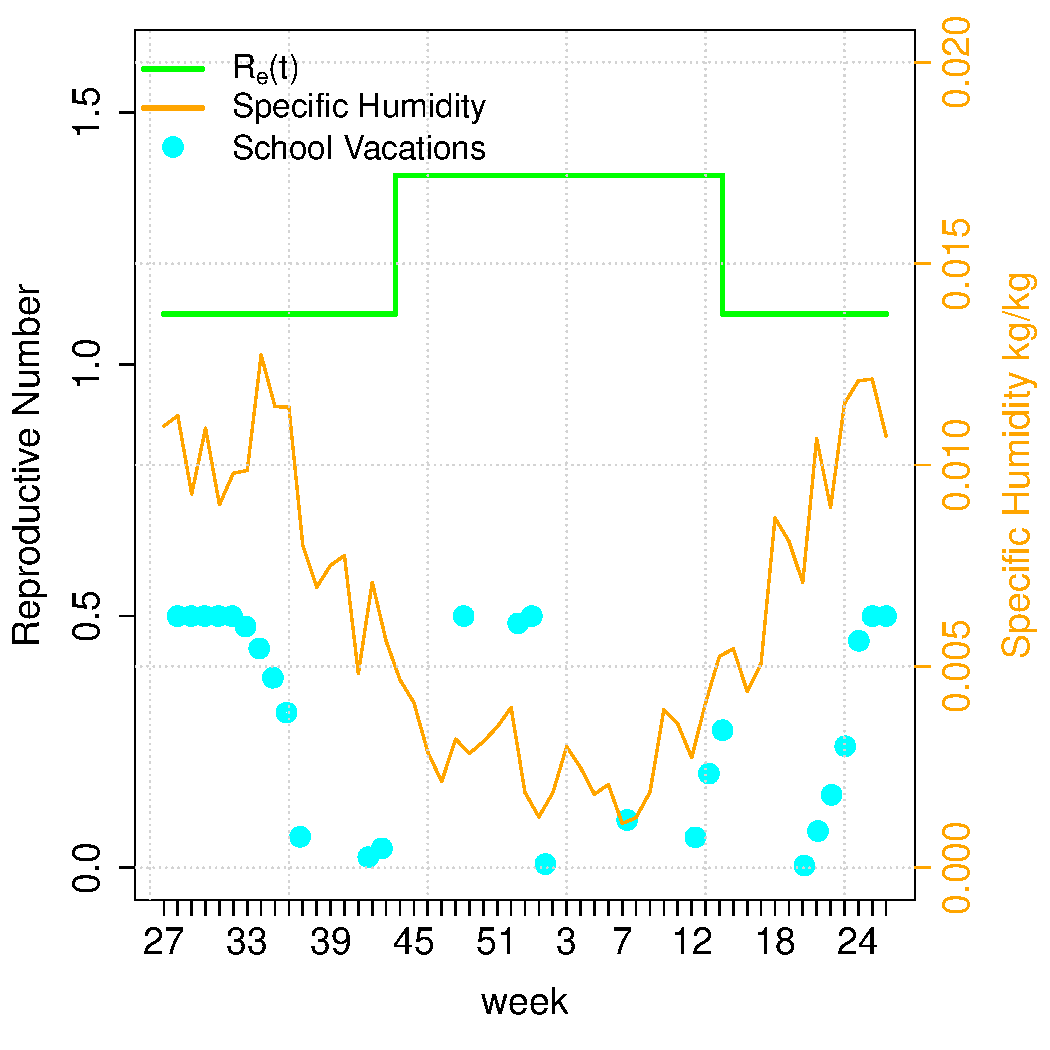
\includegraphics[width=2.7in]{figures/RoftModel5.pdf}
  \hspace{.1in}
  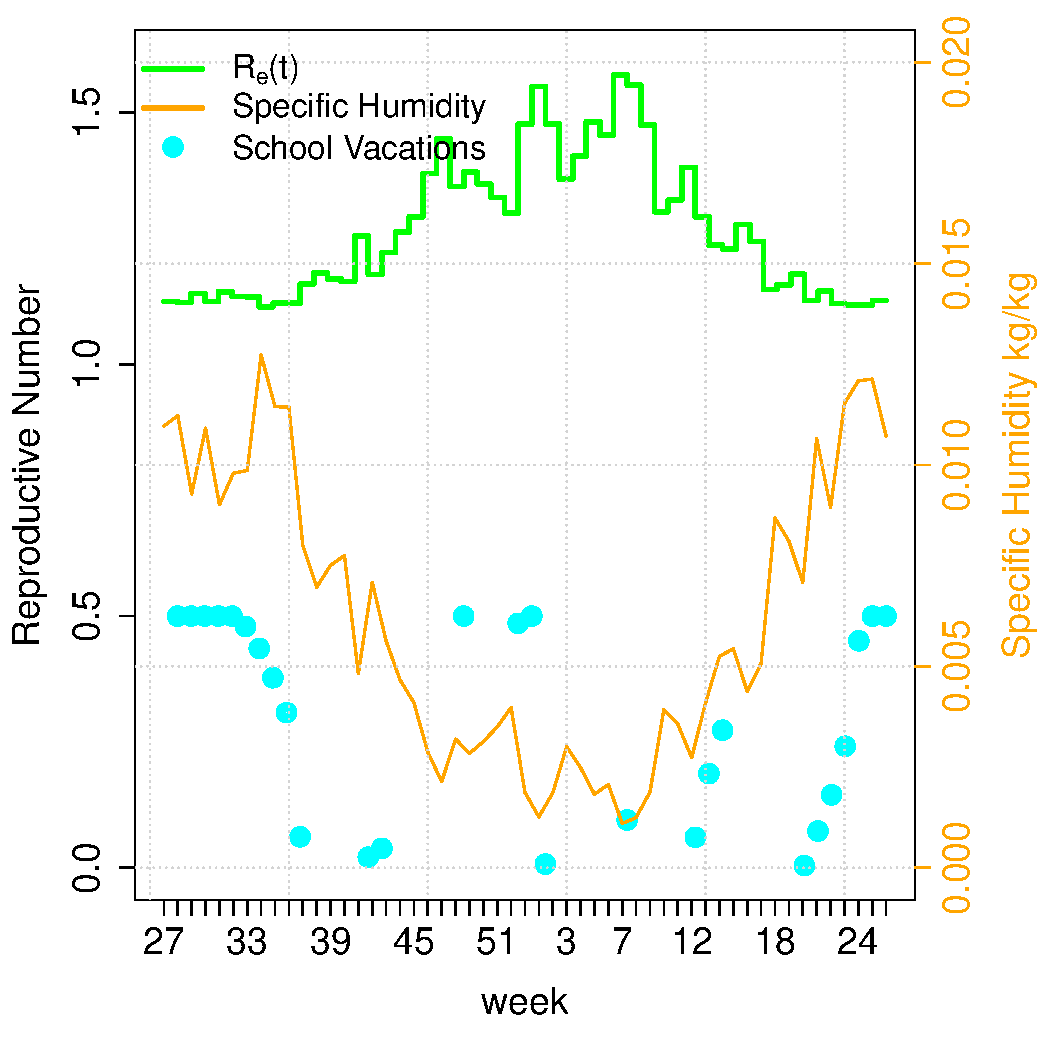
\includegraphics[width=2.7in]{figures/RoftModel3.pdf}
  \\[.1in]
  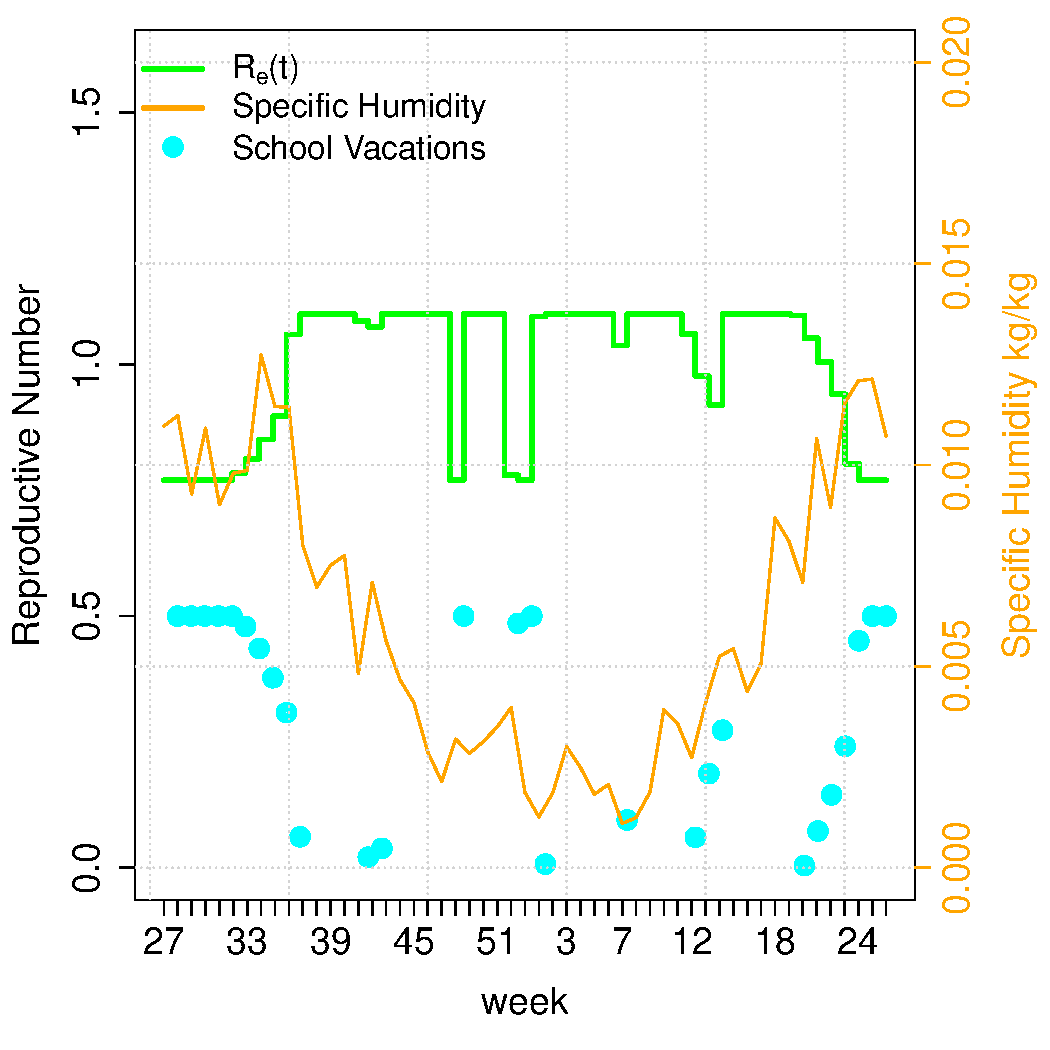
\includegraphics[width=2.7in]{figures/RoftModel2.pdf}
  \hspace{.1in}
  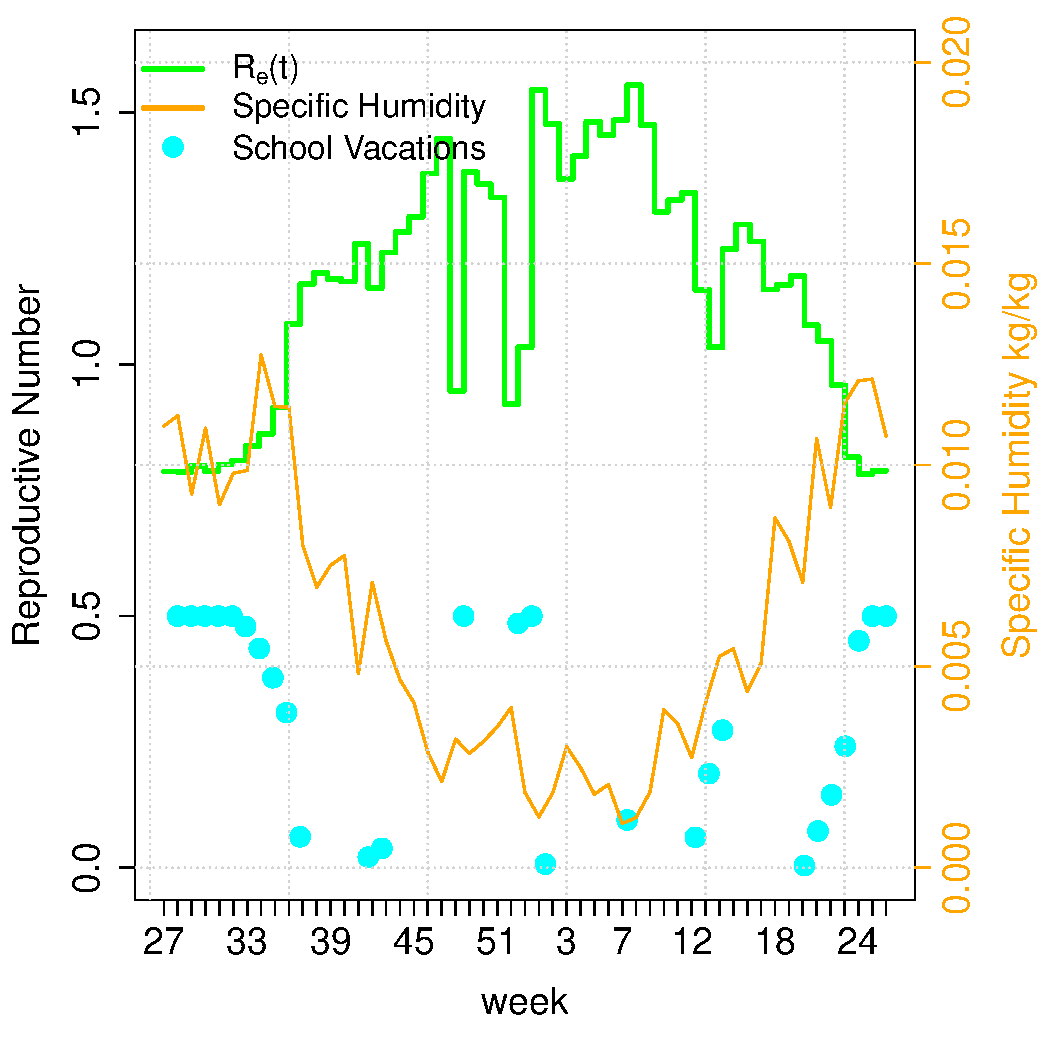
\includegraphics[width=2.7in]{figures/RoftModel1.pdf}
  \caption{$R_e(t)$ profiles for the model parameters: $R_{0}=1.1,\Delta_R=0.6,a=300,\alpha=0.3,t_s=18,dur=23,\Delta=0.25$. (Top Left) model 5: stepped-$R_e(t)$. (Top Right) model 1: specific humidity only.  (Bottom Left) model 2: school only. (Bottom Right) model 3: school and specific humidity terms.}
  \label{fig:Roft}
\end{figure}

A summary of the parameters recognized by the \pkg{DICE} package is found in table \ref{tab:param}.  The ``Optim Range" column is the range of values that the optimizer is allowed to vary over.  For the parameters that control $R_e(t)$, we show which model uses which parameters.  Both the default and range of values for the baseline parameter $B$ depend on $B_{est}$.  For a single flu-year (ex. Summer 2010--Summer 2011), $B_{est}$ is the average of the first five weeks of ILI data.
%\begin{table}[h]
%  \caption{\pkg{DICE} Model Parameters}
%  \centering
%  \begin{tabular}{|c|c|c|c|}
%    \hline
%    Parameter & Description & Default & Optim Range \\ \hline
%    $R_{0}$ & Baseline reproduction number & NA & 0.5--3.0 \\ \hline
%    $T_g$ & Average infectious period (default: $T_g=3$ days) & 3/7 & NA \\ \hline
%    $t_0$ & Infection start week & NA & 0.0--$nweeks/2$ \\ \hline
%    $I(t_0)$ & Initial number of infected & NA & 1--100 \\ \hline
%    $B$ & Baseline: mag. of non-SIR ILI data & $B_{est}$ & $(0.1*B_{est})$--$(10*B_{est})$ \\ \hline
%    $pC$ & Percent clinical & NA & $10^{-6}$--$1.0$ \\ \hline
%    $\alpha$ & Reduction in $R_e$ for school closed & 0 & $10^{-6}$--$1.0$ \\ \hline
%    $\Delta_R$ & Max change in $R_e$ from specific humidity & 0 & $10^{-6}$--$2.0$ \\ \hline
%    $a$ & Exponential for specific humidity $R_e$-term & 0 & 1--500 \\ \hline
%    $\Delta$ & Increase/Decrease in $R_e$ (model 5) & 0 & -1.0--1.0 \\ \hline
%    $t_s$ & Start time of change in $R_e$ (model 5) & 0 & 0--40 \\ \hline
%    $dur$ & time duration: $t_f=t_s+dur$ (model 5)& 0 & 0.01--40 \\ \hline
%  \end{tabular} \label{tab:param}
%\end{table}
\begin{table}[h]
  \caption{\pkg{DICE} Model Parameters}
  \centering
  \begin{tabular}{|c|c|c|}
    \hline
    Parameter & Description & Optim Range \\ \hline
    $R_\text{primary value}$ & Baseline reproduction number (models 1--5) & 0.5--3.0  \\ \hline
    $T_g$ & Average infectious period (default: $T_g=3$ days) & NA \\ \hline
    $t_0$ & Infection start week & 0.0--($nweeks/2)$ \\ \hline
    $I(t_0)$ & Initial number of infected & 1--100 \\ \hline
    $B$ & Baseline: mag. of non-SIR ILI data & $(0.1*B_{est})$--$(10*B_{est})$ \\ \hline
    $pC$ & Percent clinical & $10^{-6}$--$1.0$ \\ \hline
    $\alpha$ & Reduction in $R_e$ for school closure (models 2, 3) & $10^{-6}$--$1.0$ \\ \hline
    $\Delta_R$ & Max change in $R_e$ from specific humidity (models 1, 3) & $10^{-6}$--$2.0$ \\ \hline
    $a$ & Exponential for specific humidity $R_e$-term (models 2, 3) & 1--500 \\ \hline
    $\Delta$ & Increase/Decrease in $R_e$ (model 5) & -1.0--1.0 \\ \hline
    $t_s$ & Start time of change in $R_e$ (model 5) & 0--40 \\ \hline
    $dur$ & time duration: $t_f=t_s+dur$ (model 5)& 0.01--40 \\ \hline
  \end{tabular} \label{tab:param}
\end{table}

\subsection{Synthetic Examples}
To test the quality of both the coupled and uncoupled fitting procedures we provide a script that creates synthetic profiles (either coupled or uncoupled), fits them and compares the input and output values of all the parameters that were fitted.  For now, the code has been set up to work for Model number $4$ - a fixed value for the force of infection.

The script for the synthetic case is in the  `examples' directory: `example-synthetic.R'.  The script first sets all the parameters that the synthetic example expects and can not be changed. These are the $disease$, mod$\_$level and fit$\_$level which should be set to `flu', $2$ and $3$, respectively.  The year (i.e. flu season), is basically irrelevant (see below), and is simply set to $2015$. Then come the parameters that the user can change, with the two most important ones first:  coupled or uncoupled case and the number of MCMC steps (recommended value is $10^5$ or more). Other parameters include the plotting method, plotting device and sub-directory name for all the output files of the run.  The script loads the \pkg{DICE} package and uses all the chosen options to retrieve the `cdc' dataset for the 2015-2016 season: national and ten HHS regions.  Other run parameters are then set and the script calls the fitting routine (either coupled or uncoupled). In the fitting routine the real data for each of the ten HHS regions is replaced by synthetic data, created using either a coupled of uncoupled S-I-R model, with randomly chosen values for all the parameters of model $4$.  The national synthetic data is computed as a weighted average of the ten HHS regions. \pkg{DICE} then proceeds to fit the synthetic data using either the coupled or uncoupled procedure.   The output of the synthetic run (graphic files, csv files and binary RData files) is the same as that of a regular run with an additional graphic file showing the input values of the basic reproduction number, $R_0$, and the percent clinical, $pC$, for each of the ten HHS regions (in red vertical lines), along with their posterior densities from the MCMC chain. In the case of a coupled run we also show the input and densities of the two parameters that govern the coupling between regions: The saturation distance $s_d$, and the power $\gamma$ that determines the amount of mixing between regions (see also Equation \ref{eq:kappa}).  This additional graphic file has a unique name (see Section \ref{sec:output} for more details on the naming convention for files) which begins with the \textbf{FileType} `syn-'.


\section{Statistical Modeling}
\subsection{SARIMA Models}
\label{sec:sarima}

Whereas the main objective of \pkg{DICE} is to enable mechanistic modeling of (both direct and vector borne) epidemics on an arbitrary spatial scale with or without coupling between regions, it also supports statistical modeling that is based on Seasonal Autoregressive Integrated Moving Average (SARIMA) models.  These techniques are numerically fast but unlike the mechanistic model, described in detail in section \ref{sec:MechModeling}, it does not give us as much insight into the underlying physics of the disease.  For example, it can not tell us anything about the force of infection or the percent clinical.  But in some cases it can provide some information about the importance (or lack thereof) of multi-year seasonality. The selection of statistical vs. mechanistic modeling is determined by the key word `method' which can be set to either `stat' or `mech'.  When the SARIMA method is selected only a few parameters need to be set: (1) The user can select a specific SARIMA model by defining the `arima\_model' key word which is of type list (see below).  (2) If a specific `arima\_model' is selected the user can also select a covariate (key word `covar') and a (3) lag time for the covariate (key word `covar\_lag').

In general terms, SARIMA models can all be described as:

\begin{equation}
(p,d,q)(P,D,Q)_s
\end{equation}
where $p$ specifies the number of lags used in the model, $d$ represents the degree of differencing, and $q$ determines the number of error terms to include in the model. The next three parameters specify the ``seasonal'' aspects of the model, with $s$ being the length of the season (12 months or 52/53 weeks in our case).
For example, the selection $(1,0,0)(1,0,0)_{12}$ corresponds to a model that includes a non-seasonal autoregressive (AR) term of order one, a seasonal AR(1) term, no differencing, no moving average terms and a seasonal period of 12 months. Essentially, this is an AR model with predictors at lags of 1, 12, and 13 months. For each disease (and data source) \pkg{DICE} determines the length of the season (based on the temporal resolution of the data) hence the user need only define the $(p,d,q)(P,D,Q)$ values as a list, e.g.

\begin{verbatim}
> arima_model = list(p = 1, d = 0, q = 0, P = 1, D = 0, Q = 0)
> output <- runDICE(disease = 'dengue', data_source=NULL,
          year=2010, mod_level = 2, fit_level = 3, RegState = 'BR',
          method = 'stat', arima_model = arima_model)
\end{verbatim}


If the user does not provide a specific SARIMA model to \pkg{DICE} it is set to NULL and the code will use an automated process to select the best SARIMA model for each region (see next section for more details).  After selecting a SARIMA model the user can select as a covariate any of the climate data provided with \pkg{DICE}: temperature, specific humidity or precipitation (keyword `covar' set to `temp', `sh', or `precip', respectively).  In the case of the CDC ILI data, the user can also select the school vacation schedule as a covariate: `covar = school'.  By default, the covariate variable has a lag time of zero but this can be changed by setting the key word `covar\_lag' to `1' or `2' or more.  (The lag time has the same time units as the incidence data, e.g. week, month.)

\subsection{SARIMA Training and Forecasting}
When a statistical procedure is selected, with a specific SARIMA model, \pkg{DICE} first trains the model on (at most) the past ten years of incidence data (up to the latest available data point or the latest requested data point) and then uses the resulting parameters to make a forecast for the next 4 data points.  The statistical procedure can only be run in an uncoupled form and the logic of the procedure is identical to that of the mechanistic models.  Thus, the low resolution incidence data is first fitted and forecasted directly.  \pkg{DICE} then fits the high resolution data of each region/patch and these results are used with the proper weights to provide an indirect fit/forecast for the low resolution data. The resulting plots show the fits/forecasts of the high resolution incidence data along with the direct and indirect fits/forecasts of the low resolution data.
If the SARIMA model was defined by the user, the same model will be used in all of these fits along with the user  selected covariate and covariate lag time.  If however `arima\_model' is set to `NULL' \pkg{DICE} will use an automatic procedure to first train and then select the best SARIMA model for each (both high and low resolution) region.  This procedure, which is numerically more demanding, is pre-defined in \pkg{DICE} by setting upper limits on all the SARIMA model parameters and it does not allow the use of a covariate.


\section{DICE Data}
\label{sec:data}
The data incorporated into the \pkg{DICE} database includes incidence data across many diseases and countries, climate data derived from satellite imagery, population estimates, and school vacation schedules.  The following section details how data was collected and processed into the database.  Also included is an example of how to sift through the incidence data by location, disease, and/or data source.

\subsection{Incidence Data}
\label{sec:ILIData}
Incidence data was primarily collected from public-facing urls at country level Health Ministries.  A smaller fraction was collected from secondary sources including World Health Organization (WHO), Pan American Health Organization (PAHO), and manuscript supplementary information.  For best use with \pkg{DICE}, we focused on ingesting data reported monthly or higher cadence.  While there is some annual data in the database, it has generally been avoided.

A sampling of data sources are shown in table \ref{tab:data_sources}.  The complete table of data sources can be downloaded at anytime using a few lines of code:
\begin{verbatim}
> library(DICE)
> myDB = OpenCon()
> data_sources = dbReadTable(conn=myDB, name="data_sources")
\end{verbatim}
References in the full table contain a url when available as well as a semicolon delimited list of data columns.  For example, the RIO\_weekly data source has columns `cases' and `pop' indicating that this source contains both number of dengue cases and population for each region/sub-region and period in the dataset.  Similarly, the CDC source contains both percent ILI and number of ILI cases.
\begin{table}[h]
  \caption{Sample Data Sources}
  \centering
  \begin{tabular}{|l|c|c|r|c|}
    \hline
    Source & Disease & Source Abbv & Cadence & Col Names \\ \hline
    US-Centers for Disease Control & flu & CDC & 2 & ILI;cases  \\ \hline
    Brazil Ministry of Health & dengue & BRA\_MH & 3 & cases \\ \hline
    Rio Ministry of Health & dengue & RIO\_weekly & 2 & cases;pop \\ \hline
    Sri Lanka Ministry of Health & dengue & SRI\_monthly & 3 & cases \\ \hline
  \end{tabular} \label{tab:data_sources}
\end{table}
Cadence \#'s are explained in table \ref{tab:cadence} below.  The \textit{by-date} entry refers to data where each individual case is listed with a date.  Currently, \pkg{DICE} converts this type of data to daily totals (cadence=1) for fitting.
\begin{table}[h]
  \caption{Cadence Key}
  \centering
  \begin{tabular}{|c|c|}
    \hline
    Cadence \# & Cadence Desc \\ \hline
    0 & by-date \\ \hline
    1 & daily  \\ \hline
    2 & weekly \\ \hline
    3 & monthly \\ \hline
    4 & yearly \\ \hline
  \end{tabular} \label{tab:cadence}
\end{table}

The \pkg{DICE} database has too many data sources to include full descriptions here, but a few select sources are detailed below.

\subsubsection{CDC ILINet}
The CDC Influenza-like Illness surveillance Network (ILINet) Human and Health Services (HHS) region and national data were downloaded from the CDC-hosted web application FluView \url{http://gis.cdc.gov/grasp/fluview/fluportaldashboard.html}.  Figure \ref{fig:CDCregs} shows which states are grouped into each HHS region.  The circle in each region denotes the population density weighted location of the centroid of the region. The radius of each circle is proportional to the weight of the region which is determined by it's relative population (shown next to the centroid).


\pkg{DICE} is capable of downloading CDC ILI data using the R-package \pkg{cdcfluview}. This ensures that \pkg{DICE} is using the most up-to-date CDC data available.  If the data is temporarily unavailable, or cannot be accessed, \pkg{DICE} will use the data it has for the current season and notify the user that internal data, which may not be up-to-date, is used.  See the \textit{CDC\_server} flag in the `Data Selection Variables' below.
\begin{figure}[htbp]
  \centering
  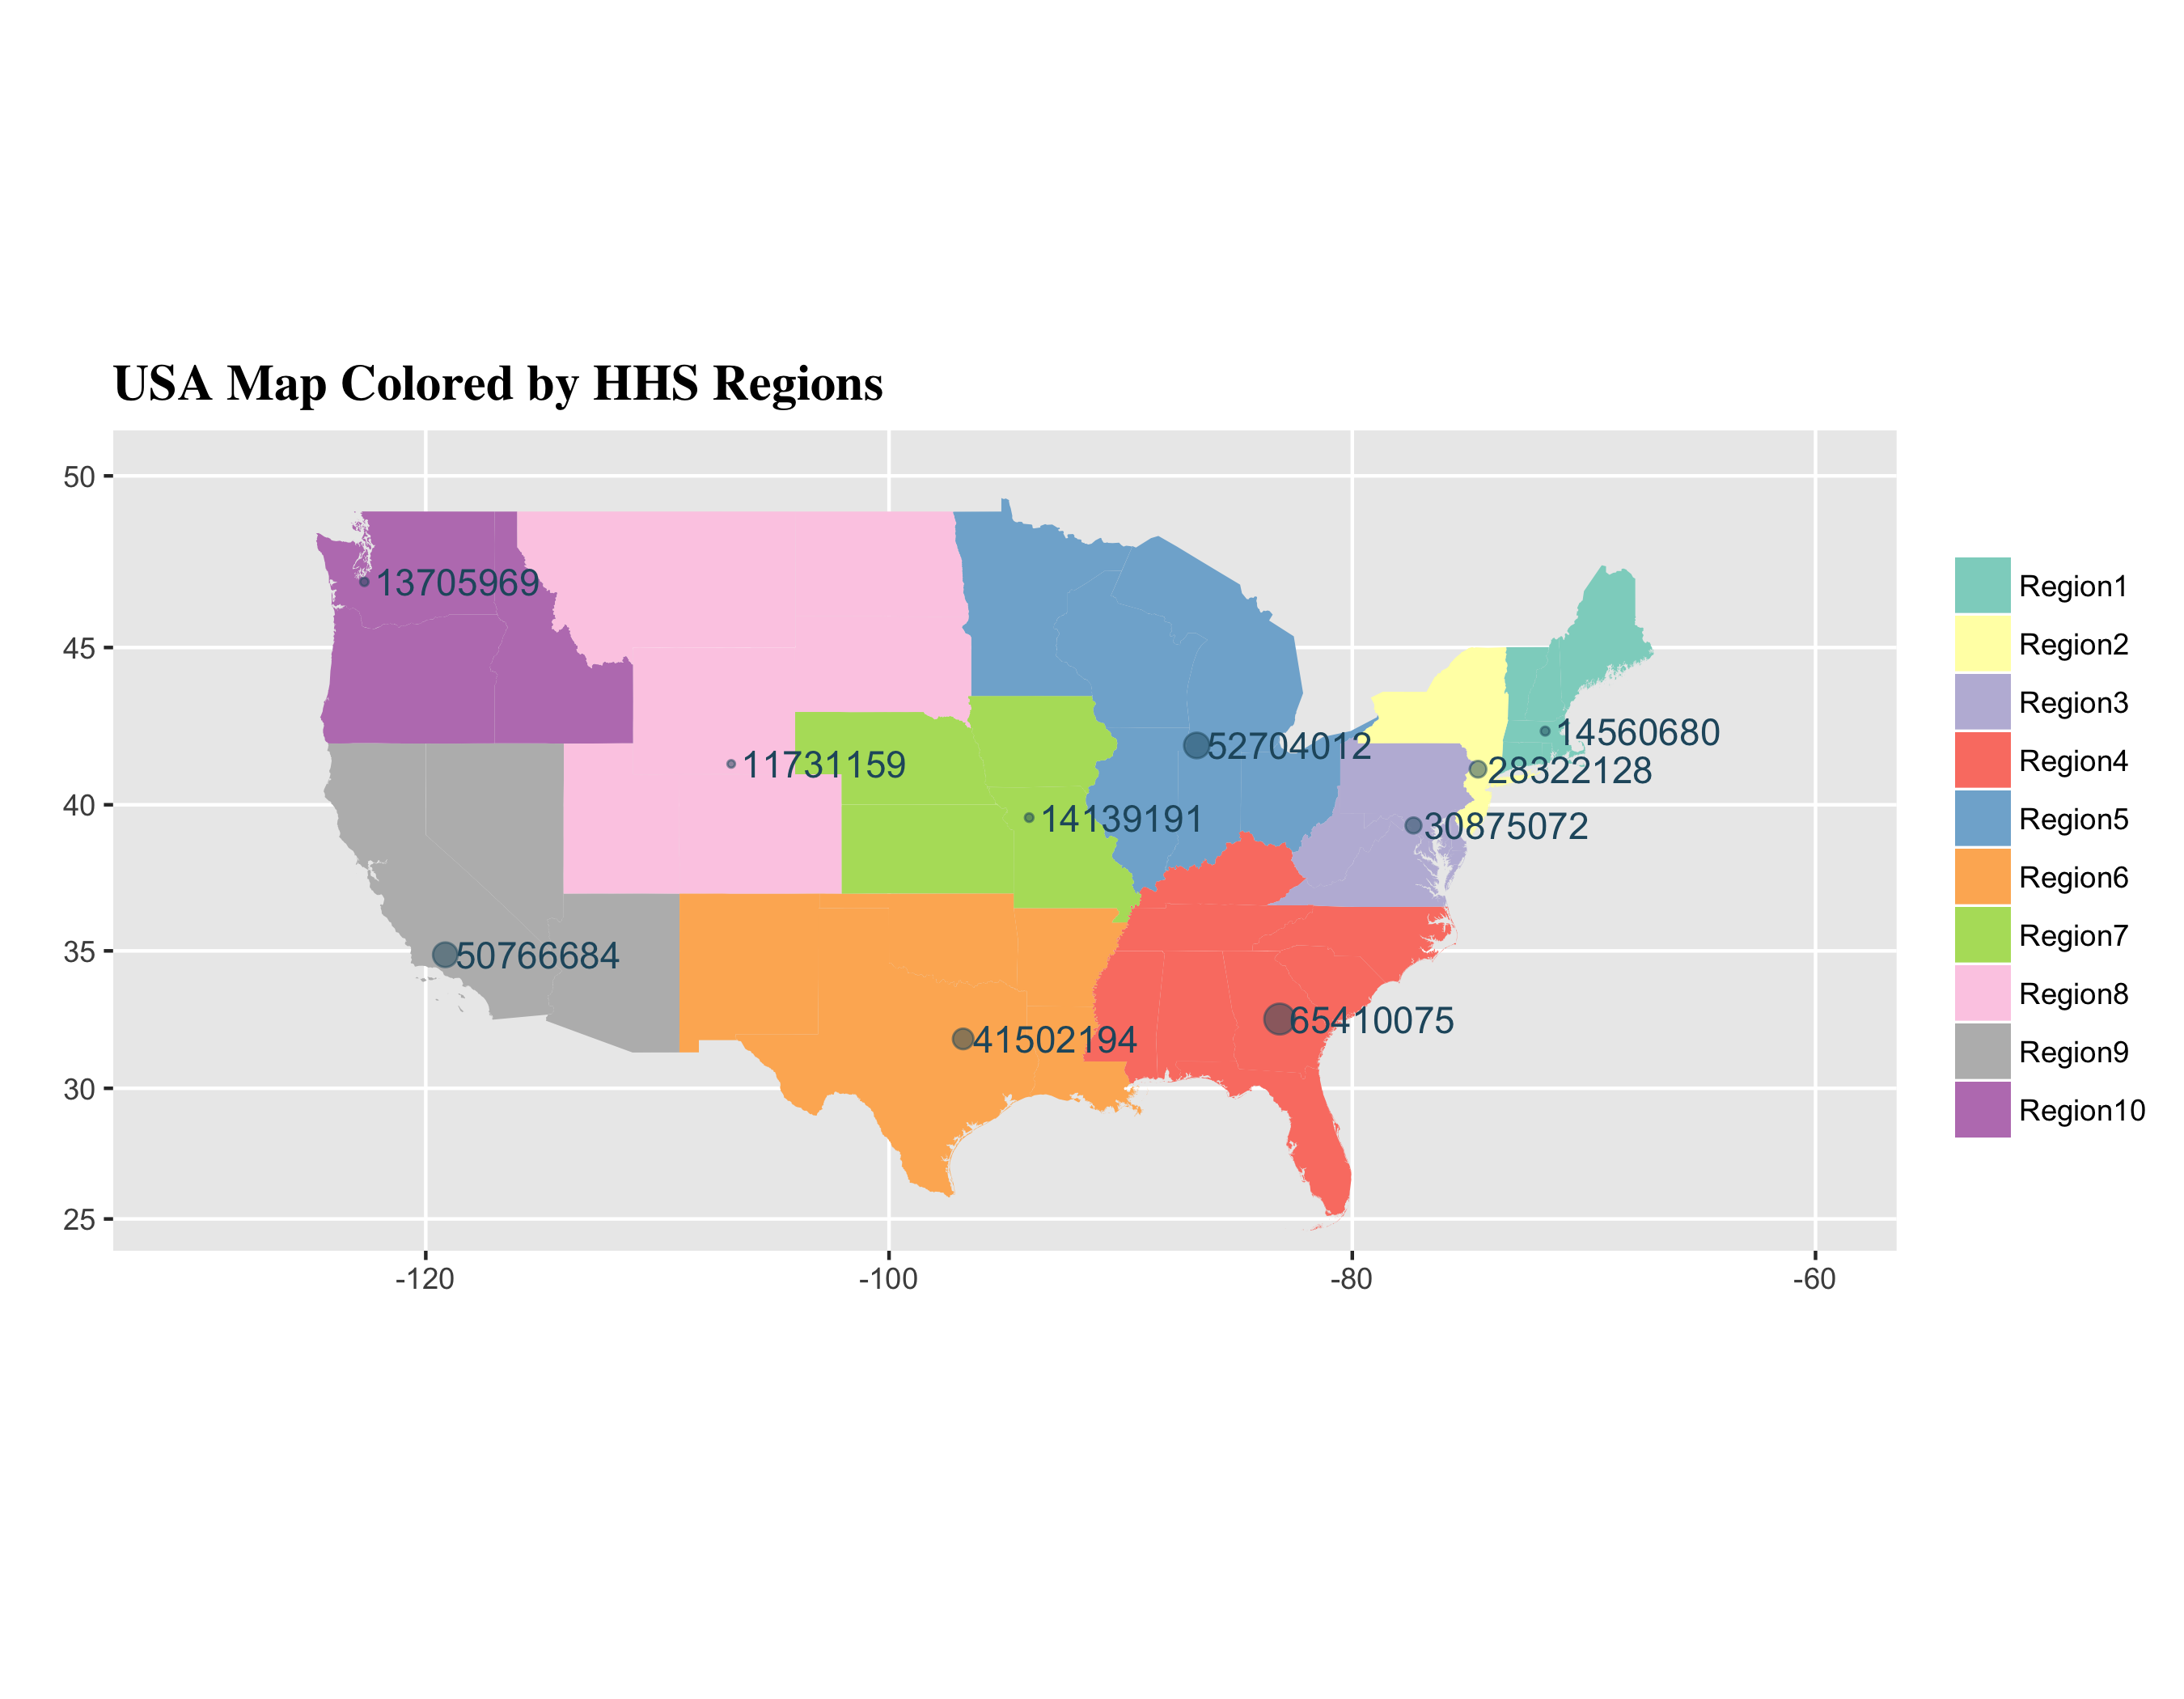
\includegraphics[width=4.0in]{figures/CDCRegions.png}
  \caption{CDC HHS Regions}
  \label{fig:CDCregs}
\end{figure}

The CDC Patient ILINet consists of more than 2,900 outpatient healthcare providers in all 50 states, Puerto Rico, the District of Columbia and the U.S. Virgin Islands reporting more than 30 million patient visits each year. Each week, approximately 2,000 outpatient healthcare providers around the country report data to CDC on the total number of patients seen and the number of those patients with influenza-like illness (ILI) by age group (0-4 years, 5-24 years, 25-49 years, 50-64 years, and $\geq65$ years). For this system, ILI is defined as fever (temperature of 100F or greater) and a cough and/or a sore throat without a \textit{known} cause other than influenza.  Sites with electronic health records use an equivalent definition as
determined by public health authorities.  The CDC Influenza surveillance data collection is based on a reporting week that starts on Sunday and ends on Saturday of each week.  With the exception of the 2009 influenza pandemic, each flu season starts on Week 27 and ends on Week 26 of the following year.  For 2009, the flu season started Week 13, 2009 (3-30-2009) and ended Week 26, 2010 (6-28-2010). For more information on ILINet see: \url{http://www.cdc.gov/flu/weekly/overview.htm}.

Because \pkg{DICE} requires an absolute number of incidents per week, CDC ILINet data is converted from percent ILI to approximate total ILI incidents.  We estimate the absolute number of weekly ILI cases by dividing the weighted percent of ILI cases in the CDC data (``X.WEIGHTED.ILI'' column) by 100 and multiplying it by the total weekly number of patients.  Total weekly patients is estimated as: (total population)*(2 outpatient visits per person per year)*(1 year/52 weeks).

We arrive at the estimate of 2 outpatient visits per year using two surveys published by the CDC: National Ambulatory Medical Care Surveys (NAMCS) \cite{namcs2011} and National Hospital Ambulatory Medical Care Surveys (NHAMCS) \cite{nhamcs2011}.  In the 2011 issues, the surveys estimated ambulatory visit rates of 3.32 visits per capita per year for Physician's offices, .43 for hospital emergency departments and .33 hospital Outpatient Departments.  We can sum these rates to get an outpatient visit per capita-year of 4.08. The rates for 2008 are 3.20, .41, and .37 respectively, which sums to 3.98 outpatient-visits per year.  In 2006 Schappert and Burt did a secondary study \cite{schappert2006} of the 2002 NAMCS and NHAMCS reports and calculated an ambulatory rate of 3.8 visits per capita-year. We further estimate from the surveys that approximately one half of outpatient visits are at a medical practice who's specialty is ineligible for ILINet participation.  Thus we arrive at the estimation (4 outpatient visits per capita-year)*(1 ILI-reportable visit/2 visits) = 2 ILI-reportable visits per capita-year.  By incorporating this best-estimate, we hope to improve the accuracy of $p_C$ posteriors.

\subsubsection{Google Flu Trends}
Google Flu Trends data (at the national, state and city level) was obtained directly from the GFT web site: \url{http://www.google.org/flutrends/us/data.txt}. GFT attempts to quantify ILI cases through a proprietary model using key terms from search queries (originally discussed in \cite{ginsberg2009}; see also \cite{cook2011, copeland2013}).  GFT ILI estimates were publicly accessible from Week 39, September 28th, 2003 to Week 32, August 9th, 2015. The GFT data is aggregated to the same ten HHS regions as for the CDC data and the flu seasons were also defined using the same dates.  In addition, some of the GFT data is available at state levels.  To create a state-level dataset that spans all available years, the GFT data in \pkg{DICE} consists of two different GFT model updates.  The 2003-2013 flu seasons are covered by GFT data from the 2013 model-update.  Then the 2014-2015 season is covered by GFT data from the 2014 model-update.
%In addition to the original GFT data, \pkg{DICE} now includes the 2014 model revision update, referred to as: GFT$^+$, see: \url{https://www.google.org/flutrends/historic/us-historic-v3.txt}.  The GFT$^+$ data set is limited to the national and HHS regions level.   For more information on GFT and GFT$^+$, see: \url{http://www.google.org/flutrends/about/how.html}.

\subsubsection{AFHSC Flu Incidence}
The Military data (data\_source=`AFHSC') was obtained from the Armed Forces Health Surveillance Center (AFHSC) consisting of outpatient visits to permanent military treatment facilities (MTFs) by active duty military personnel for a range of International Classification of Diseases (ICD)-9 codes associated with respiratory-related illnesses between January 1, 2009 and April 30, 2011.  For each record, the data contained: a unique study identifier for the individual; ICD-9 codes associated with that visit; and the zip code (5 digits) of the clinic location.  We use the zip code of the reporting clinic as a proxy with which to define a military installation: we do not explicitly represent military installations or bases, rather, we assume that the case reports from the same zip code are from the same military installation.  Each record (an anonymized Study ID) was assigned as either ``ILI-large'' ($n=1,336,471$)  or ``ILI-small'' ($n=27,582$) using a set of classifications based on ICD-9 codes \cite{riley13a}. The definition of ILI-large was broader and included non-specific diagnosis such as: `viral infection' and `acute nasopharyngitis'. The definition of ILI-small was more constrained and included: `influenza w/other respiratory manifestations' ($n=25,293$), `influenza with manifestation not elsewhere classified (NEC)' ($n=1,006$), `infectious upper respiratory, multiple sites, acute NEC' ($n=897$), and `influenza with pneumonia' ($n=404$).  We further trimmed the data temporally to cover the period from April 1, 2009 through June, 1, 2010 which is the 2009 H1N1 pandemic period.  We ranked the military installations by size according to the total number of ILI-small cases they reported. In the \pkg{DICE} database we provide the data for the top-50 largest profiles, 47 of which, were located within the USA.  Of the remaining three, one was located in Landstuhl, Germany, and two were located in Japan (Misawa and Yokosuka).



\subsection{Climate Data}
In every geographic region for which the \pkg{DICE} database has incidence data, climate data is automatically pre-calculated.  Generally this consists of temperature, precipitation, and specific humidity processed from data generated by the National Oceanic and Atmospheric Administration's (NOAA) National Centers for Environmental Prediction (NCEP)/National Center for Atmospheric Research (NCAR) Reanalysis-2 project. This data is processed to a single population-weighted value for each region at a cadence of daily/weekly/monthly to match the cadence of incidence reporting.

Additionally, specific humidity is tracked for the contiguous United States using the National Atmosphere and Space Agency's (NASA) North American Land Data Assimilation System (NLDAS)-2 dataset. This is legacy code that does not incorporate population-weighting.

\subsubsection{NOAA Climate Data}
NOAA's NCEP/NCAR Reanalysis-2 project \cite{kalnay1996ncep} (see for example: \url{http://iridl.ldeo.columbia.edu/SOURCES/.NOAA/.NCEP-NCAR/.CDAS-1/.DAILY/.Diagnostic/.above_ground/.qa/}) provides climate data 4-times daily, on a spatial grid of $2.5^{\circ}$ for the entire world from 1979-present (2 week to 2 month lag).  The original grid is first averaged to daily values.  Then the Database of Global Administrative Areas (GADM) is used to define boundaries while Socioeconomic Data and Applications Center (SEDAC) maps are used to approximate population distributions.  By overlaying GADM boundaries on both the Reanalysis-2 and SEDAC grids, \pkg{DICE} is able to calculate a population-weighted daily climate time-series for each region.  Currently, \pkg{DICE} expects the climate variables on the same cadence as the incidence data, so the daily climate data is averaged to weekly/monthly/yearly wherever weekly/monthly/yearly incidence exists.

\subsubsection{NASA Specific Humidity}
Our secondary source of specific humidity is calculated from the NLDAS-2 database published by NASA \url{http://ldas.gsfc.nasa.gov/nldas/NLDAS2model.php/} \cite{xia2012continental,mitchell2004multi}. The NLDAS-2 database provides hourly specific humidity (measured 2-meters above the ground) for the continental US at a spatial grid of $0.125^{\circ}$ which we average to daily and weekly SH. The weekly data is then spatially-averaged for the states and CDC regions.  Because they are not covered by the NLDAS grid, Alaska and Hawaii always use specific humidity from the NOAA Reanalysis dataset.

\subsection{School Vacation Schedules}
Currently school vacation schedules have been collected only for the United States.  For each state, school vacation schedules were approximated by averaging the public school vacation schedule from the three largest cities in that state for the 2014-15, 2015-16, and 2017-2018 school years.  Approximations for region schedules are determined by a population-weighted average of state schedules.  The same process is then applied to the regions to recover a national school schedule.  The value of $p(t)$ represents school closures in a state/region for the week $t$. Based on the proportion of schools closed and number of days closed, $p(t)$ is assigned a value in the range $[0,1]$.  For example in week $t_i$, if all schools are closed for the entire week then $p(t_i)=1$.  However, if all schools have Monday and Tuesday off (missing 2 of 5 days), then  $p(t_i)=0.4$.  Similarly, if 3 of 10 schools have spring break (entire week off), but the other 7 schools have a full week of class then $p(t_i)=0.3$.  And of course if all schools have a full week of class then $p(t_i)=0$.

For the Military data we were able to find school schedules for only some of the military bases (using the school district they belong to). This information was then used to create an approximate school schedules for all 50 bases.  Note that, given the timing of the 2009-2010 H1N1 pandemic, we do not expect school vacations to play an important role in this case.


\subsection{Population Data}
Population data has been collected from census bureaus, incidence data, and GADM/SEDAC overlay.  In this context `incidence data' refers to incidence reports that include a population estimate as an auxiliary value to the number of cases.  For example the Rio de Janeiro Health Department dengue reports divide the municipality into ~200 regions/sub-regions, each of which contains a yearly population estimate (ex. http://www.rio.rj.gov.br/web/sms/exibeconteudo?id=2815389).  The third type of population data is computed by overlaying GADM administrative boundaries on the SEDAC population density map.  In this way, we can produce a population estimate for any region of the world that is defined in GADM or can be represented as a collection of sub-regions that are defined in GADM. When retrieving population data for \pkg{DICE}, sources are prioritized in the following order: (1) auxiliary incidence data (2) census data (3) GADM/SEDAC.

% Denominator civilian data was obtained from the US 2010 census data
% center: \url{http://www.census.gov/2010census/data/}.  The estimated
% inter-censal state and national population sizes between 2000 and 2010
% were obtained from
% \url{http://www.census.gov/popest/data/intercensal/state/state2010.html}
% and  \url{http://www.census.gov/popest/data/intercensal/state/tables/ST-EST00INT-01.csv}.
%
% The projected state and national population sizes from 2010-2015 were
% obtained from \url{http://www.census.gov/popest/data/datasets.html}
% and  \url{http://www.census.gov/popest/data/state/totals/2015/tables/NST-EST2015-01.csv}.
% Each region population size was calculated by summing the population sizes of every state in the region.


For the Military data, we provide our estimate of the total population ($N_{total}$), the ``denominator data'', for each of the 50 military installations.
Our method for estimating these sizes relied on the use of the total number of visits to a clinic for all causes as a proxy for the total number of active duty personnel at that location. The
coefficient of proportionality $\Omega$ was estimated by using a subset of the installations for which reasonably reliable estimates for the total population have been published.


\subsection*{DICE Data Structure}
The \pkg{DICE} dataset is structured to organize global disease incidence data on a multitude of spatial scales.  An important aspect of the data structure organization is the idea of spatial `levels'. The levels for the United States are defined as seen in table \ref{tab:levels} . Levels 3 and up are likely to be labeled differently in each country.  For example, the levels in Australia are labeled as: 3-State/Territory, 4-Health Region, 5-Local Governing Unit, 6-City.

\begin{table}[h]
  \caption{Population levels}
  \centering
  \begin{tabular}{| c | l |}
    \hline
    Level & Description \\ \hline
    0 & Global \\ \hline
    1 & Continent \\  \hline
    2 & Country \\  \hline
    3 & HHS Region \\  \hline
    4 & State \\ \hline
    5 & County \\ \hline
    6 & City \\ \hline
  \end{tabular}
  \label{tab:levels}
\end{table}

A common application of \pkg{DICE} is to use the characteristics of sub-population profiles to build an epidemic forecast for the population of interest.  For example one might analyze the 50 states (coupled or uncoupled) to recover a more accurate national forecast.  For this purpose we have defined \textit{fit level} as the population level that is being fit and \textit{model level} as the level to be modeled/forecast.  The model-level population may be a previously defined country/region or the user may select regions/states to define a new country/region with.  See the description of \textit{fit\_name} below for more information about creating a new region.

\subsubsection*{Data Selection Variables}
The function \textit{get.DICE.data}() provides easy access to all data in the \pkg{DICE} database.  Whether the data is accessed directly through \textit{get.DICE.data}() or simply by use of \textit{runDICE}(), the list below provides useful descriptions of the input variables.

 \textbf{data\_source} - A string or integer specifying the data source. See section \ref{sec:ILIData} about accessing the \textit{source\_abbv} column of the data\_sources table. Additionally, the \pkg{DICE} functions \textit{SummaryByCountry}() and \textit{SummaryBySource}() are quite useful for determining source abbreviation.

 \textbf{mod\_level} - An integer value indicating the population-level of the incidence profile to model/forecast.  Table \ref{tab:levels} shows the population levels for the United States.  Levels 3+ may vary by country.  For example the levels in Australia could be defined as: 3-State/Territory, 4-Health District, 5-Local Government Area, 6-City.

 \textbf{mod\_name} - A named vector of strings specifying the model-level spatial patch.  If \verb|is.null(mod_name)|, the code reverts to using \textit{RegState} (see next entry).  To specify New York state, set \verb|mod_name=c(NAME_2="United States", NAME_3="R1", NAME_4="New York")|. Here \textit{NAME\_X} is either the full name or abbreviation of the level-X patch. Replacing `United States' with `US' or `R1' with `Region 1' would result in the same outcome.  Also, vector entries for \textit{mod\_name} should go from \textit{NAME\_2},\ldots, \textit{NAME\_n} where \textit{mod\_level}=n.

 \textbf{RegState} - Determines which single region from \textit{mod\_level} is to be modeled.  This is a legacy input that is limited to countries and United States regions/states.  \textit{mod\_name} is the more robust input.  Depending on the model level, \textit{RegState} should adhere to the following format: \textit{mod\_level} = 2 - 3-letter ISO3 country code, \textit{mod\_level}=3 - an integer describing the HHS region, \textit{mod\_level}=4 - a 2-letter state code.

 \textbf{fit\_level} - An integer value indicating the population-level of the incidence profile(s) to be fit.  \textit{fit\_level} $\geq$ \textit{mod\_level}.  See table \ref{tab:levels}. It is possible to run \pkg{DICE} for a single population by choosing $mod\_level=fit\_level$.  This indicates to \pkg{DICE} that the \textit{model} region is to be fit directly with no higher-level indirect fits.

 \textbf{fit\_names} - If \textit{fit\_names}==``all", then all regions at \textit{fit\_level} that are children of \textit{mod\_name} will be used.  Otherwise, \textit{fit\_names} should be a vector of strings specifying the names or abbreviations to construct a region from.  For example, if we wanted to construct a Pacific Coast Region for the contiguous United States we would use the inputs: \textit{mod\_level}=2, \textit{mod\_name}=``US", \textit{fit\_level}=4, and \textit{fit\_names}=\verb|c("CA", "OR", "WA")|.

 \textbf{year} - Integer specifying the season year. Default season start and end dates are stored in the \textit{season\_se\_dates} table in the database.

 \textbf{disease} - String describing the which disease.  See section \ref{sec:ILIData} about accessing the \textit{disease} column of the data\_sources table.

 \textbf{db\_opts} - A list of database options.  The \textit{DICE\_db} option determines which SQL database to retrieve data from `PredSci' or `BSVE'.  The \textit{CDC\_server} option determines if incidence data should be retrieved directly from CDC servers.  \textit{CDC\_server} should be set to TRUE only when \textit{data\_source}= `cdc' or 7.


\subsubsection*{Data Lookup}
To get a snapshot of the incidence data currently available in the \pkg{DICE} database, use the functions SummaryByCountry() and SummaryBySource().  Following the example below, it becomes straightforward to determine which dataset you would like to use and fill the \textit{disease} and \textit{data\_source} inputs.  SummaryByCountry() is focused on summarizing the spatial levels of data by country, while SummaryBySource() breaks-down each country/disease pair by the data sources.  The data structure returned by SummaryByCountry() is ordered by disease/country/cadence.  The output from SummaryBySource() is ordered as disease/country/root-location/data\_source.

The complete list of data sources (when this document was compiled) is seen in Table \ref{tab:sources} below.
% latex table generated in R 3.3.0 by xtable 1.8-2 package
% Thu Jan 17 12:44:13 2019
\begin{table}[ht]
\centering
\caption{Complete list of DICE database data-sources as of 2019-01-17.} 
\label{tab:sources}
\begin{tabular}{|r|l|l|l|}
  \hline
source\_key & source\_abbv & disease & source\_desc \\ 
  \hline
  1 & BRA\_MH & dengue & Brazil national epidemiological data system ( \\ 
    2 & RIO\_monthly & dengue & Municipality of Rio de Janeiro Health departm \\ 
    3 & RIO\_weekly & dengue & Municipality of Rio de Janeiro Health departm \\ 
    4 & Sri\_monthly & dengue & Sri Lanka Ministry of Health: Epidemiology Un \\ 
    5 & Sri\_weekly & dengue & Sri Lanka Ministry of Health: Epidemiology Un \\ 
    6 & MEX\_portal & dengue & Mexico Federal Government portal \\ 
    7 & CDC & flu & United States Centers for Disease Control ILI \\ 
    8 & TYCHO & dengue & TYCHO-University of Pittsburgh  \\ 
    9 & THA\_MH & dengue & Thailand Ministry of Health - Weekly Epidemio \\ 
   10 & USA\_SD & flu & San Diego County - Influenza Watch \\ 
   11 & USA\_TN & flu & Tennessee Department of Health - Sentinel Sur \\ 
   12 & SGP\_MH & dengue & Singapore Ministry of Health - Epidemiologica \\ 
   13 & SAU\_MERS & mers\_cov & Saudi Arabia MERS reporting \\ 
   14 & SARS\_2003 & sars & Country-level SARS incidence \\ 
   15 & WHO\_flu & flu & WHO influenza incidence at country level and  \\ 
   16 & SOM\_MH & cholera & Somalia Ministry of Health \\ 
   17 & ZMB\_MH & cholera & Zambia Ministry of Health \\ 
   18 & WHO\_chlr & cholera & World Health Organization - annual cholera \\ 
   19 & BRA\_yf & yellow\_fever & Brazil Ministry of Health yellow fever \\ 
   20 & TWN\_den & dengue & Taiwan CDC \\ 
   21 & CA\_meas & measles & California measles reporting \\ 
   22 & FSM\_meas & measles & Micronesia 2014 measles outbreak \\ 
   23 & JAM\_chik & chik & Jamaica Data Portal \\ 
   24 & MDG\_plag & plague & Ministry of Health of Madagascar \\ 
   25 & And\_Lab & zika & Anderson Lab Digitization of PAHO records \\ 
   26 & quidel & flu & private \\ 
   27 & WHO\_ebo & ebola & WHO weekly ebola \\ 
   28 & COD\_ebol & ebola & A Rosello - eLife 2015, Ebola linelist \\ 
   29 & CDC\_lyme & lyme & CDC Monthly Average National Cases \\ 
   30 & CDC\_deng & dengue & CDC Monthly Dengue reporting for American Sam \\ 
   31 & siraj\_zika & zika & Siraj et al, Zika in Colombia, hosted on Drya \\ 
   32 & idn\_dengue & dengue & "Prediction of Dengue Outbreaks based on Dise \\ 
   33 & isr\_meas & measles & Israel Ministry of Health \\ 
   34 & nga\_lassa & lassa & Nigeria Centre for Disease Control \\ 
   \hline
\end{tabular}
\end{table}
\clearpage % Force the table to be placed ahead of the examples below.  This may result in an odd-lookin pagebreak.

Example of looking-up data for dengue in Brazil
\begin{verbatim}
  > library(DICE)
  > test = SummaryByCountry()
  > test$dengue$brazil$tot_regions
  [1] 5702
  > test$dengue$brazil$RegionsByLevel
    level num_regions
  1     2           1
  2     3           5
  3     4          27
  4     5        5467
  5     6          11
  6     7          31
  7     8         160
  > test$dengue$brazil$Weekly
    level num_regions   min_date   max_date
  1     5           1 2000-01-02 2018-02-11
  2     6          11 2000-01-02 2018-02-11
  3     7          31 2000-01-02 2018-02-11
  4     8         160 2000-01-02 2018-02-11
\end{verbatim}

Example 2 looking-up data for dengue in Thailand
\begin{verbatim}
  > test = SummaryBySource()
  > test2$dengue$Thailand$Thailand$THA_MH
  $source_info
    source_key cadence disease
  9          9       3  dengue
                                           source source_abbv
  9 http://www.wesr.moph.go.th/wesr_new/index.php      THA_MH
                                                                 source_desc
  9 Thailand Ministry of Health - Weekly Epidemiological Surveillance Report
    data_cols col_names                 col_units bsve_use countries
  9         2 cases;pop reported cases;population        1        TH
    max_lev min_lev
  9       5       2

  $data_summary
    levels num_regions   min_date   max_date
  1      2           1 2007-01-01 2017-12-01
  2      3           4 2007-01-01 2017-12-01
  3      4          13 2007-01-01 2017-12-01
  4      5          77 2007-01-01 2017-12-01
\end{verbatim}
From looking through the output of SummaryBySource() we see that we want to set disease=`dengue' and data\_source=`THA\_MH'.  Now if we do not already have a region to model in mind, we can search through the regions by first grabbing the dengue lookup table.
\begin{verbatim}
  > myDB = OpenCon()
  > dengue_lut = dbReadTable(conn=myDB, name="dengue_lut")
  > dbDisconnect(myDB)
\end{verbatim}
Say we want to look at health zones (level 4) in Thailand.  A list of level 4 names can be returned by:
\begin{verbatim}
  > dengue_lut$NAME_4[dengue_lut$level==4 & dengue_lut$NAME_2=="Thailand"]
   [1] "Zone 1"       "Zone 2"       "Zone 3"       "Zone Bangkok"
   [5] "Zone 4"       "Zone 5"       "Zone 6"       "Zone 7"
   [9] "Zone 8"       "Zone 9"       "Zone 10"      "Zone 11"
  [13] "Zone 12"
\end{verbatim}
Lets say we want to model Zone 5 using its provinces.  If we want a list of provinces in Zone 5
\begin{verbatim}
  > dengue_lut$NAME_5[dengue_lut$NAME_2=="Thailand" & dengue_lut$NAME_4=="Zone 5" &
               dengue_lut$level==5]
  [1] "Ratchaburi"          "Kanchanaburi"        "Suphan Buri"
  [4] "Nakhon Pathom"       "Samut Sakhon"        "Samut Songkhram"
  [7] "Phetchaburi"         "Prachuap Khiri Khan"
\end{verbatim}
The next step is to return the lookup table row corresponding to Zone 5 so we know how to fill \textit{mod\_name}.
\begin{verbatim}
  > dengue_lut[dengue_lut$NAME_2=="Thailand" & dengue_lut$NAME_4=="Zone 5" &
               dengue_lut$level==4, ]
        identifier level NAME_1   NAME_2         NAME_3 NAME_4 NAME_5
  5954 AS.TH.R2.Z5     4   Asia Thailand Central Region Zone 5   <NA>
       NAME_6 NAME_7 NAME_8 ID_1 ID_2 ID_3 ID_4 ID_5 ID_6 ID_7 ID_8
  5954   <NA>   <NA>   <NA>    3  228    2    5   NA   NA   NA   NA
       ABBV_1 ABBV_2 ABBV_3 ABBV_4 ABBV_5 ABBV_6 ABBV_7 ABBV_8 inc_key
  5954     AS     TH     R2     Z5   <NA>   <NA>   <NA>   <NA>      55
       master_key gadm_name gadm_lvl  clim_ident gadm_noaa_sedac_ident
  5954   22800055      <NA>       NA AS.TH.R2.Z5                  <NA>
       gadm_lat gadm_lon gadm_area sedac_lat sedac_lon sedac_pop
  5954 13.81896 99.44633  45946.85   13.6808  99.90137   5817362
\end{verbatim}
From this information we can now define \textit{mod\_name}=\texttt{c(NAME\_2="Thailand", NAME\_3="Central Region", NAME\_4="Zone 5")}, \textit{mod\_level}=4, and \textit{fit\_names}=\verb|"all"|


\subsubsection*{Week Indexing}
To be consistent with week numbering and dates, we have adopted the CDC/MMWR week numbering system.  This means that a week begins on Sunday and ends on Saturday.  For the purpose of numbering weeks of a year this dictates that week number 1 is the week containing the first Wednesday of the year.  Any January days occurring before week 1 are considered part of the final week (52 or 53) of the previous year (\url{https://wwwn.cdc.gov/nndss/document/MMWR_week_overview.pdf}).

\section{Mechanistic Models: Fitting Procedure}
\label{sec:FittingProcedure}
The \pkg{DICE} incidence fitting procedure determines the joint posterior
distribution for the model parameters using a Metropolis-Hastings Markov
Chain Monte Carlo (MCMC) procedure \cite{gilks96a}.  It should be stressed that although we often refer to the MCMC algorithm in the context of an optimizer, it is better characterized as a probability distribution mapping routine.  As such, the random walk will likely spend the majority of its time in the neighborhood of the optimal (most likely) solution.  However it's purpose is to find a distribution of most-likely solutions, not necessarily \textit{the} best solution.

After the user selects a compartmental model, and a model number for $R_e(t)$ (which triggers \pkg{DICE} to set TRUE/FALSE values for parameters that need/not be optimized), the user needs to tell \pkg{DICE} how
many MCMC chains to run and how many steps to take in each
chain. \pkg{DICE} will then randomly initialize the parameters that are
optimized (using a log-uniform distribution for all the parameters
except the one that can be negative) integrate the coupled equations (S-I-R, S-E-I-R etc.) and
incidence equations and generate a candidate incidence profile. The
likelihood of this solution is calculated using the Akaike Information Criterion (AIC), which is a measure of the relative goodness of fit of a model:

\begin{equation}
{\rm AIC} = -2 \log (L(\hat{\theta}| I_C)) + 2 K
\label{eq-aic1}
\end{equation}
where $\log (L(\hat{\theta} | I_C))$ is the value of the maximized log-likelihood over the model parameters ($\theta$), given the observed cases $I_C$.
When the total number of parameters ($K$) is large relative to the sample size ($n$), the reduced Akaike Information Criterion is preferred:

\begin{equation}
{\rm AIC}_c = -2 \log (L(\hat{\theta})) + 2 K + \frac{2 K (K+1)}{(n - K - 1)}
\label{eq-aic2}
\end{equation}
and this is what \pkg{DICE} uses.   The log-likelihood stems from a Poisson probability density
\begin{equation}
  \log (L(\theta| I_C)) = \sum_i w_i \Big(I_C(t_i)\cdot \log\big(I_R(t_i,\theta)\big) - I_R(t_i,\theta) - \log\big(I_C(t_i)!\big) \Big)\;,
  \label{eq-wLLK}
\end{equation}
where $I_R(t_i,\theta)$ is the model point generated for week $t_i$ as a result of parameter set $\theta$. Additionally, the vector $w$ has been added to allow the user to vary the weight given to each data point. To maximize $\log (L(\theta| I_C))$, the value of this likelihood is compared to a new likelihood calculated using a set of randomly displaced parameters in a standard rejection method to determine if the move is accepted or rejected.  This MCMC procedure is executed as
many times as the user has defined (this is the chain's length mentioned above) and \pkg{DICE} keeps the history of the chain parameters and $AIC_c$ values.
Once a chain is completed, it's history statistics and results are summarized and written to tables (csv format), a binary \file{RData} file and pdf/png plots.
%The \pkg{DICE} MCMC chains have a typical acceptance rate of $20\%-60\%$. If this is not the case the user should adjust the ``step-size" in the MCMC procedure.
The detailed output provided by \pkg{DICE} enables the user to:
\begin{itemize}
  \item Quickly look at the plots and evaluate the procedure/results.
  \item Generate detailed reports using the plots and tables prepared by \pkg{DICE}.
  \item Use the history of the MCMC chain to calculate any additional statistics/properties.
\end{itemize}

%\subsubsection*{Alternate Ensemble Procedure \textit{emcee}}
%Will this be in DICE ??????????????????????????????????????
%
%\textit{emcee} is an ensemble-based based MCMC-type procedure with shorter autocorrelation times than standard MCMC algorithms.  A randomly-coupled system of walkers produces a result similar to the single walker in MCMC.

\subsection{Informative Prior}
\label{sec:IP}
In the previous section we described a traditional MCMC procedure which uses an uninformed prior (UP): a log uniform distribution for the parameters.  Early in the flu season, before the ILI curve takes off, this fitting can result in peak intensities that are significantly larger/lower than expected (based on historic values) and/or peak weeks that are inconsistent with past values.  One way to constrain the predictions, is to use an informed prior (IP). We have used each of the models supported by DICE to fit all previous seasons (starting from 2004) at both the national and regional levels. Using the history of the MCMC chain we then built a posterior distribution for each parameter and fitted it to a 1-D Gaussian.  (This assumes that the model parameters are independent.) By repeating this procedure for each season and each model, we create a database of prior knowledge which can be used to inform the MCMC procedure.  To allow for an informed prior that is less restrictive, we also allow the use of a heated log-likelihood where the temperature can be increased by a factor of five or ten. The informed prior option can \textit{only} be used with the `CDC' data type (`mod\_level = 2, or 3' and `fit\_level = 2 or 3') and the uncoupled procedure. By default, \pkg{DICE} sets the `prior' keyword to 0 {uninformed prior}.  To use the informed (or heated informed, second example below) prior options, when calling the `runDICE' function, use:

\begin{verbatim}
> prior = 1
> Temp = 1
\end{verbatim}
or:
\begin{verbatim}
> prior = 1
> Temp = 10.
\end{verbatim}
See also Table \ref{tab:priors} below.

\subsection{Data Augmentation}
\label{sec:DA}
Another way to make maximum use of prior data within a mechanistic framework, which is implemented in \pkg{DICE}, is to use data augmentation (key word `da'). Given a limited number of weekly (or monthly) data points for a season, we augment the available data using (y-shifted) average historic data ($da = 1$), or using the season that is most similar to the current season ($da = 2$).
The augmented data is y-shifted so that it matches the last data point for the current season and it is given a lower weight in the MCMC procedure, determined by the value of the Pearson correlation between the current season and the data chosen for augmentation. The augmented data procedure can used for  both the coupled and uncoupled fits and also using a heated augmented procedure (where the log-likelihood is again heated by a factor of five or ten).  To use the data augmentation option with historic average data use:
\begin{verbatim}
> da = 1
\end{verbatim}

or for the most similar season data:
\begin{verbatim}
> da = 2
\end{verbatim}

when calling the `runDICE' function.  Table \ref{tab:priors} lists all the prior, data augmentation and heating options in \pkg{DICE} \footnote{Only available for data type `CDC'.  prior=1 is only available uncoupled procedure.}, and more information about the use of informed priors can be found in our most recent work \cite{bennun18a}.


\begin{table}[h]
  \caption{Prior Options}
  \centering
  \begin{tabular}{| c | c | c |  l |}
    \hline
    Prior & keywords & Name & Description  \\ \hline
    0 & prior=0 & Uninformed Prior & log-uniform  \\ \hline
    1 & prior=1 & Informed Prior  & Gaussian posterior \\  \hline
    2 & prior=1, Temp=10 & Informed Prior  & Heated Gaussian posterior \\  \hline
    3 & da = 1, Temp=1 & Data Augmentation & Augment w/ historic/similar season \\  \hline
    3 & da = 2, Temp=10 &Heated Data Augmentation  & same as above \& heated log likelihood  \\ \hline
  \end{tabular}
  \label{tab:priors}
\end{table}


\subsubsection*{Forecasting Mode}
\pkg{DICE} can be set to only fit the first $nfit$ data points of an incidence season.  When $nfit$ is less than the number of weeks/months in the season, the resulting plot will show the profile fit as well as the `predicted' incidence values for the remainder of the season.  In this way \pkg{DICE} can be used to create an incidence forecast.  For historic years, the actual incidence is plotted alongside the prediction curves allowing the user to gauge the accuracy of the forecast. The lower limit for $nfit$ is $10$ for weekly data and $4$ for monthly. If the user sets it to less than that, \pkg{DICE} will reset it to $ten$ or $four$  and print a warning message to the screen.

\subsubsection*{Numeric Parameters}
\hspace{\parindent}\textbf{nreal} - number of MCMC chains/realizations (integer).  Generally, each realization is an MCMC optimization-chain with a unique set of initial parameter values.  The default behavior for \pkg{DICE} is to randomly select initial values for the parameters-to-be-optimized using a uniform distribution over the range of values listed in table \ref{tab:param}.  For a quick run, set \textit{nreal} to 1.  For many data/model combinations, setting \textit{nreal} to 5 will be enough to find the global minimum.  Depending on the number of parameters being optimized, the prevalence of `deep' local minima in the optimization-objective function, and the number of MCMC steps; a larger value of \textit{nreal} may be required to find the global minimum without an excessively long chain.

  \textbf{nMCMC} - number of `random-walk' steps per MCMC chain/realization (integer).  For a quick run, set this to $10^4$.  For most of the model/data combinations in \pkg{DICE}, $10^6$ steps will be sufficient. However it is recommended to check the resulting parameter time-series plots for convergence.  If any parameters are still trending up or down at the end of the chain, a larger value of \textit{nMCMC} is likely needed.

%  \textbf{walkers} - specifies the number of random-walkers for use with the EMCEE algorithm.  This number should be as large as possible without reducing performance.  Minimum of hundreds, recommended 1000+.

%  \textbf{nlines} - number of MCMC steps to be saved for the purpose of statistical analyses (integer).  Must be less than or equal to \textit{nMCMC}.  Default value is $10^4$.  For shorter runs, can be set lower.

  \textbf{nfit} - number of weeks/months at the beginning of the dataset to fit.  Must be $\leq$ than the number of weeks/months of data and $\geq 10$ (or $4$ for monthly data).  By setting $nfit$ to be less than the number of data points, the user can compare the predicted incidence to the observed one for data points after $nfit$. When modelling a  current season, even if $nfit$ equals the number of weeks/months of data the code will calculate incidence profiles for the entire season - providing a forecast for all future weeks/months.

\textbf{prior} - prior distribution for MCMC procedure (integer). Default is $0$ for uninformed log-uniform prior.  For data type `CDC' use prior=1 for an informed prior given by the posterior distribution of the most similar past season.(prior = 1 is available only for the uncoupled procedure for the CDC ILI data.)

\textbf{da} - data augmentation (integer). Default is not to augment data ($da = 0$). To use the average historic curve for data augmentation set: $da = 1$, to use the most similar season: $da = 2$.

\textbf{Temp} - Integer, default it $1$.  Set to $5$ or $10$ to heat the Gaussian posterior or log-likelihood by a factor of five or ten.

%\subsubsection*{Other Options}
%\noindent \textbf{optTg} - a boolean flag that determines if $T_g$ is a fixed or optimized variable.  TRUE: $T_g$ is optimized; FALSE: (default) $T_g$ is treated as a user-specified constant.  It is not recommended to optimize $R_e$ and $T_g$ at the same time.  This may cause the optimization routine to become unstable.
%
%\noindent \textbf{iseed} - seed for random number generation.  For reproducible results, set \textit{iseed} to a fixed value.  If \textit{iseed} is set to NULL or unspecified, a pseudo-random seed is generated.


\section{Summary of \pkg{DICE} Output}
\label{sec:output}
This section presents an explanation of the outputs of \pkg{DICE} by showing sample results.  A \textit{runDICE} simulation produces a number of data and graphic files.  We begin by describing the naming convention for these files.  This is followed by a summary of the visual outputs and how they can be interpreted.  The final subsection catalogs the contents of each data file. Our discussion does not include the modeling of the limited Military data.  For that, the user should consult the \pkg{P-MEDDS} manual which preceded \pkg{DICE}.

We begin by describing the output of mechanistic runs.  Each of the following subsections describes a file type that is the result of the function call similar to:
\begin{verbatim}
> runDICE(disease=`flu', data_source = `cdc', year=2015, mod_level=2, RegState="usa", fit_level=3,
      nfit=41, epi_model = 1, model=3, isingle=1, nMCMC=1e5, nreal=1).
\end{verbatim}

Output files created by a mechanistic \pkg{DICE} run follow the naming format
\begin{verbatim}
  "FileType-disease-epi_name-Mod_Reg-Coupled-Year-model-nfit-realization.FileFormat"
\end{verbatim}
where \textbf{FileType} is a word or phrase describing the contents of the file (ex. `gaussian-fit', `hist-prfl', `hist-week', `input', `llk', `mcmc', `profiles', `results').  See the subsections below for descriptions of these file types.  The remaining portions of the filename describe a few vital data and model parameters. \textbf{epi\_model} is the compartmental model name: sir, seir, vsir or vseir (epi\_model = 1, 2, 3 and 4 respectively).  \textbf{Mod\_Reg} is the name of the forecast area (e.g. "United.States" or "Region1"). \textbf{Coupled} indicates whether the fit-level profiles are coupled `cpl' ($isingle=0$) or uncoupled `uncpl' ($isingle=1$).  \textbf{FileType} can be either `cdc' or `gft' depending on the source of ILI data and disease name in all other cases (for example `dengue' `yf' for yellow fever).  \textbf{Year} describes the disease season used (ex. `2015-2016').  The \textbf{model} used for the force of infection is designated by an integer 1 through 4.  The number of weeks of data fit \textbf{nfit} is an integer denoting the number of data points fitted.  In case more than one realization ($nreal>1$) is run, the final portion of the name is an integer designating the \textbf{realization} number that produced the file.  \pkg{DICE} outputs a number of \textbf{FileFormat}s including `csv', `RData', and `pdf'.  See the FileType descriptions below for some example file names.


\subsection{Graphic Files}
An instantiation of \textit{runDICE}() will produce three visuals.  The primary graphic (FileType `results') details the incidence data and resulting model fits for all model and fit profiles.  Also depicted, if $nfit < nData$, are the model predictions for forecast weeks. By selecting the keyword `plot' to be $1$ or $2$ the user can choose if to use the basic R plotting commands or the newer `ggplot2' option.

\subsubsection{Incidence Profile Fit}
\label{sec:resultsGraphics}
The summary of results plots produced by the previously defined function call is found in the ``United.States\_2015\_level\_2\_prior\_0\_Temp\_1\_da\_0/" sub-directory with filename ``results-cdc-sir-United.States-uncpl-2015-2016-4-41-1.pdf".  An example result is shown in figure \ref{fig:results}.  Here the colored profiles (first 10) show individual ILI fits for the 10 HHS Regions.  Weekly CDC ILI data points are plotted as black markers connected by black line segments.  The CDC's definition of onset level is plotted as a dashed grey line and is constant in time.  Notice that there are many fit-curves plotted for each region/nation.  These are a sampling of MCMC trials and represent the likelihood of parameters using model 3 for the force of infection.   The vertical grey bar indicates the `forecast' weeks.  As a result of $nfit=41$, data in and to the right of the grey bar have not been used for the fitting procedure.  Therefore the continuation of fitting curves works as a forecast for the remaining weeks.  This is also indicated by the fit-curves transitioning to dashed-lines.  Following the regional profiles are two different national fits.  These have been magnified in figure \ref{fig:nat_results}.  The plot on the left is an uncoupled, population-weighted average of the regional fits. On the right is the result of directly fitting the national data using model 3.
\begin{figure}[htbp]
  \centering
  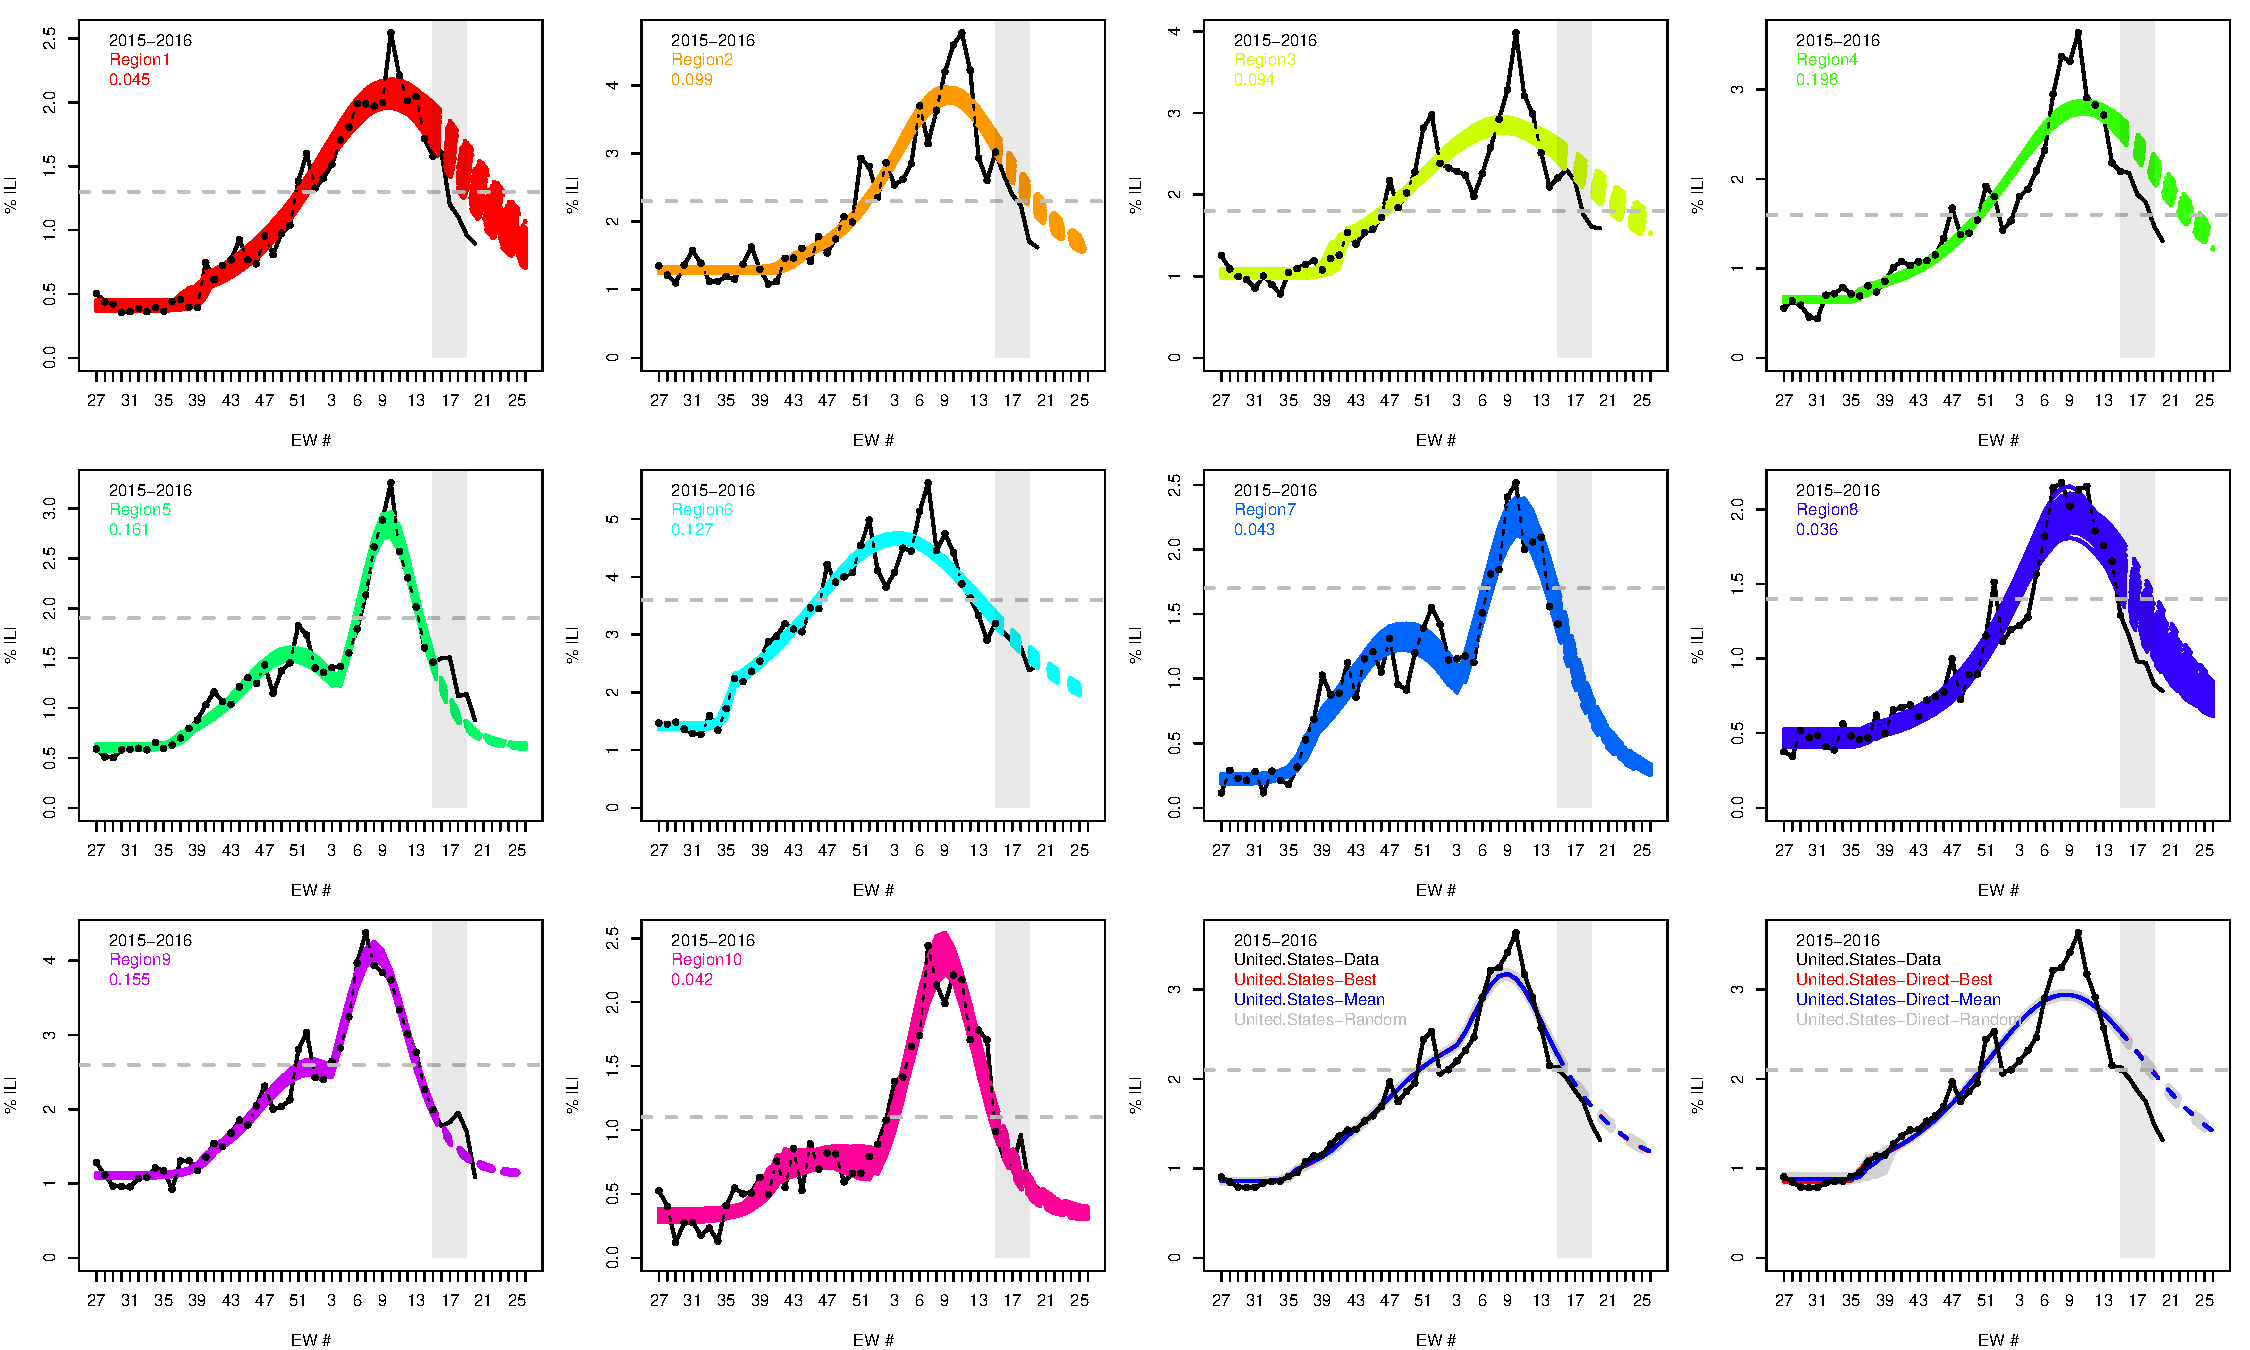
\includegraphics[width=\linewidth]{figures/results-cdc-2015-2016-5-41-1.pdf}
  \caption{Sample \pkg{DICE} output as \%ILI as a function of Epidemic Week (EW) using the following parameter values: disease = `flu', year=2015,  model=5, nfit=41, nMCMC=$10^5$. }
  \label{fig:results}
\end{figure}

\begin{figure}[hbtp]
  \centering
  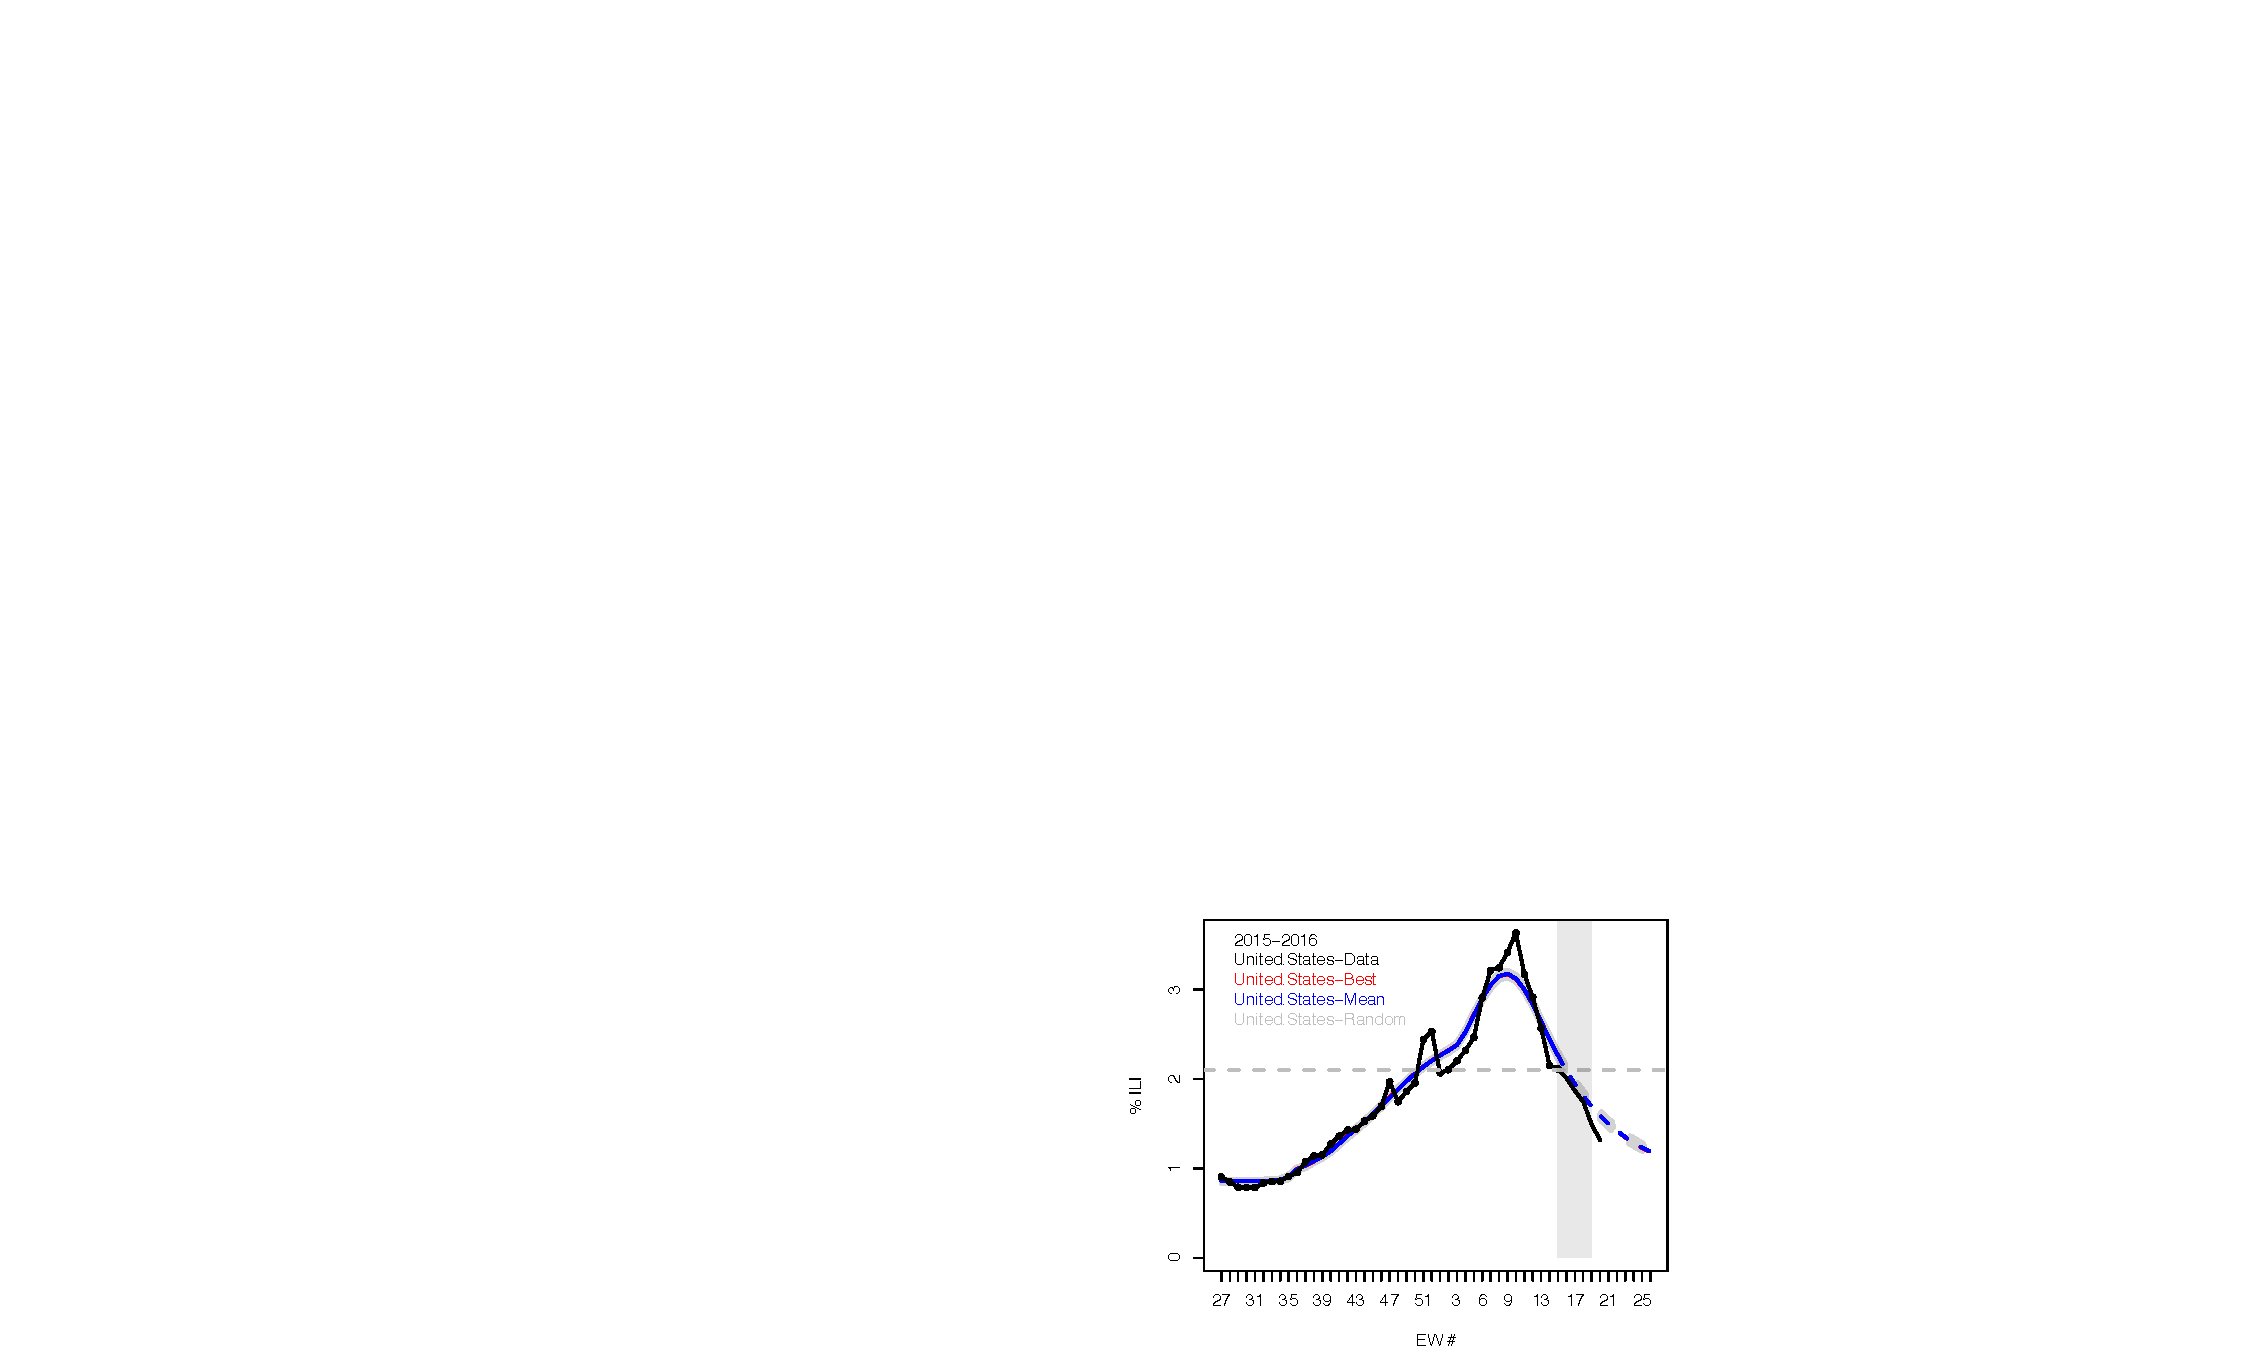
\includegraphics[width=2.75in]{figures/US2015_region_fit.pdf}
  \hspace{0.1in}
  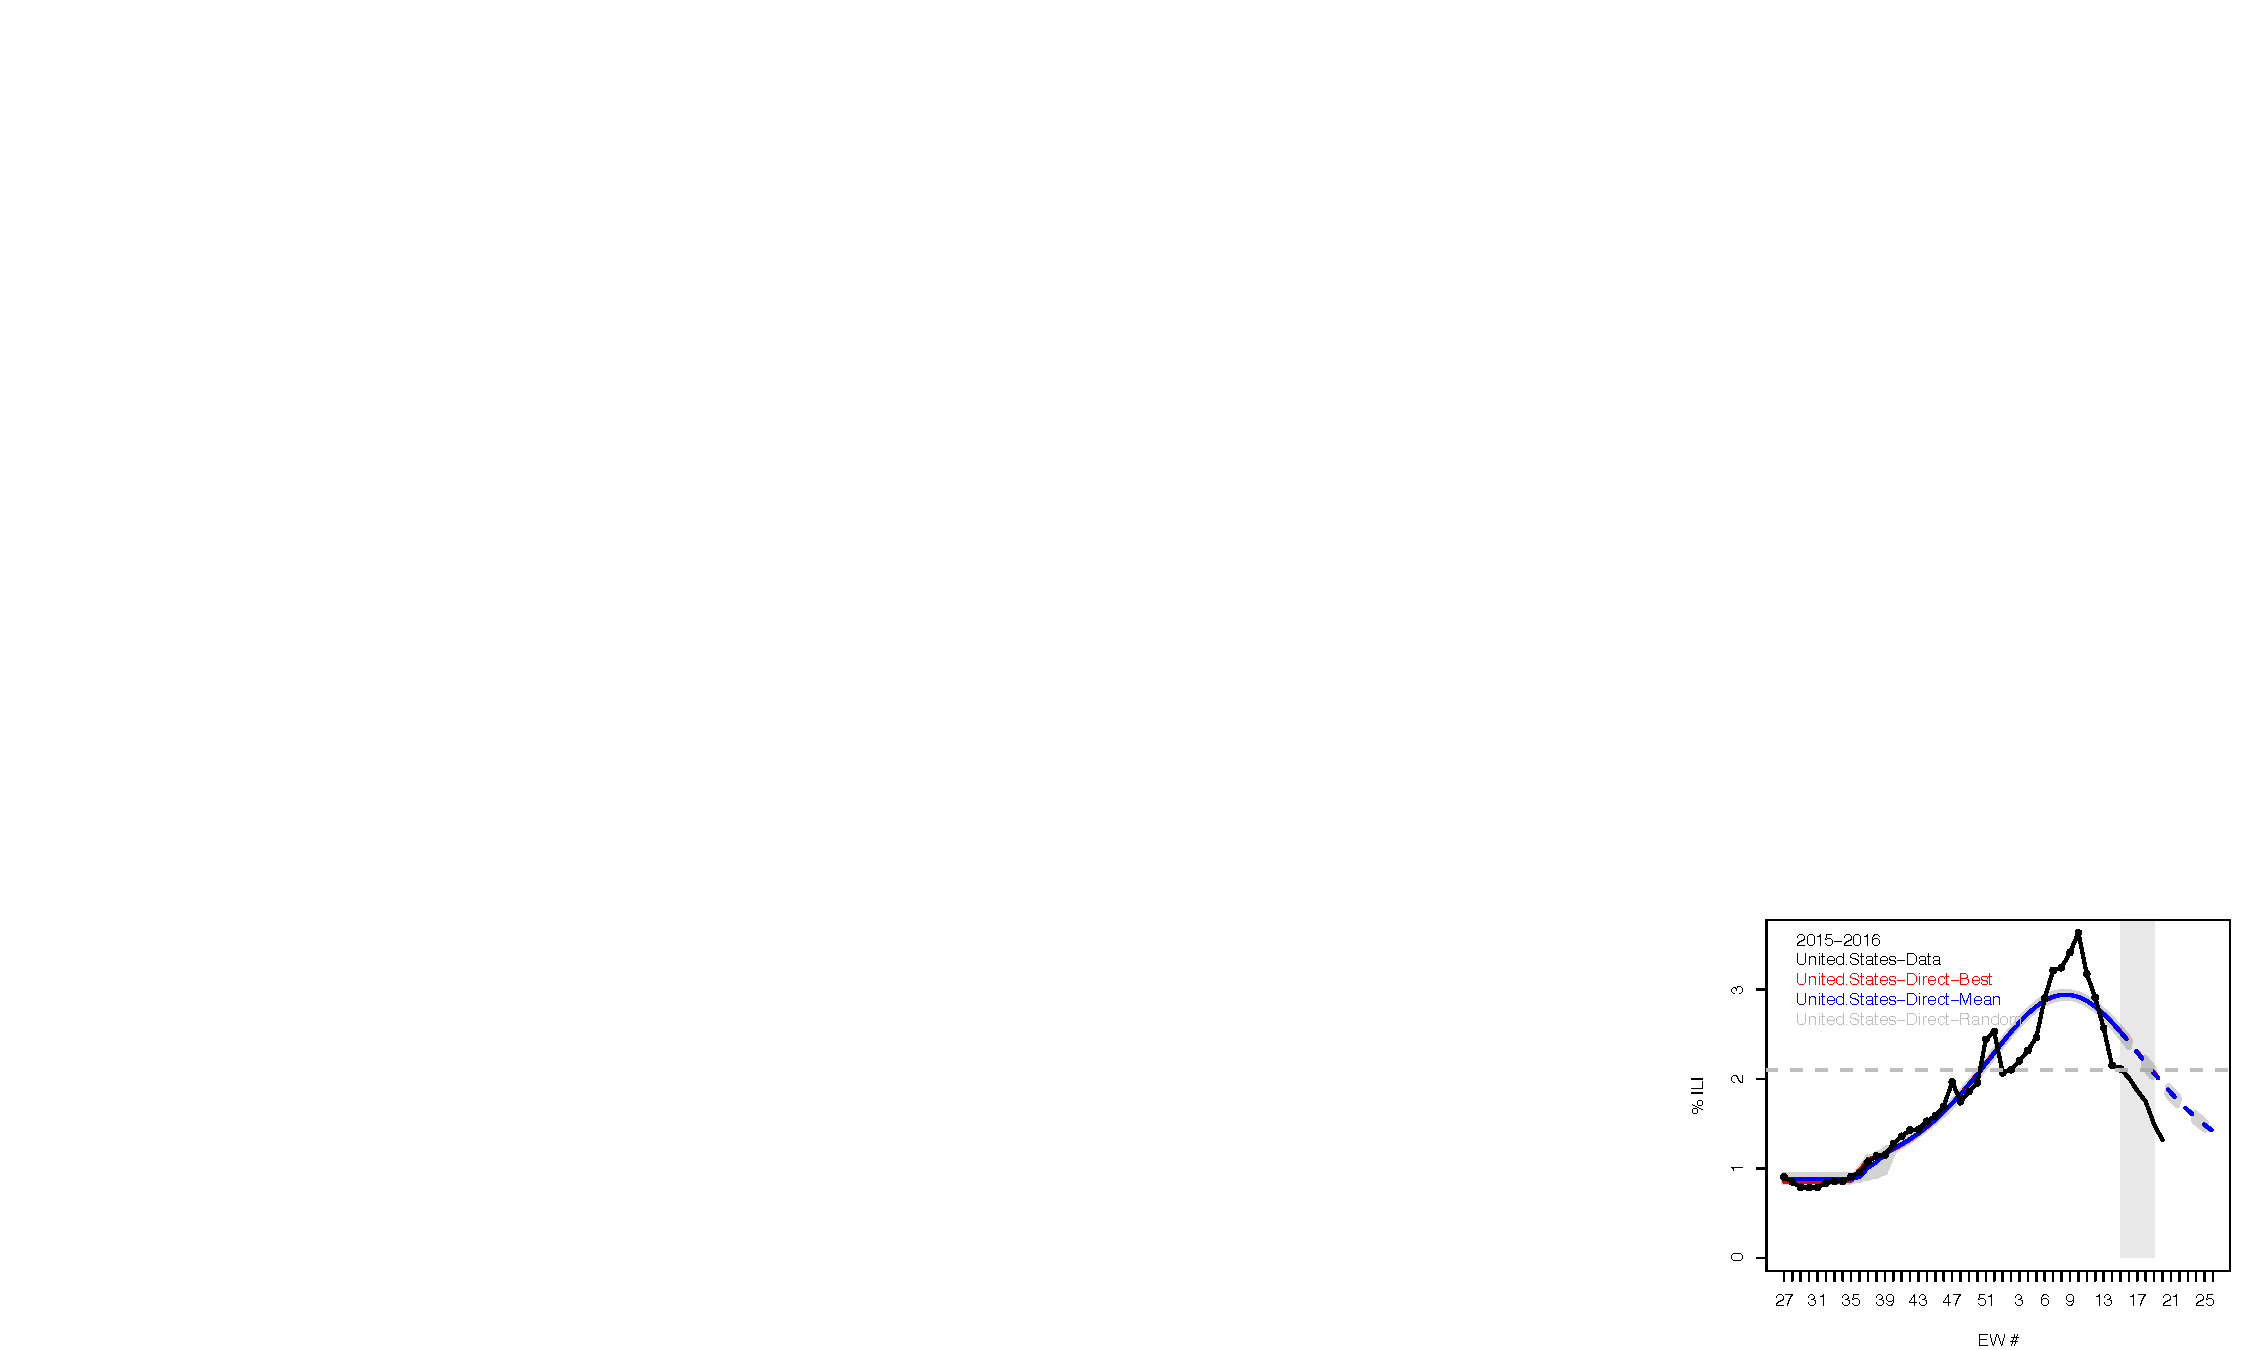
\includegraphics[width=2.75in]{figures/US2015_direct_fit.pdf}
  \caption{Comparing results of a direct fit (right) and region-fit (left) for 2015-2016 national ILI data.}
  \label{fig:nat_results}
\end{figure}


\subsubsection{Peak Week Histogram}
The FileType `hist-week-max' are .pdf files that show the likelihood distribution of peak weeks at both the model and fit level.  The images in figure \ref{fig:peak_hist} come from the file named ``hist-week-max-cdc-United.States-uncpl-2015-2016-5-41-1.pdf".  In these histograms the ILI incidence peaks have been binned by epidemic week number.  The data has a single peak value and is therefore represented by a single blue bar.  The MCMC fitting procedure results in a distribution that is depicted by green bars.  Overlap of data and fit bars is appears as magenta.
\begin{figure}[htbp]
  \centering
  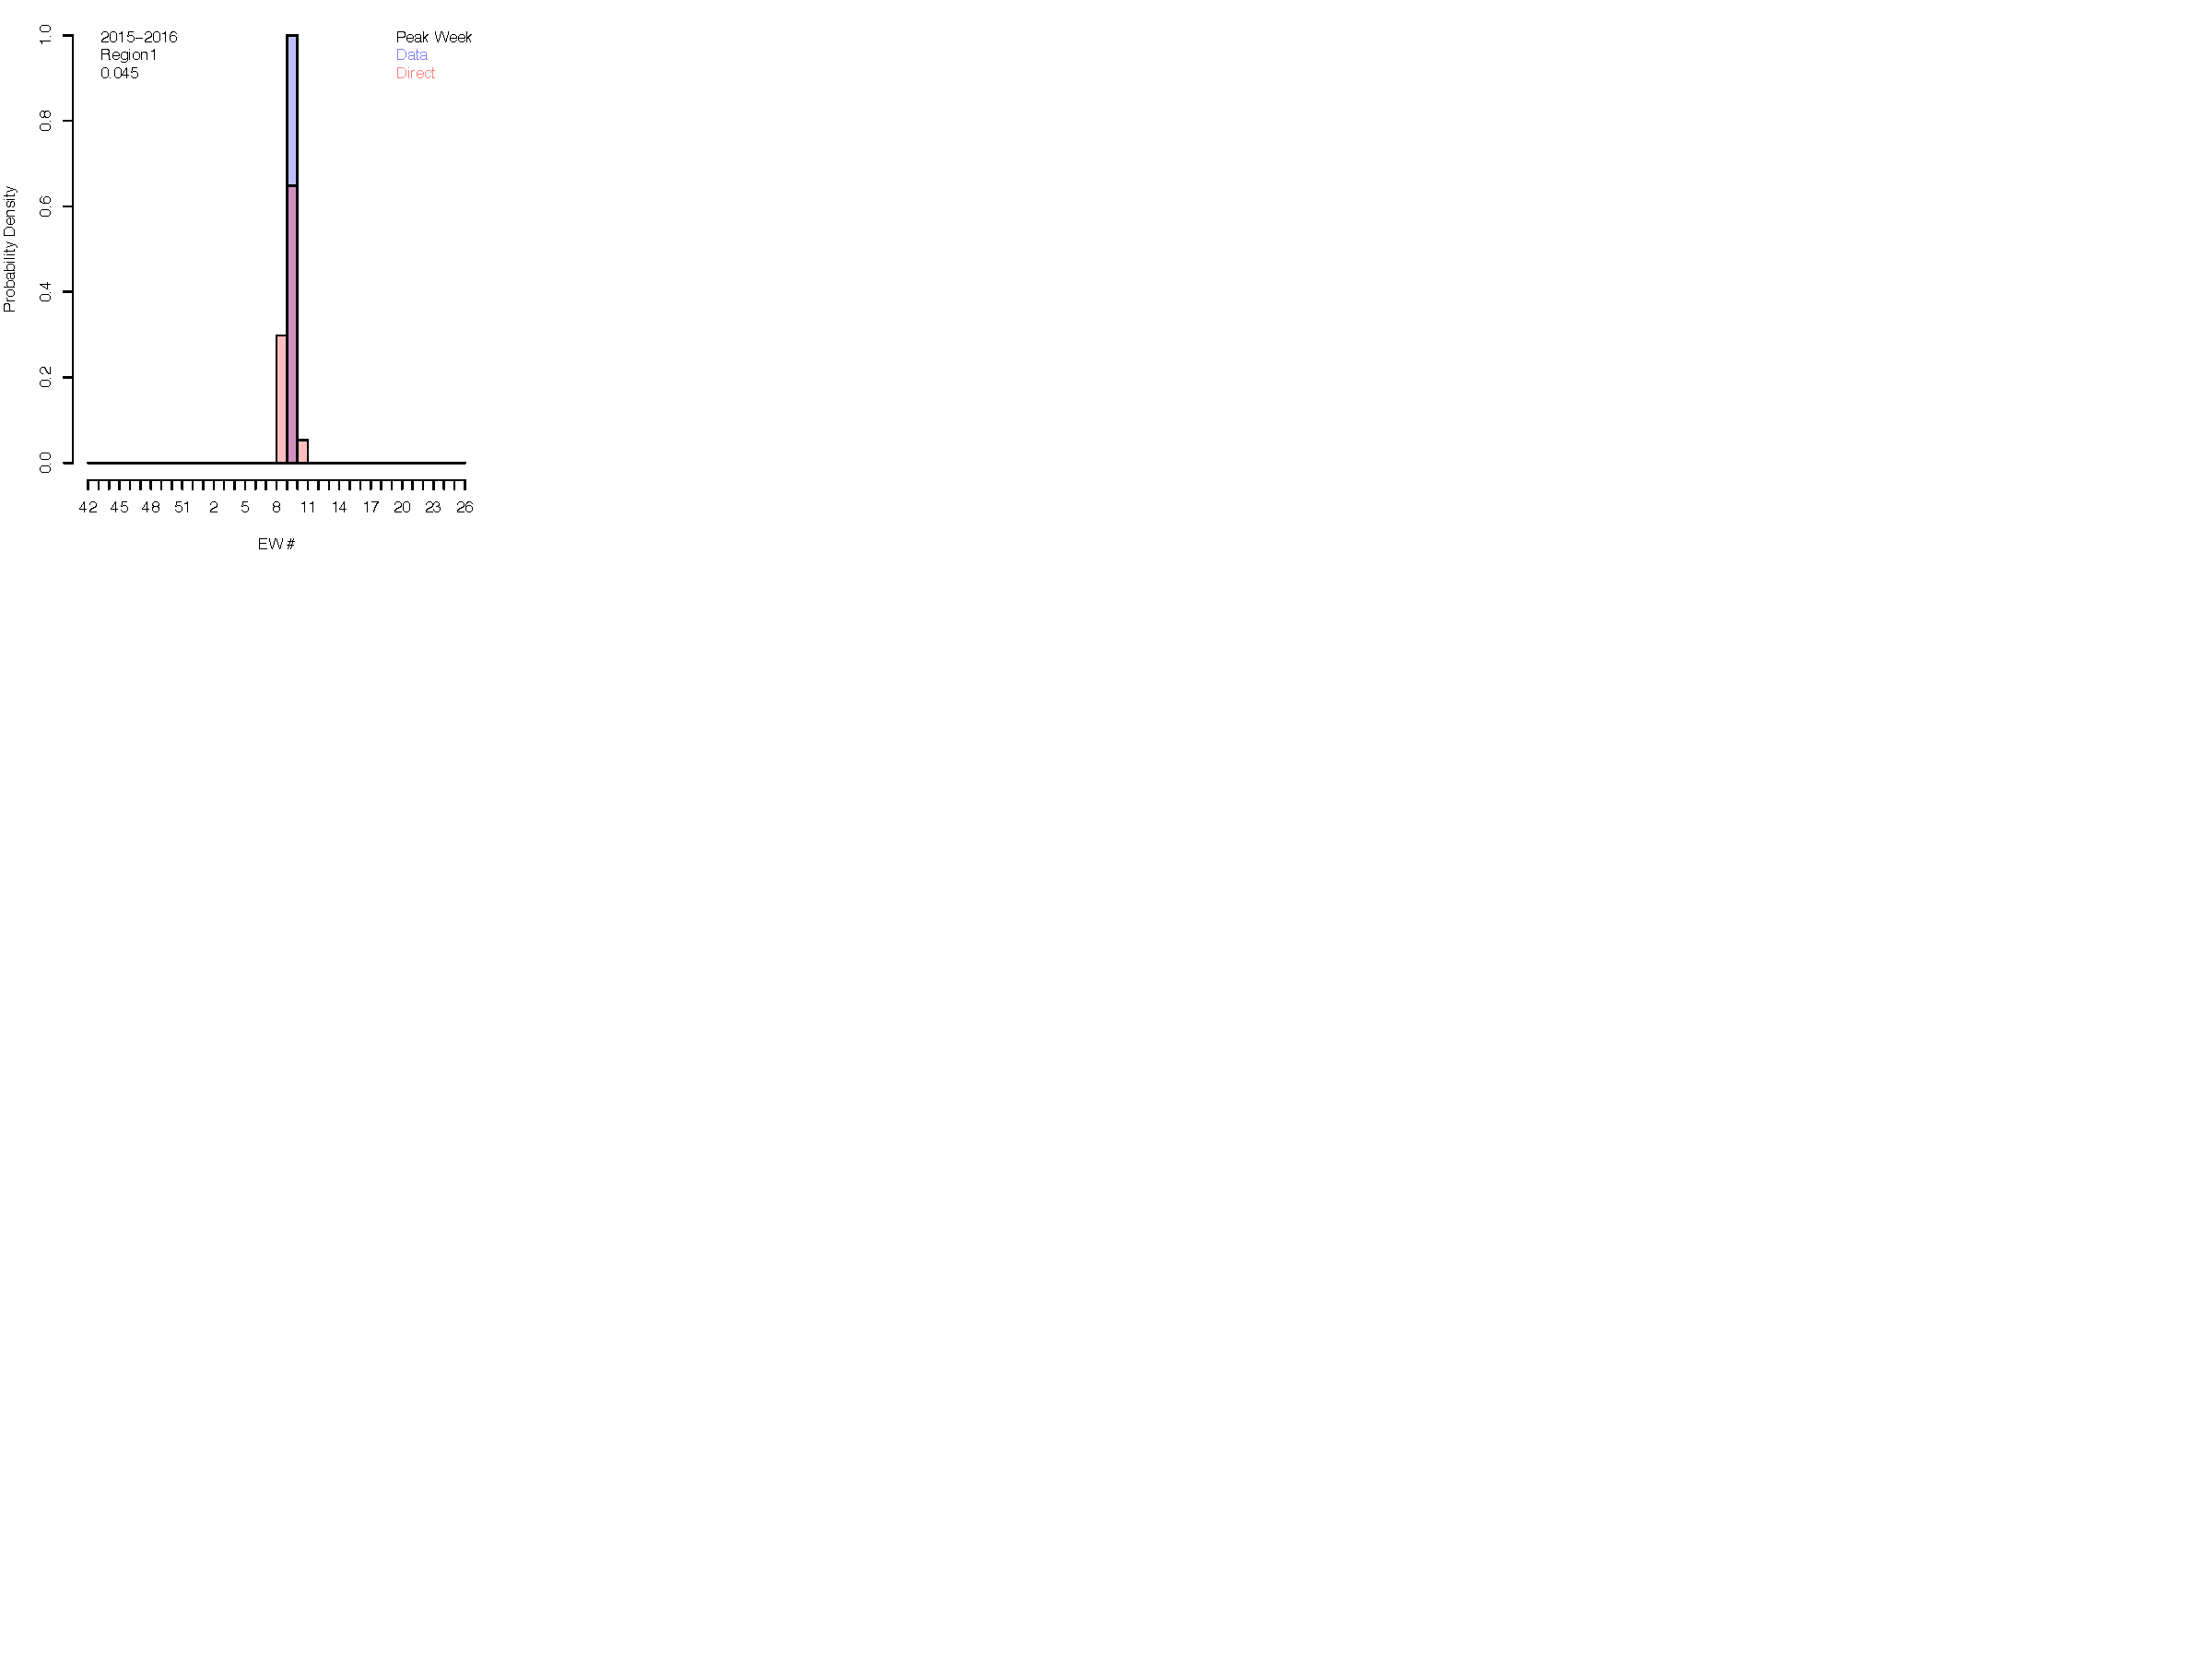
\includegraphics[height=2.75in,keepaspectratio]{figures/Reg1_2015_hist_peak.pdf}
  \hspace{0.4in}
  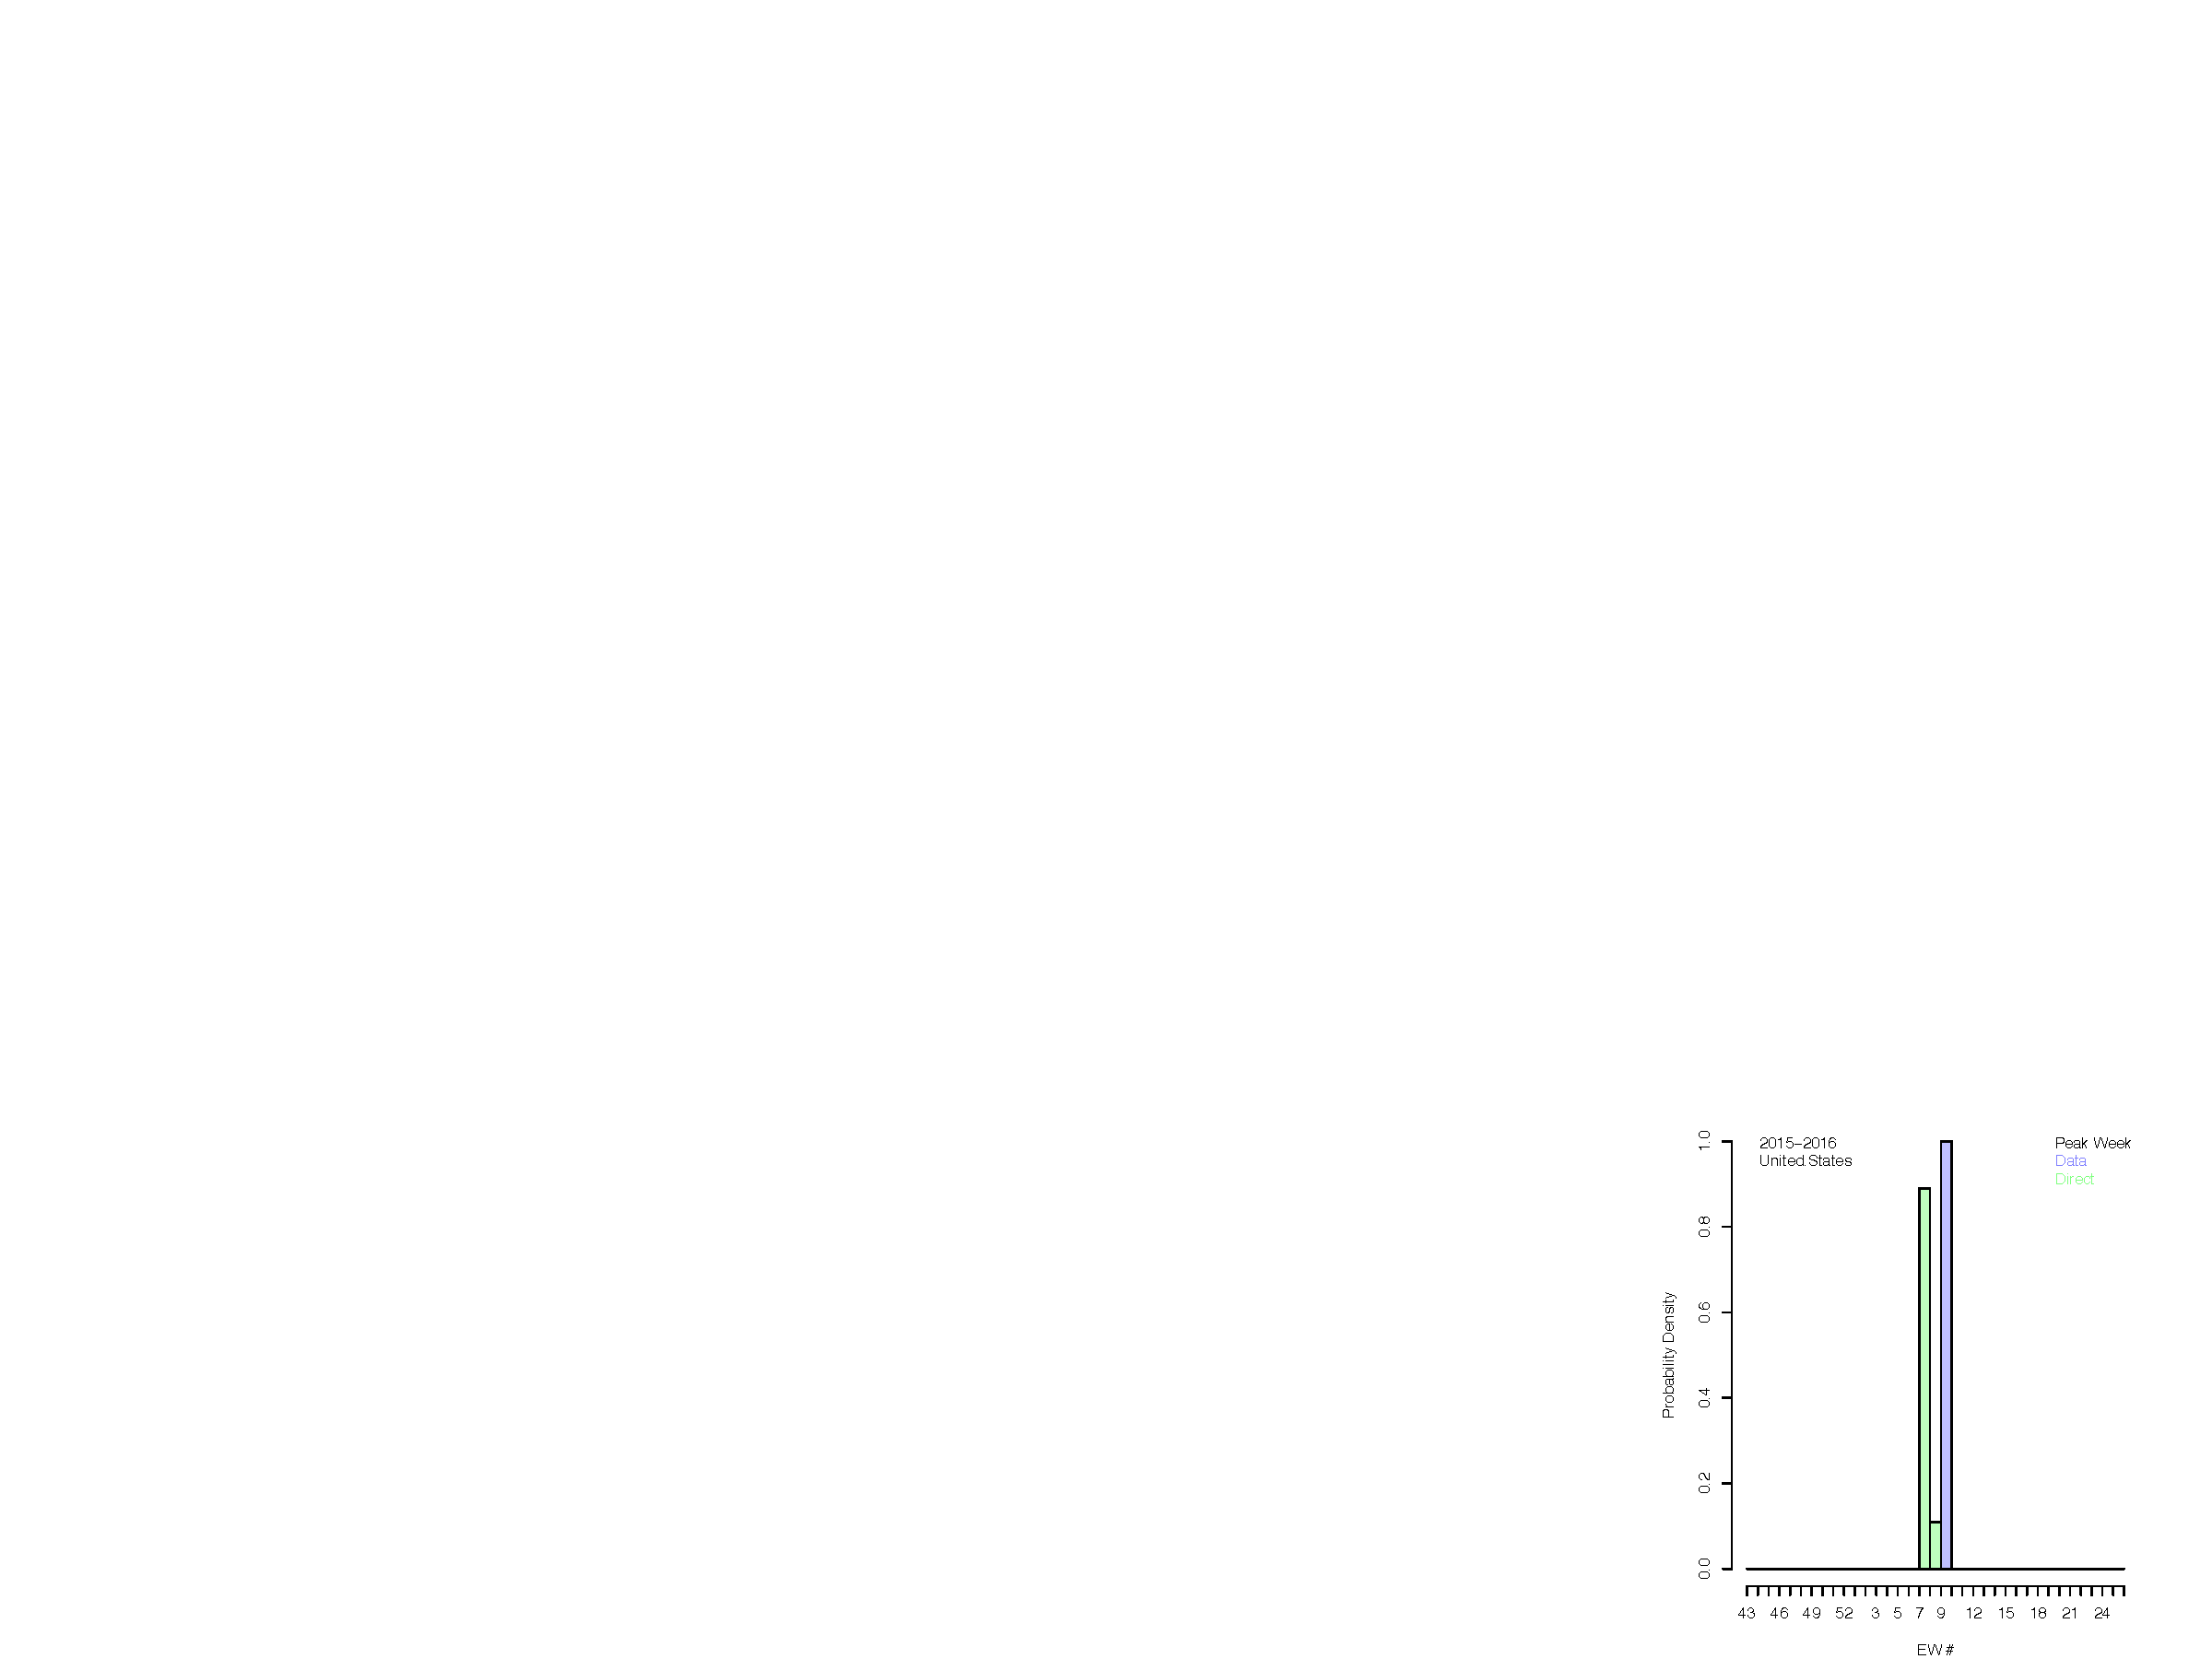
\includegraphics[height=2.7in,keepaspectratio]{figures/USdirect_2015_hist_peak.pdf}
  \caption{Sample histograms for the ILI peak-week distribution. For Region 1 (left) the blue bar depicts the peak data week and the green bars show the distribution of peak weeks found by MCMC fit.  The overlap between the fit and data histograms appears as magenta.  The national direct-fit (right) is colored similarly.}
  \label{fig:peak_hist}
\end{figure}

\subsubsection{Forecast Weeks Histogram}
The FileType `hist-prfl' are .pdf files that show the likelihood distribution for each of the forecast weeks at both the model and fit levels.  Figure \ref{fig:hist_fore} shows the forecast epidemic weeks 15-18 for HHS Region 1.  These images were extracted from the file ``hist-prfl-cdc-United.States-uncpl-2015-2016-5-41-1.pdf".  As was done in the CDC flu challenge, \%ILI is separated into 0.5\%-sized bins.  These plots allow one to compare what \pkg{DICE} predicts for a forecast week to the actual observed \%ILI for that week.  Similar to the previous histogram, the data bar is blue and the forecast bars are green.  Again, where there is overlap between the data bar and forecast distribution, the bar has been colored magenta.  Note that the histograms have been normalized such that the area under the distribution is equal to 1.  Thus the bin size of 0.5 dictates a max bar height of 2.
\begin{figure}[htbp]
  \centering
  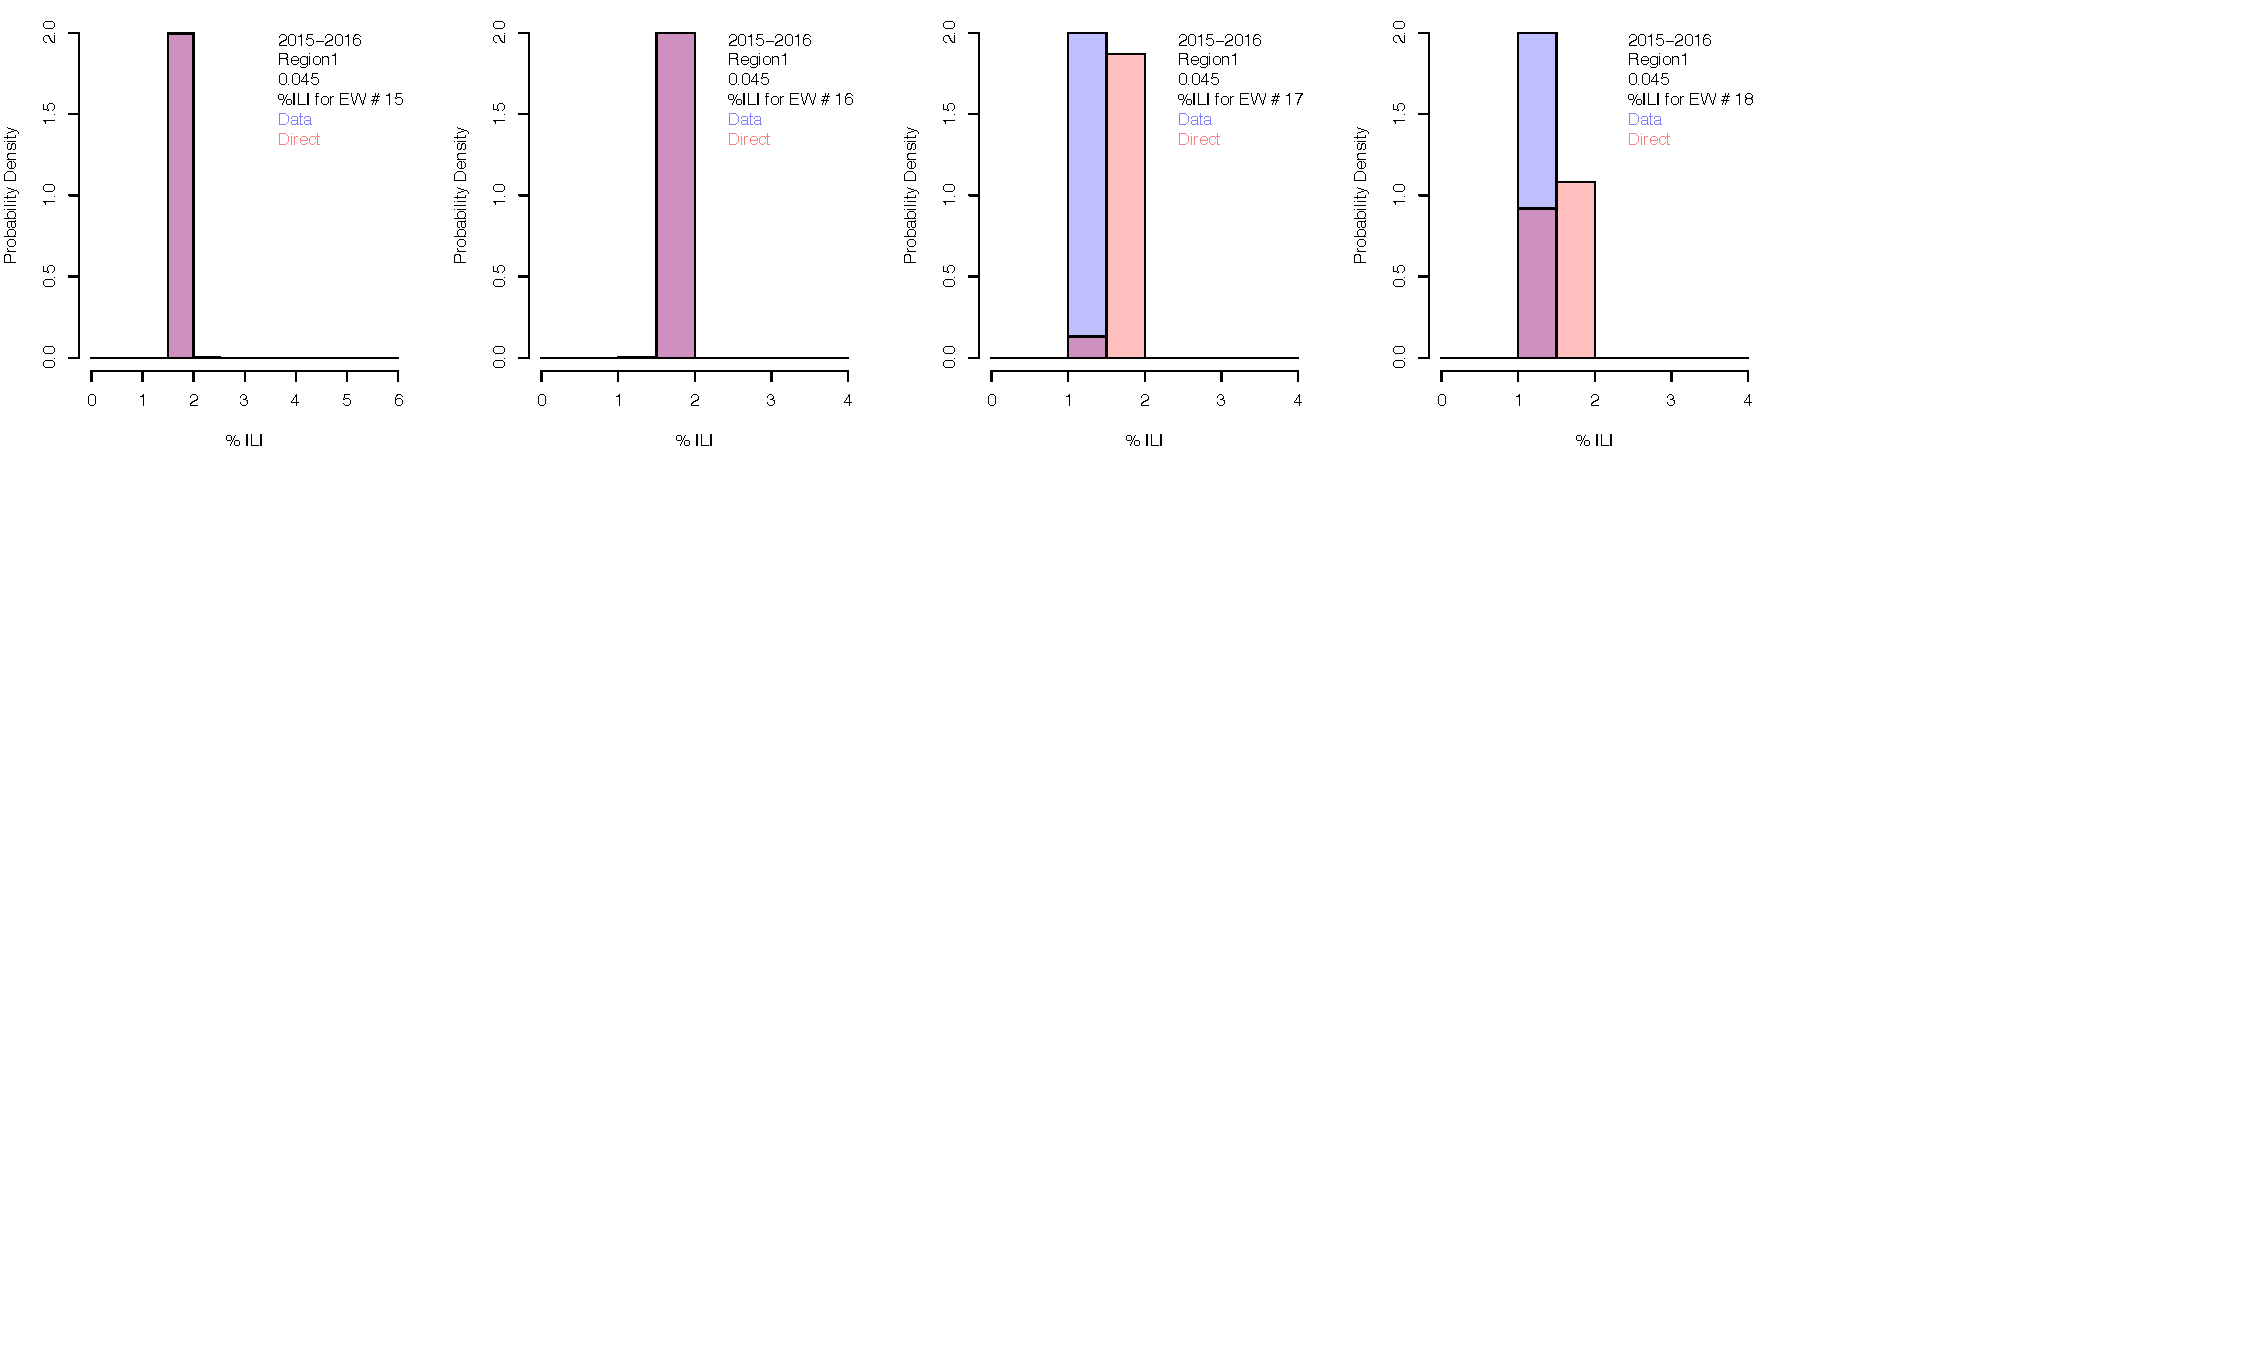
\includegraphics[width=\linewidth]{figures/Reg1_2015_hist_forcast.pdf}
  \caption{Sample histogram for the ILI forecast weeks of a Region 1 fit. Each plot represents the distribution of \%ILI for a single forecast week.  As with the previous figures, this results from the parameters: year=2015, disease = `flu', model=5, nfit=41, nMCMC=$10^5$.}
  \label{fig:hist_fore}
\end{figure}

\subsection{Incidence Profiles Fit-non ILI Example}
The incidence profile fits/forecasts for diseases other than the flu show the same results as in the case of ILI data described in section \ref{sec:resultsGraphics}. As an example we show in figure \ref{fig:br_dengue} the profiles of an uncoupled fit to Dengue data from Brazil for the 2009-2010 season using the five regions of Brazil ($fit\_level = 3$ and $mod\_level = 2$) and an S-E-I-R model ($epi\_model = 2$ or `SEIR').
The Dengue data is monthly number of cases and it is shown with the black line/circles in each panel.  The top row and middle left and  middle center panels, show the fits to each of the five regions. The aggregate fit to the nation level data (middle right panel) is the sum of the region level fits and the bottom left panel shows the results of a direct fit to the nation level data.  The grey line in each panel is a historic NULL model given by the average monthly number of Dengue cases in each region/nation.
\begin{figure}[htbp]
  \centering
  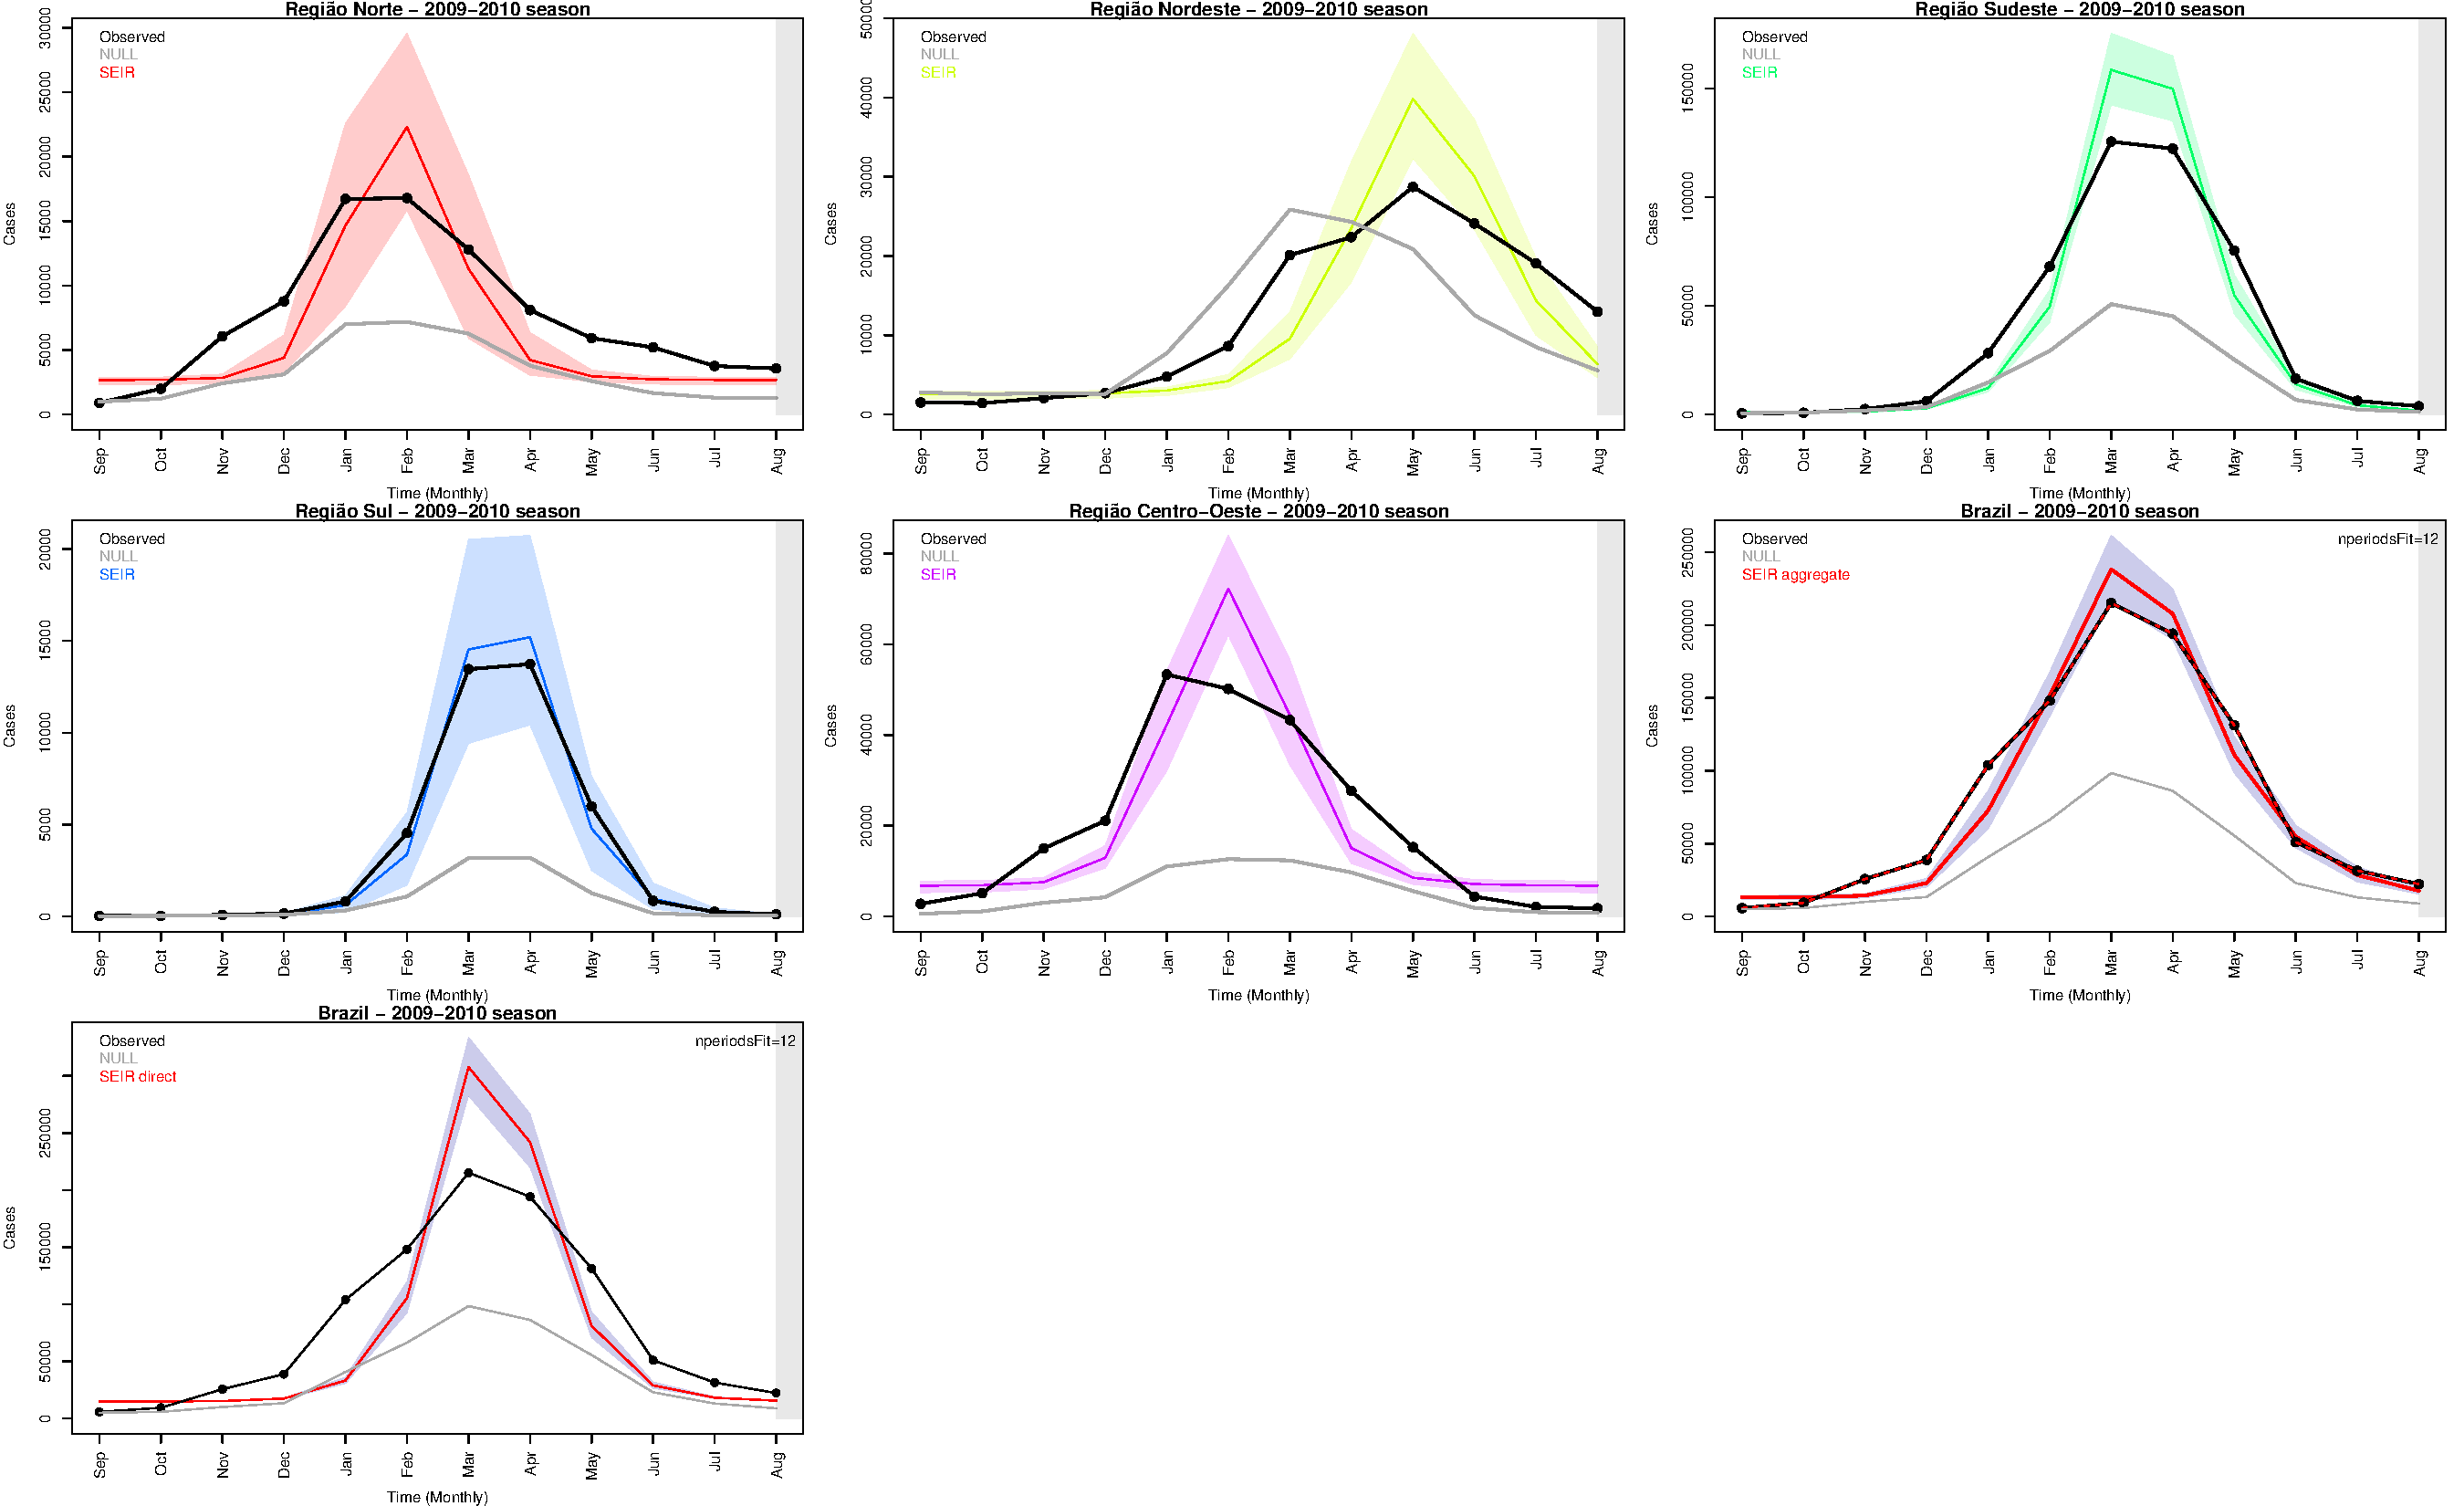
\includegraphics[width=\linewidth]{figures/BR_2009-2010_SEIR.pdf}
  \caption{Example of fits to monthly Dengue data from Brazil using region and nation level data. These results are from the parameters: year=2010, disease=`dengue', RegState = 'BR', mod$\_$level = 2, fit$\_$level = 3, isingle = 1, epi$\_$model = 'SEIR', model=4, nfit=12, nMCMC = 1e6}
  \label{fig:br_dengue}
\end{figure}

\subsection{Data Files}
Here we briefly summarize the contents of the data files generated by a \textit{runDICE}() simulation.  The five types of data files produced by \pkg{DICE} are described below.

\subsubsection{Input Data and Parameters}
FileType `input' records all of the model and data inputs to the fitting procedure.  In this example the filename is ``input-cdc-sir-United.States-uncpl-2015-2016-4-41-1.RData".  This file contains two R objects, the first is called `input' and details all model parameter values (generated from user inputs).  The second object `mydata' contains all data generated by \pkg{DICE} for the simulation.

\subsubsection{MCMC Chain}
The raw results from the MCMC fitting procedure are contained in the `mcmc' FileType.  For this example the filename is ``mcmc-cdc-sir-United.States-uncpl-2015-2016-4-41-1.RData".  The R object `results.list' is a list of MCMC chains.  There is one list entry for each population that was fit during the MCMC procedure.  Each list entry is a representative sampling of the MCMC history.  This takes a matrix form with each row corresponding to a sample and each column an optimized parameter.  This file is the primary output of a simulation, and it is also useful for the purpose of restarting the chain.

\subsubsection{ILI Profiles}
The `profiles' FileType is and .RData that stores a representative sample of ILI profiles generated by the MCMC chain.  For this example it is named ``profiles-cdc-sir-United.States-uncpl-2015-2016-4-41-1.RData".  This file contains all information needed to plot the direct and aggregate profiles on the model-level.

\subsubsection{Forecast Weeks LLK}
When the forecast weeks overlap with observed data, the Log-Likelihood (LLK) is calculated and stored in FileType `llk'.  For the example simulation in this section the filename is: ``ili-cdc-sir-United.States-uncpl-2015-2016-4-41-1.csv".  This information is useful for quantitatively comparing forecasts of the aggregated and direct fits.

\subsection{Season Targets}
The file ``stats-cdc-sir-United.States-uncpl-2015-2016-4-41-1.csv" contains the observed and predicted (best, mean and standard deviation) values for: onset week, peak week and peak intensity for the model level and fit level regions.

\subsubsection{Gaussian Fit}
The file ``gaussian-fit-cdc-sir-United.States-uncpl-2015-2016-4-41-1.csv" contains a mean and variance for each optimized parameter.  This procedure fits a single variable Gaussian to the parameters one-by-one.  While this approximation of mean and variance is often quite useful, it should be noted that the distribution returned by the MCMC procedure is a function of many parameters.  The parameters are interdependent, and thus a single variable Gaussian may be a poor approximation of the large-dimension distribution. Nevertheless, these fits are useful if the user wishes to use a prior distribution in the MCMC procedure.  This has been explored in the context of the CDC challenge for the 2015-2016 flu season.

\subsection{Output Files For Statistical Runs}
In the case of a statistical run the number of output files is significantly smaller and the directory and file name convention are simpler. As an example we use the 2010 Dengue data for Brazil which we model with a specific SARIMA model and precipitation as a covariate with a lag time of one month:

\begin{verbatim}
> arima_model = list(p = 1, d = 0, q = 0, P = 3, D = 1, Q = 0)
> covar = 'precip'
> covar_lag = 1
\end{verbatim}

\pkg{DICE} is called using:

\begin{verbatim}
> runDICE(disease = 'dengue', RegState = "BR", year=2010, mod_level=2,
      fit_level=3, nfit=12, method='stat', arima_model = arima_model,
      covar= 'precip', covar_lag = 1)
\end{verbatim}
all the output files appear in a directory called ``Brazil\_2010\_level\_2/" and the filename convention for the output files is:

\begin{verbatim}
  "FileType-sarima-source-Mod_Reg-Year-SarimaModel-covar-lag-nfit.FileFormat"
\end{verbatim}
where \textbf{source} is the name name of the data source, \textbf{Mod\_Reg} is (as before) the name of the model region, \textbf{Year} is the season, \textbf{SarimaModel} is the detail of the sarima Model we chose, \textbf{covar} is the covariate name, \textbf{lag} is the lag time for the covariate and \textbf{nfit} is the number of data points fitted. The statistical run produces two graphic files. The first graphic file contains the results.  It is named in this case: ``results-sarima-bra\_mh-Brazil-2009-2010-100-310-precip-lag-1-12.pdf" and shown in figure \ref{fig:sarima_results}
\begin{figure}[htbp]
  \centering
  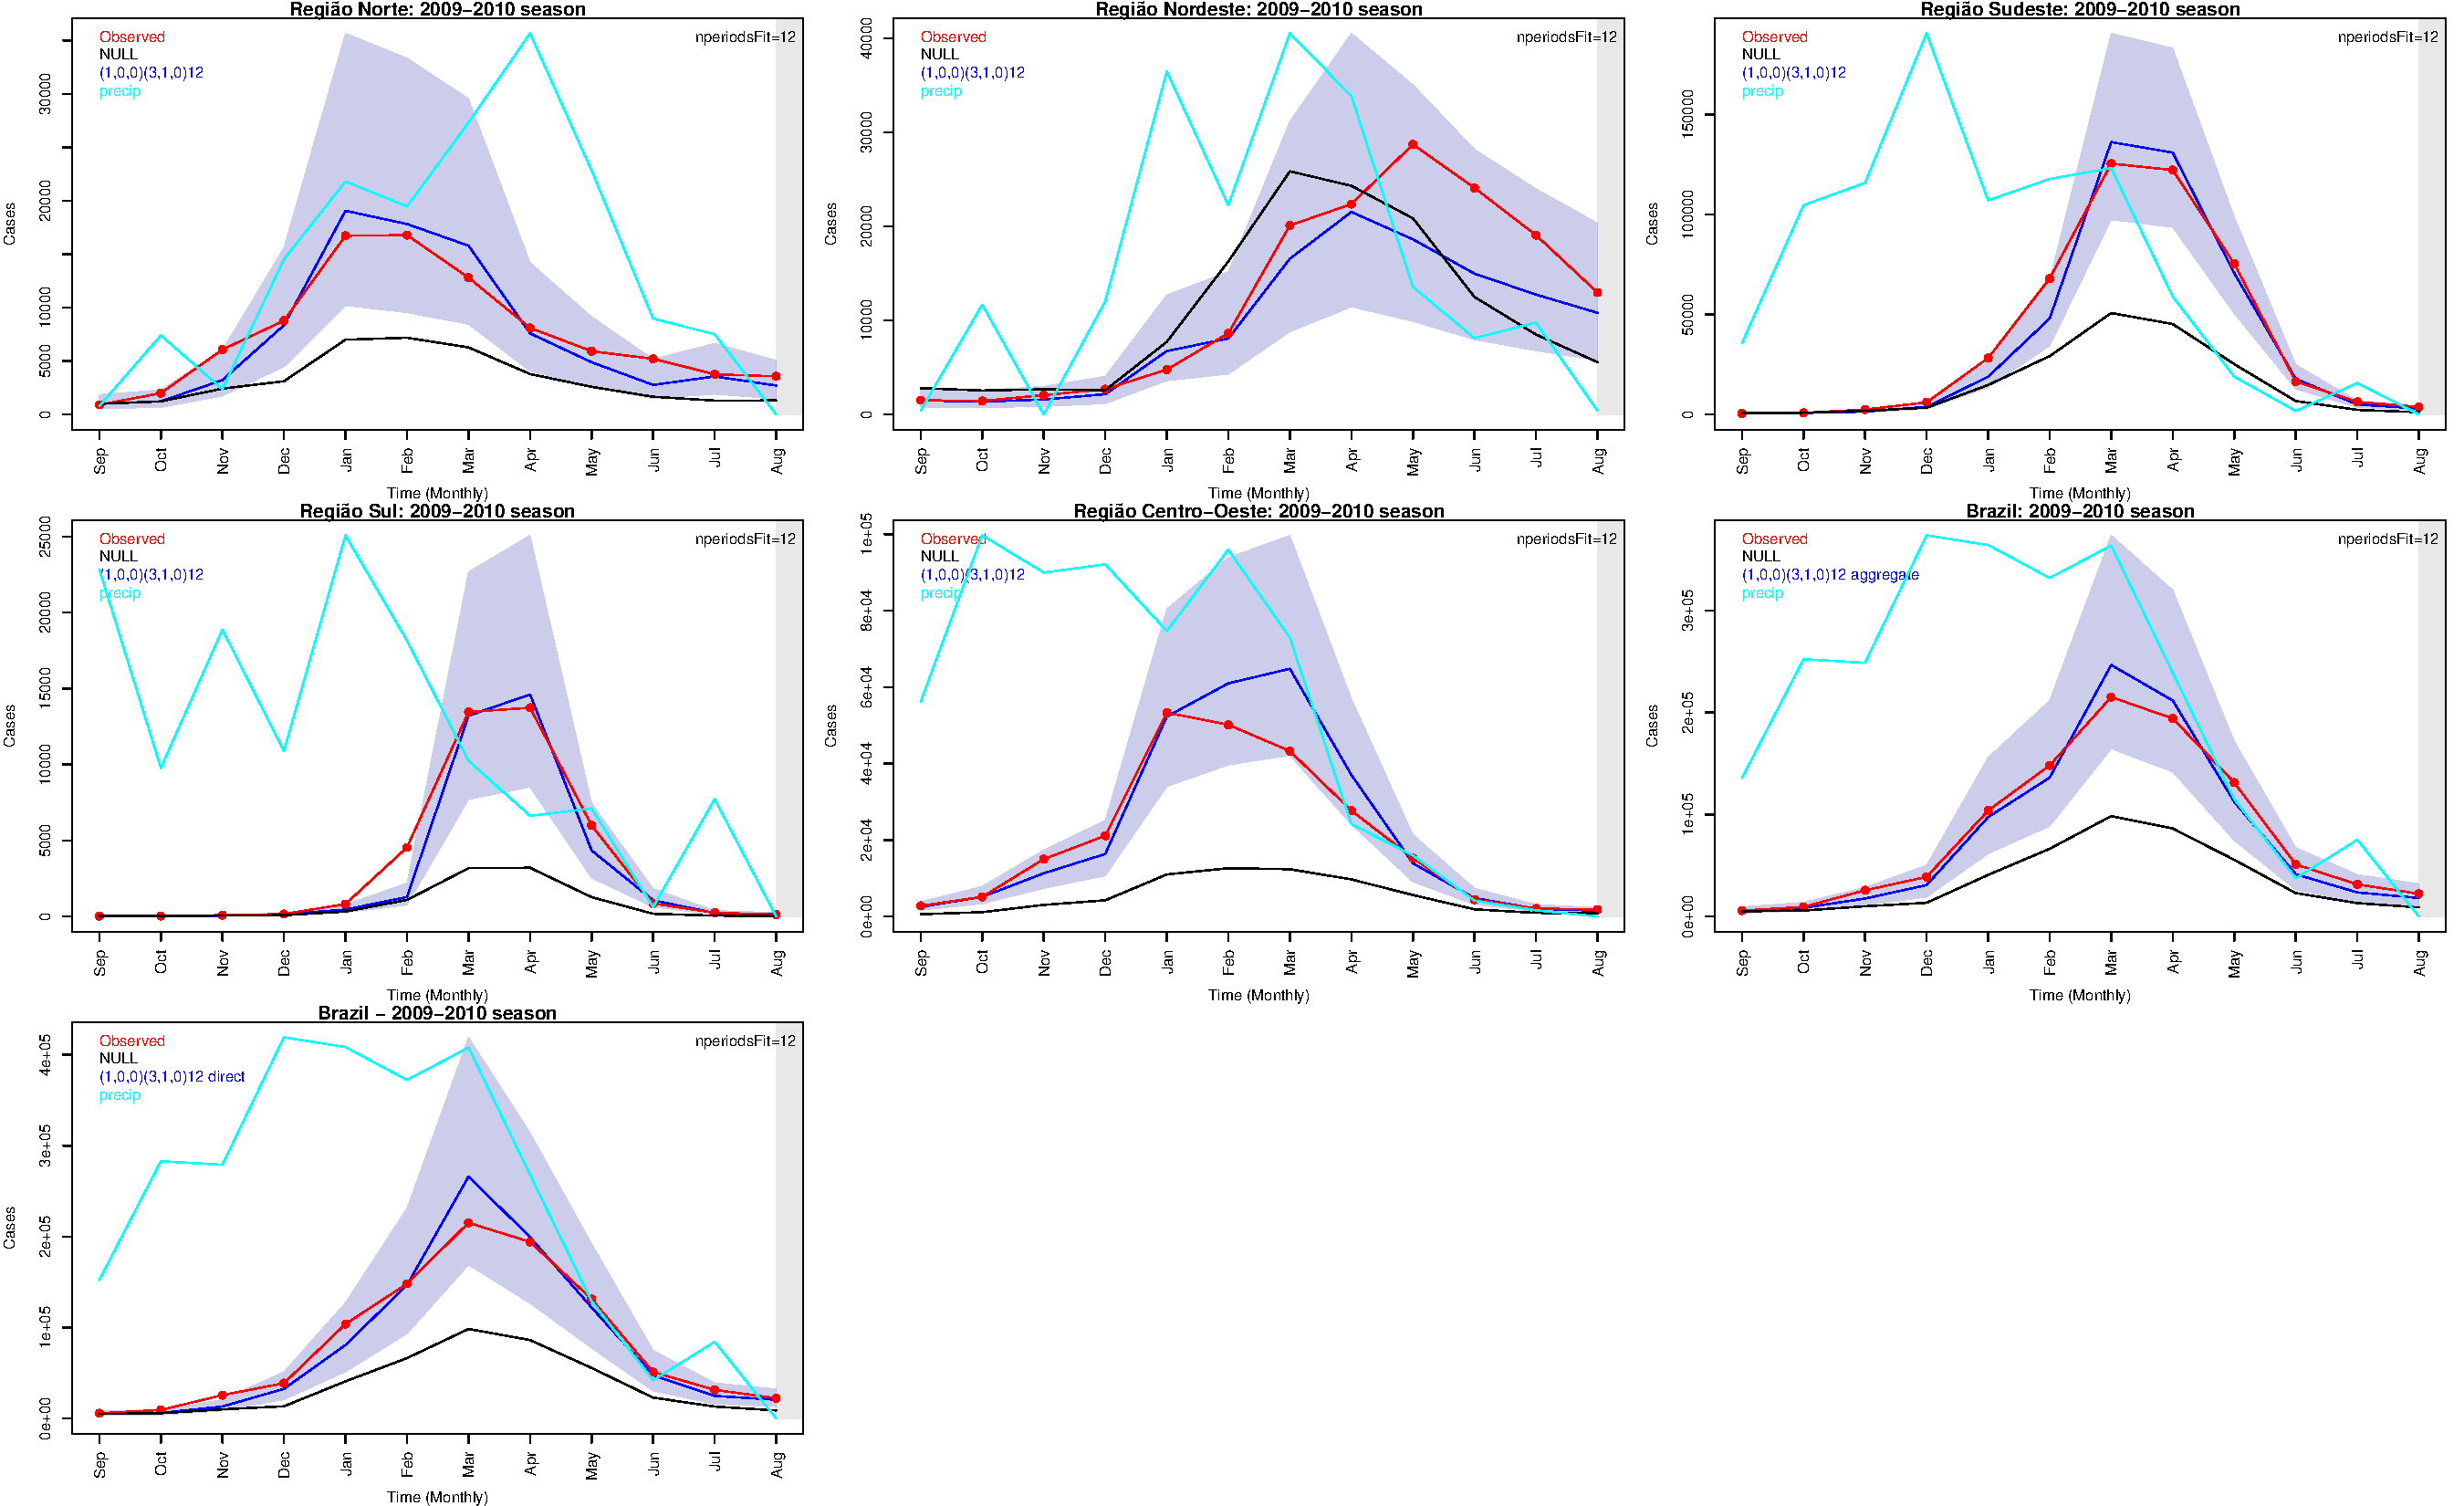
\includegraphics[height=2.75in,keepaspectratio]{figures/sarima_results.pdf}
  \hspace{0.4in}
  \caption{Sample of SARIMA fits to the region and national level Dengue Data for Brazil. The first five panels (top row and left/middle panels in the second row) show the fits to the five regions followed by the aggregate fit to the National curve (right panel in second row). The last panel (bottom row) is the result of the direct SARIMA fit to the national incidence. The red line in each panel is the data, blue line is the fit and the shaded region denotes the standard deviation.  The black line in each panel is the historic average which we call the ``NULL'' model. The legend in each panel denotes the SARIMA model and the cyan line is the covariate (precipitation in this example).}
  \label{fig:sarima_results}
\end{figure}

The aggregate fits are obtained by simply adding the fits to the five regions.
The second graphic file compares the fit/forecast to the observation by depicting the error. It is called in this case:
``error-sarima-bra\_mh-Brazil-2009-2010-100-310-precip-lag-1-12.pdf'' and shown in figure \ref{fig:sarima_error}:


\begin{figure}[htbp]
  \centering
  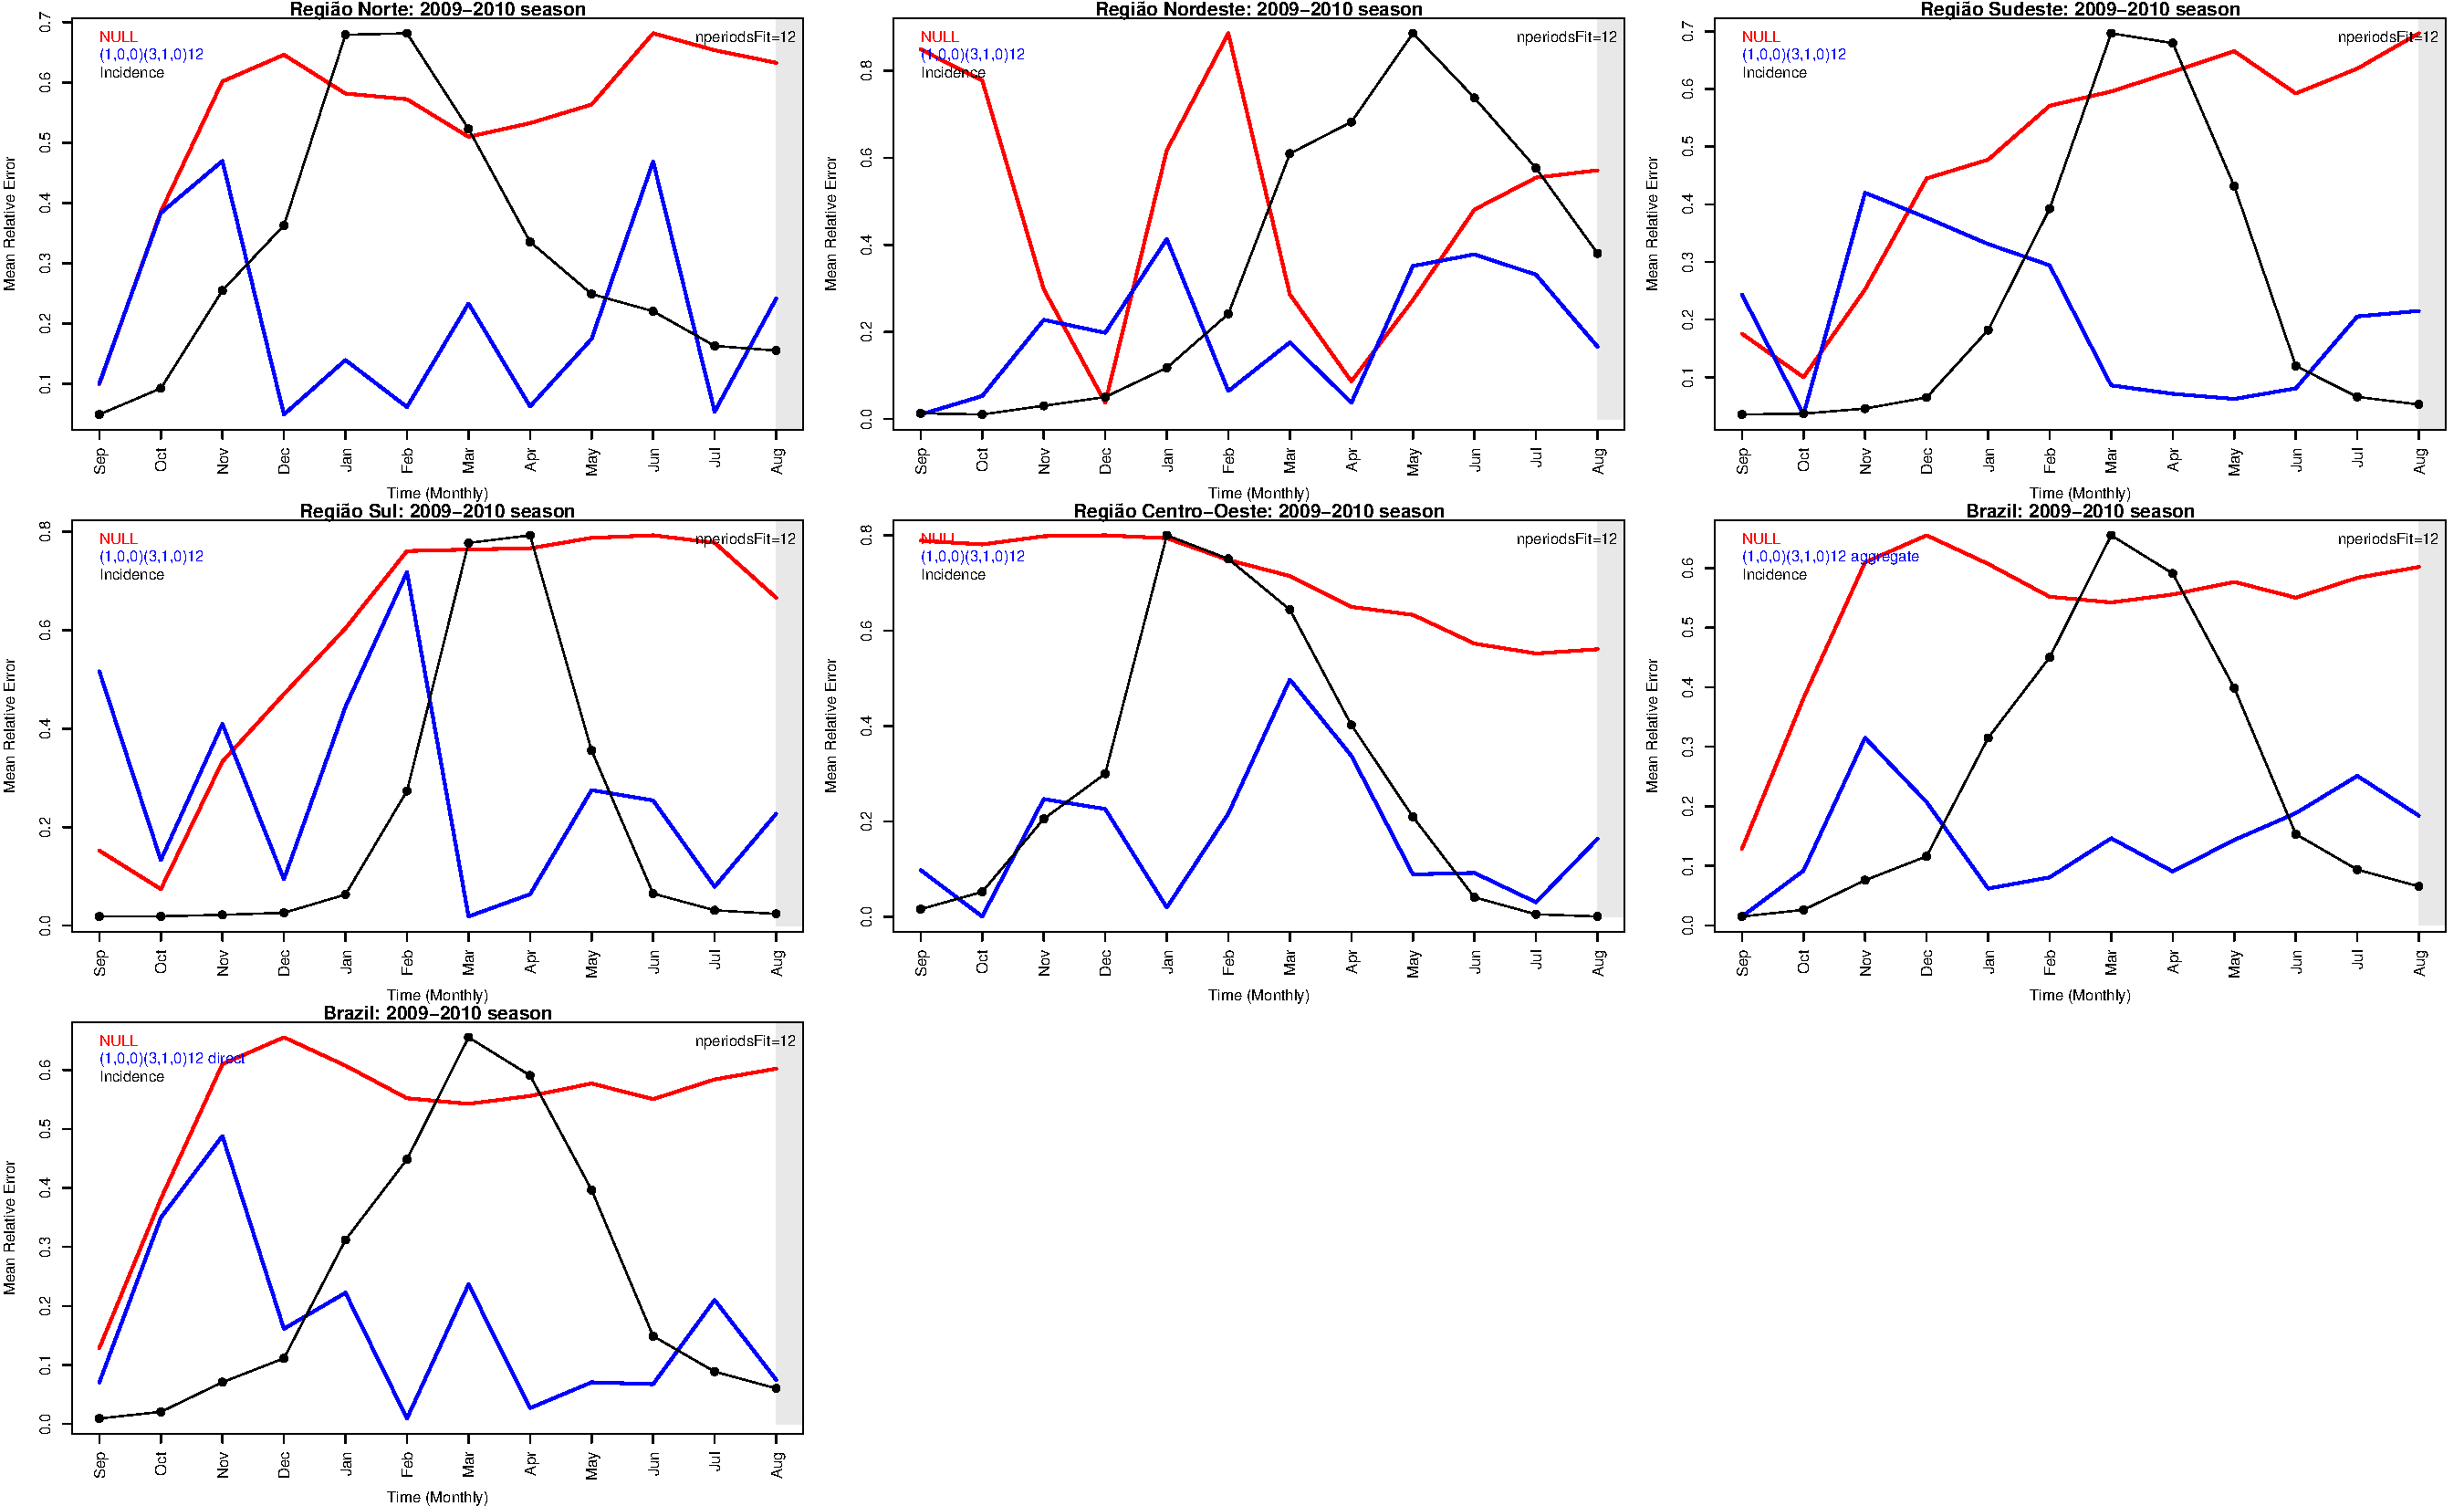
\includegraphics[height=2.75in,keepaspectratio]{figures/sarima_error.pdf}
  \hspace{0.4in}
  \caption{The error of the SARIMA fits shown in the previous figure. The black line/dots are the observed incidence and the blue line is the mean relative error (MRE) of the SARIMA fit.  In red we show the MRE error of the historic NULL model. The panels are ordered as before: five regions followed by nation aggregate and nation direct (bottom panel). }
  \label{fig:sarima_error}
\end{figure}

The statistical runs produce a single binary file named in this example: ``sarima-bra\_mh-Brazil-2009-2010-100-310-precip-lag-1-12.RData".  This file contains all the data used for this run, the details of the SARIMA model and tables with the results of the fit/forecast.   This file can be loaded to produce additional plots.

Before concluding this section we note that if the user does not define a SARIMA model, and lets \pkg{DICE} select the best model for each region and the nation, the output file names replace the ``SarimaModel-covar-lag" part with ``auto-arima". In this case, the legend of each panel in the plot files will denote the specifics of the SARIMA model chosen by \pkg{DICE} for each region/nation.

\section{DICE Key Words}
\label{sec:keyWords}
The following is a list of all key words recognized by the \pkg{DICE} package:
\begin{itemize}
\item \bold{db$\_$opts} A list of database options.  DICE$\_$db Determines which SQL database the data is retrieved from.  'PredSci' is the default SQL database, `BSVE' is in development.  Additional flags are for outside sources of data (currently only the CDC Influenza-Like$\_$Illness (ILI) is supported: CDC$\_$server=TRUE).
\item \bold{disease} String - disease name. Options for modeling are: flu, dengue, yellow$\_$fever, ebola, zika, cholera, chik, plague. To graphically explore the data see: \url{predsci.com/id_data/}. A full list of diseases in the DICE database can be found from an R-prompt by:
\begin{verbatim}
    > library(DICE)
    > myDB = OpenCon()
    > data_sources = dbReadTable(con=myDB, name="data_sources")
    > dbDisconnect(myDB)
    > unique(data_sources$disease)
\end{verbatim}
\item \bold{data$\_$source} - Describes the data source for the incidence data. Default is `cdc' (for \code{disease = `flu'}). It can be selected by source$\_$key (integer) or source abbreviation (string). Most disease/location combinations have only one data source.  In this case, it may be easier to set data\_source=NULL.  However, when multiple data sources exist, setting data\_source=NULL will essentially choose from the available sources at random.  To determine a data source by graphical interface, see: \url{predsci.com/id_data/}.  Looking-up the disease and location will result in a list of data sources that can be entered into DICE.  Alternatively, all country/disease/data\_source combinations are listed in the `Data Sources Table' tab at the same url.  To access the list of sources directly:
\begin{verbatim}
    > library(DICE)
    > myDB = OpenCon()
    > data_sources = dbReadTable(con=myDB, name="data_sources")
    > dbDisconnect(myDB)
    > str(data_sources)
    > data_sources$source_abbv
\end{verbatim}
\item \bold{mod$\_$level} - integer. Spatial level of the model data. The US/CDC covers the following levels: 2-United States, 3-HHS Regions, 4-State.  Level 1 is always continent and level 2 is always country, but the levels of smaller divisions vary by country.
\item \bold{fit$\_$level} - integer. Spatial level of data used for a coupled or uncoupled fit of the model data.  Again, this varies by country and data availability, but fit\_level must always be greater than or equal to mod\_level.
  \item \bold{mod$\_$name} - Named character vector specifying the model-level spatial patch.  If \code{is.null(mod$\_$name)}, the code reverts to using \code{RegState}.  To specify New York state, set \code{mod$\_$name=c(NAME$\_$2="United States", NAME$\_$3="R2", NAME$\_$4="New York")}. Here NAME$\_$X is either the full name or abbreviation of the level-X patch. Replacing `United States' with `US` or `R2' with `Region 2' would result in the same outcome.  Also, vector entries for mod$\_$name should go from NAME$\_$2,....,NAME$\_$n where mod$\_$level=n.
\item \bold{RegState} - name of location to model (default `usa').  This is an older input that has been retained for backwards compatibility.  It is suggested that users use mod\_name instead.  Single element: determines which single region from \code{mod$\_$level} is to be modeled. Depending on the model level, \code{RegState} should adhere to the following format: \code{mod$\_$level = 2} - 3-letter ISO3 code, \code{mod$\_$level=3} - an integer describing the HHS region, \code{mod$\_$level=4} - a 2-letter state code (US). RegState is limited to country-level data and US regions/states.
\item \bold{fit$\_$names} A character vector indicating which fit-regions to use.  If \code{fit\_name='all'}, then DICE uses all child-regions of the model region with level equal to \code{fit\_level}. The other mode for fit\_name is to specifiy a subset of the fit regions to construct an aggregate representation of the model region.  For example if \code{mod\_level=c(NAME\_2="US")}, \code{mod\_level=2}, \code{fit\_level=3}, and \code{fit\_names=c("R1", "R2", "R3")}, DICE will create and model an Atlantic super-region from HHS regions 1, 2, and 3 (as opposed to using all 10 HHS regions).  Similarly, if \code{mod\_level=c(NAME\_2="US")}, \code{mod\_level=2}, \code{fit\_level=4}, and \code{fit\_names=c("WA", "OR", "CA")}, DICE will create and model a super-state of Pacific states.
\item \bold{nfit} Integer - Number of data points that will be fitted.  Default is to fit all the data.  This will be reset if nfit > nperiodsData (number of data points for the season).
\item \bold{method} String either `mech' for compartmental mechanistic models or `stat' for SARIMA models
\item \bold{epi$\_$model} String or Integer - Name of mechanistic compartmental model: SIR, SEIR, (SIR)H/(SI)V ,  (SEIR)H/(SEI)/V, or SIRB integer 1,2,3,4,5  (case insensitive).
\item \bold{model}  Integer - The model number, see Section \ref{sssec:TimeDependentR} for more details (1-4 are supported for flu 4 for all other diseases). Relevant only when method = `mech'.
\item \bold{Tg} Numeric -  recovery time in days.  If NULL it is set to three/eight days for flu/dengue. Relevant only when method = `mech'.
\item \bold{isingle} Integer - 0: couple the fit spatial regions; 1: no coupling. Relevant only when method = `mech'.
\item \bold{prior} Integer - if greater than zero use a prior for the MCMC procedure. Relevant only when method = `mech'.
\item \bold{da} Integer 0, 1 or 2. Data augmentation options: 0-none, 1-using historic average and 2-using the most similar season. Relevant only when method = `mech'.
\item \bold{Temp} Integer 1, 5, 10, 100 - Temperature for the MCMC procedure.    Relevant only when method = `mech'.
\item \bold{nMCMC} Integer - number of steps/trials in the MCMC procedure. Relevant only when method = `mech'.
\item \bold{nreal} Integer - number of MCMC chains. Relevant only when method = `mech'.
\item \bold{arima$\_$model}  - A List of ARIMA model parameters: list(p=, d=, q=, P=, D, Q=) can be set to NULL to trigger the
\code{auto.arima} process. Relevant only when method = `stat'.
\item \bold{covar} String, optional.  Covariate for use in ARIMA fitting.  Options are: `sh', `precip', `temp'. Relevant only when method = `stat'. Default is NULL - no covariate.  In the case of CDC flu data school vacation can also be used as a covariate (\code{covar = 'sv'}).
\item \bold{ covar$\_$lag} Numeric lag time for optional covariate variable in time units of cadence of the data. Relevant only when method = `stat' and \code{covar} is not NULL.
\item \bold{device}  String Either `pdf' or `png' (default).
\item \bold{plot} TRUE, FALSE or EXTERNAL (or 0, 1, 2) allows the Users to implement their own plotting routines. Default is TRUE.
\item \bold{subDir} String - Name of output sub-directory where all plots and files will be written.  Default is NULL -let the code build it.
\end{itemize}

\clearpage
%%\section{References} - this causes two References section titles.
\bibliographystyle{plain}
%\bibliographystyle{plain}
\bibliography{epi}
\end{document}



data_source, "-", mydata$model$name, "-", mydata$FY
